\documentclass[polish,10pt]{article}
\usepackage[a4paper, margin=3cm]{geometry}
\usepackage[T1]{fontenc}
\usepackage{polski}
\usepackage{cmap}
\usepackage{babel}
\usepackage{amsmath}
\usepackage{amsfonts}
\usepackage{indentfirst}
\usepackage{tabularx, caption, booktabs, array}
\usepackage{graphicx}
\usepackage{enumitem}
\usepackage{titlesec}
\usepackage{float}
\usepackage{pdfpages}
\usepackage{newclude}
\usepackage{tablefootnote}
\usepackage{url}
\graphicspath{ {./images/} }
\linespread{1.5}
\setcounter{secnumdepth}{4}
\titleformat{\paragraph}
{\normalfont\normalsize\bfseries}{\theparagraph}{1em}{}
\titlespacing*{\paragraph}
{0pt}{3.25ex plus 1ex minus .2ex}{1.5ex plus .2ex}
\begin{document}
\newcommand{\modulo}[1]{\mathbb{Z} / #1 \mathbb{Z}}

%\begin{titlepage}
    \begin{center}
        \vspace*{1cm}

        \Large\textbf{Dydaktyczny symulator wybranych rozwiązań warstwy fizycznej sieci Ethernet}
        \vspace{1.5cm}

        \makebox[0pt][r]{Imię i nazwisko studenta}: \makebox[0pt][l]{\textbf{Michał Iwanicki}}

        \makebox[0pt][r]{Poziom kształcenia}: \makebox[0pt][l]{\textbf{Stacjonarne}}

        \makebox[0pt][r]{Kierunek studiów}: \makebox[0pt][l]{\textbf{Informatyka}}

        \makebox[0pt][r]{Profil}: \makebox[0pt][l]{\textbf{Algorytmy i modelowanie systemów}}

        \hfill\\
        \makebox[0pt][r]{Imię i nazwisko studenta}: \makebox[0pt][l]{\textbf{Mateusz Bauer}}

        \makebox[0pt][r]{Poziom kształcenia}: \makebox[0pt][l]{\textbf{Stacjonarne}}

        \makebox[0pt][r]{Kierunek studiów}: \makebox[0pt][l]{\textbf{Informatyka}}

        \makebox[0pt][r]{Profil}: \makebox[0pt][l]{\textbf{Teleinformatyka}}

        \hfill\\
        \makebox[0pt][r]{Imię i nazwisko studenta}: \makebox[0pt][l]{\textbf{Marcin Garnowski}}

        \makebox[0pt][r]{Poziom kształcenia}: \makebox[0pt][l]{\textbf{Stacjonarne}}

        \makebox[0pt][r]{Kierunek studiów}: \makebox[0pt][l]{\textbf{Informatyka}}

        \makebox[0pt][r]{Profil}: \makebox[0pt][l]{\textbf{Inteligentne Systemy Interaktywne}}

        \hfill\\
        \makebox[0pt][r]{ Promotor pracy}: \makebox[0pt][l]{\textbf{dr.\ inż.\ Krzysztof Nowicki}}
    \end{center}

 \end{titlepage}

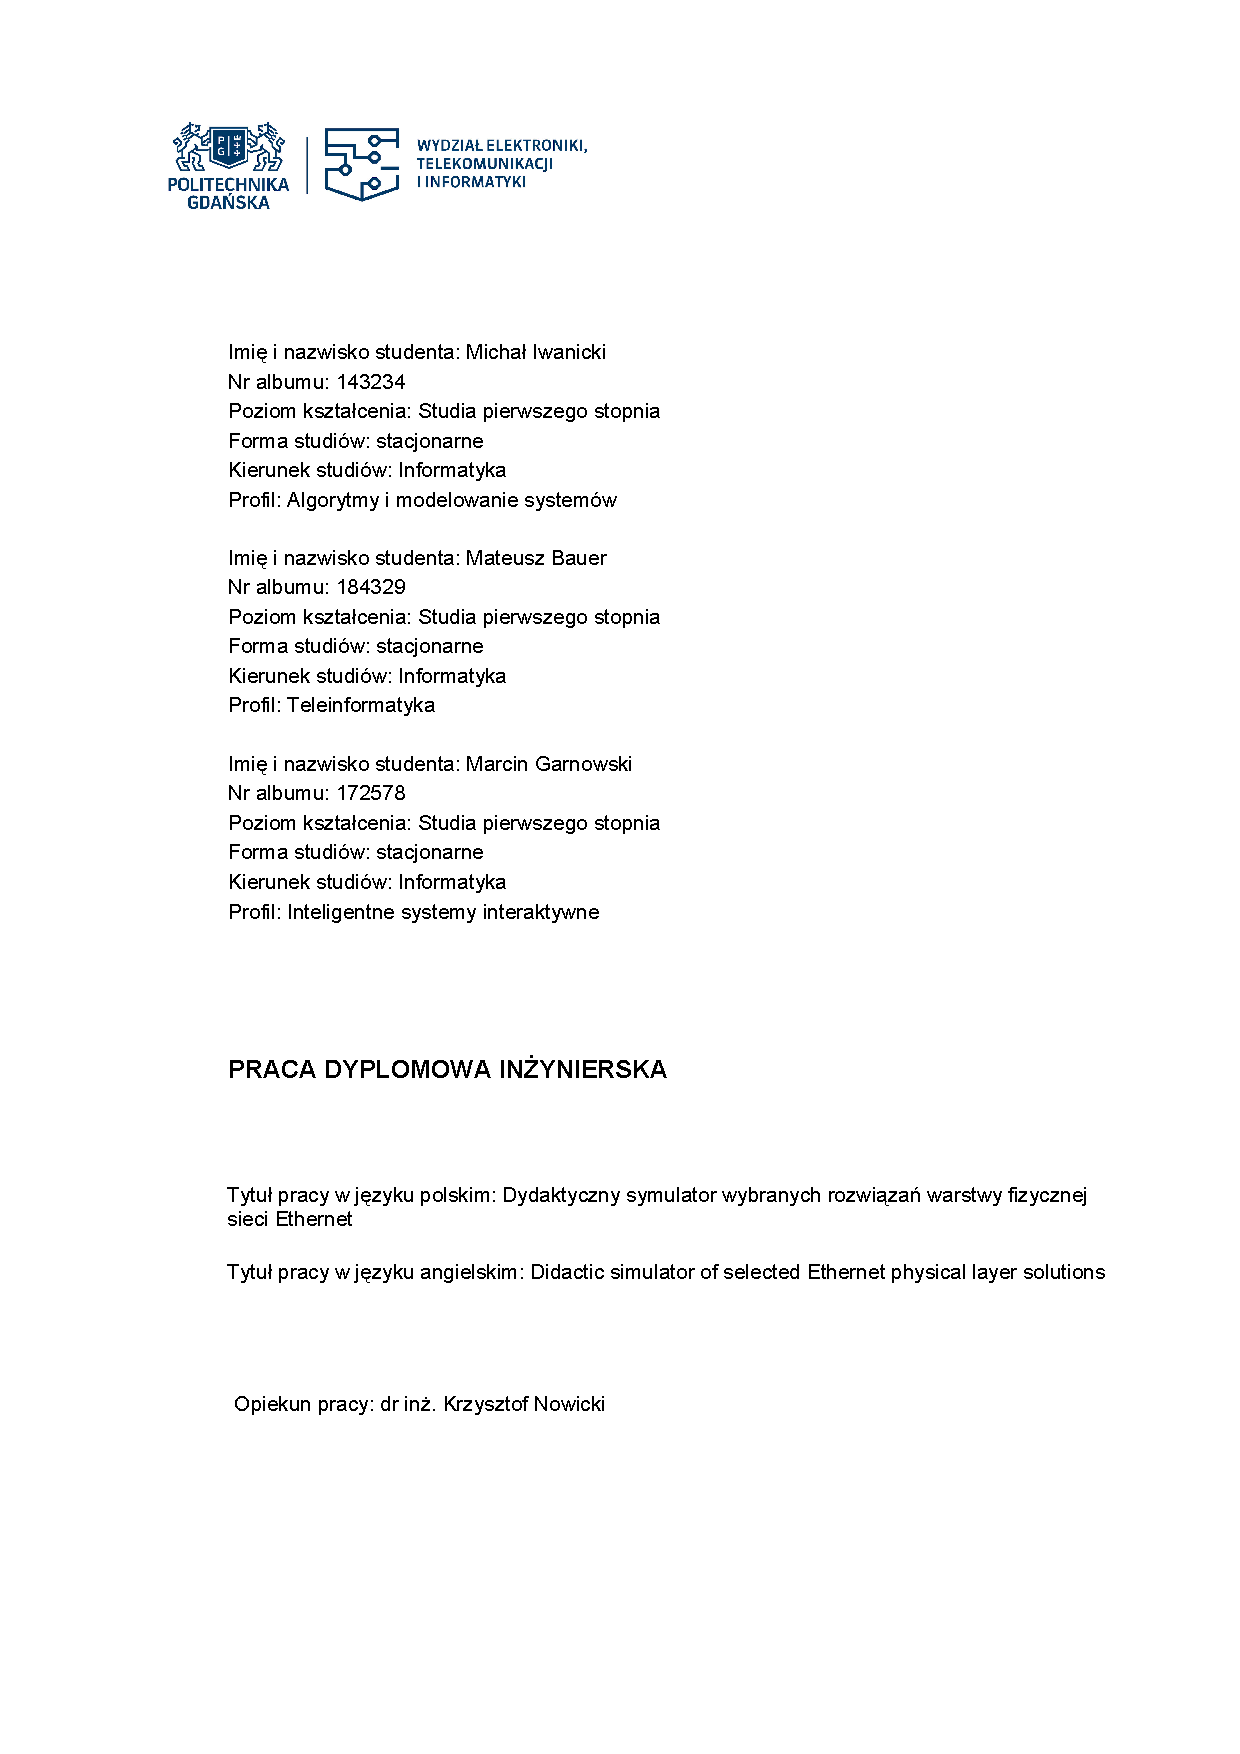
\includepdf[pages={1}]{StronaTytulowa.pdf}

\tableofcontents

\section*{Streszczenie}
\addcontentsline{toc}{section}{\protect\numberline{}Streszczenie}

Celem pracy jest stworzenie symulatora wybranych rozwiązań warstwy fizycznej sieci Ethernet oraz przeprowadzenie zajęc laboratoryjnych z grupą studentów. Wybrane rozwiązania to: kodowanie korekcyjne Reeda-Solomona oraz modulacja amplitudy impulsów (PAM). Dodatkowo zakres prac ograniczono do skrętki oraz konkretnego standardu - 40GBASE-T. Pierwszy rozdział wprowadza do kodowania korekcyjnego, przedstawiając wymaganą teorię matematyczną, jego właściwości oraz zastosowania w standardach Ethernet. Następnie przedstawiono potrzebę wykorzystania modulacji i różne jego rodzaje. Dla każdej modulacji wymienione są zalety i wady oraz wykorzystanie w standardach Ethernet. W kolejnym rozdziale obszernie opisany jest standard 40GBASE-T. Przybliża między innymi: możliwości tego standardu oraz techniki i rozwiązania, które są w nim wykorzystane, . Następna część dotyczy stworzonego symulatora. Zawiera przegląd dostępnych narzędzi oraz tych, które rzeczywiście wybrano, w tym: język programowania i biblioteki, Ostatnią częścią jest sprawozdanie z prowadzonego laboratorium. Opisuje zarówno przebieg samych zajęć dydaktycznych, jak i przygotowanie sali i sprzętu. Do pracy zostały załączone dodatki: instrukcja laboratoryjna, kod symulatora oraz instrukcja instalacji wraz z wymaganymi plikami na dołączonym urządzeniu przenośnym.

Słowa kluczowe: Ethernet, symulacja, laboratorium, skrętka, kodowanie korekcyjne Reeda-Solomona, PAM, Python.

\section*{Abstract}
\addcontentsline{toc}{section}{\protect\numberline{}Abstract}

The purpose of the work is to create a simulator of selected solutions of the physical layer of the Ethernet network and conduct laboratory classes with a group of students. The selected solutions are: Reed-Solomon error-correcting code and pulse-amplitude modulation (PAM). In addition, the scope of work was limited to twisted-pair and specific standard - 40GBASE-T. The first chapter introduces error-correcting coding, providing the required mathematical theory, its properties and applications in Ethernet standards. Afterwards, the need to use modulation and its different types are presented. For each modulation, the advantages, disadvantages and use in Ethernet standards are listed. The next chapter extensively describes the 40GBASE-T standard. It introduces, among other things: the capabilities of this standard and the techniques as well as solutions that are used in it. The next section deals with the simulator. It provides an overview of the available tools and those that were actually chosen, including: programming language and libraries, The last part is a report on the conducted laboratory classes. It describes both the course of the study itself and the preparation of the class room and equipment. The following appendices have been attached to the work: a laboratory instruction, simulator code and installation guide with the required files on the included data storage device.

Keywords: Ethernet, simulation, laboratory, twisted pair, Reed-Solomon error-correcting coding, PAM, Python.

\section{Środowisko programistyczne}
\subsection{Język programowania}

Do stworzenia symulatora wybrano język programowania Python z uwagi na kilka istotnych powodów. Przede wszystkim, czytelność składni stanowi ogromne ułatwienie podczas wspólnego tworzenia oprogramowania, a prostota pozwala skupić się na istocie problemu, nie tracąc czasu na pokonywanie trudności języka.

Dodatkowo, wybór Pythona jest motywowany chęcią rozwijania naszych umiejętności w tym środowisku, zarówno na poziomie indywidualnym, jak i zawodowym. Python cieszy się dużą popularnością jako uniwersalny język programowania, używany w różnych dziedzinach, takich jak analiza danych, sztuczna inteligencja czy aplikacje webowe. Posiadanie umiejętności programowania w Pythonie otwiera drzwi do szerszych możliwości zawodowych i dostępu do różnorodnych ciekawych projektów.

Jednym z najważniejszych argumentów przemawiających za wyborem Pythona jest jego ogromna popularność. Związana z tym społeczność programistyczna tworzy rozbudowany ekosystem, oferujący dostęp do wielu gotowych rozwiązań, bibliotek i frameworków. W kontekście tworzenia symulatora, istnieje wiele bibliotek w Pythonie, które mogą okazać się niezwykle przydatne. Na przykład, biblioteki umożliwiające tworzenie interfejsów graficznych ułatwią korzystanie z symulatora, biblioteki do analizy i przetwarzania sygnałów pomogą modelować różne aspekty transmisji, a biblioteki do wizualizacji pozwolą na przedstawienie wyników w przystępny sposób.

Inną cechą, która wyróżnia ten język programowania, jest jego przenośność. To ma dla nas duże znaczenie przy tworzeniu symulatora, który musi działać w warunkach laboratoryjnych, a więc na dowolnym popularniejszym systemie operacyjnym oraz charakteryzować się łatwością instalacji. Te wymagania Python w naszej ocenie spełnia.

\subsection{Narzędzia, biblioteki i moduły}
Jednym z celów postawionych przez promotora jest wykorzystanie gotowych rozwiązań podczas pracy nad symulatorem. W tym rozdziale zostaną przedstawione biblioteki i moduły języka Python oraz inne narzędzia, które mogą zostać wykorzystane w programie.

Python oferuje wiele bibliotek, które mogą okazać się kluczowe: od interfejsu graficznego po gotowe narzędzia do symulacji. Oto przegląd kilku z nich, na które brano pod uwagę przy projektowaniu rozwiązania:

\begin{enumerate}
    \item PyQt będzie biblioteką wykorzystywaną do stworzenia interfejsu graficznego użytkownika (GUI) dla symulatora. PyQt zapewnia szeroki zakres narzędzi do tworzenia rozbudowanych i przyjaznych użytkownikowi interfejsów, co jest szczególnie ważne w symulatorze dydaktycznym, gdzie interfejs musi być intuicyjny i nie stanowić niepotrzebnego wyzwania lub problemu dla biorących udział studentów
    \item NumPy jest najpopularniejszą biblioteką Python implementującą algorytmy matematyczne. Między innymi oferuje generatory liczb pseudolosowych o różnych rozkładach, co jest wymagane do prawidłowego generowania ramek ethernetowych i błędów
    \item  Matplotlib to popularna biblioteka do tworzenia wykresów. Może okazać się przydatna przy tworzeniu wykresów sygnałów
\end{enumerate}


Istnieją również inne popularne narzędzia, które mogą być użyteczne do symulacji rozwiązań warstwy fizycznej sieci Ethernet:
\begin{enumerate}
    \item SPICE (Simulation Program with Integrated Circuit Emphasis) jest powszechnie stosowanym narzędziem do symulacji obwodów elektronicznych. Jest to rozbudowany program, który umożliwia modelowanie i analizę zachowania obwodów złożonych, takich jak układy analogowe, cyfrowe czy mikroelektroniczne. W celu korzystania z tego narzędzia w środowisku Python dostępna jest biblioteka PySpice, będąca interfejsem umożliwiającym korzystanie ze SPICE,
    \item MATLAB to znane i powszechnie używane narzędzie do obliczeń numerycznych, analizy danych i modelowania systemów. Posiada szeroki zakres narzędzi i funkcji przeznaczonych do tworzenia modeli matematycznych, symulacji dynamicznych itp.,
    \item Scapy umożliwia tworzenie i przetwarzanie różnego rodzaju pakietów sieciowych, w tym ramek Ethernet, co jest kluczową funkcjonalnością symulatora.
\end{enumerate}

\section{Symulator}
\subsection{Interfejs użytkownika}
Interfejs użytkownika został wykonany przy użyciu PyQt5 oraz Qt Designer. Qt Designer to graficzne narzędzie do projektowania interfejsów użytkownika w ramach frameworka Qt. Umożliwia łatwe tworzenie i dostosowywanie wyglądu aplikacji oraz następne jego wygenerowanie jako kodu w języku Python lub C++.

Interfejs składa się z kilku zakładek stworzonych, które umożliwiają przełączanie między częściami aplikacji bez utraty wyników dotychczasowej pracy. Każda zakładka przeznaczona jest do innego zadania laboratoryjnego i zawiera symulacje innych rozwiązań ethernetowych. 

\begin{figure}[ht]
    \centering
    
\includegraphics{images/zakladki.png}
    \caption{Zakładki symulatora}
    \label{fig:zakladki_image}
\end{figure}

Wykresy są tworzone przy pomocy biblioteki Matplotlib. Została dodatkowo stworzona klasa, która zawiera stworzone wykresy i może być użyta jako element graficznego interfejsu użytkownika, a więc dodana do niego.

\subsection{Symulacje wybranych rozwiązań}
Aplikacja umożliwa symulowanie wybranych rozwiązań fizycznej warstwy sieci Ethernet. W każdym przypadku użytkownik ma swobodę podawania własnych parametrów wejściowych, zmieniania ich, co ma na celu ułatwienie zrozumienia działania tych rozwiązań.

\subsubsection{Kodowanie korekcyjne Reeda-Solomona}
Kodowanie korekcyjne Reed-Solomona to metoda kodowania korekcyjnego, mająca na celu wykrywanie i naprawianie błędów w przesyłanych danych. Stworzona została w 1960 roku przez dwóch amerykańskich matematyków: Irving S. Reed i Gustave Solomon. Od tego czasu znalazła szerokie zastosowanie w dziedzinie komunikacji, kodowaniu i obsłudze dysków.

Główną ideą kodowania korekcyjnego Reed-Solomona jest dodawanie nadmiarowych danych do przesyłanych informacji, dzięki czemu w przypadku wystąpienia błędów, możliwe jest ich wykrycie i skorygowanie. Algorytm opiera się na algebraicznych właściwościach ciał skończonych, co umożliwia efektywne wykonywanie operacji matematycznych potrzebnych do kodowania i dekodowania.

W symulatorze kodowanie i dekodowanie wykorzytuje metody klasy ReedSolomon udostępnionej w bibliotece galois. Jest ona rozszerzeniem, dodającym operacje na ciałach skończonych, innej popularnej biblioteki języka Python - NumPy. Jej nazwa pochodzi od nazwiska francuskiego matematyka Évariste Galois, który zasłynął badaniami ciał skończonych, które nazywane są również ciałami Galois.

\begin{figure}[ht]
    \centering
    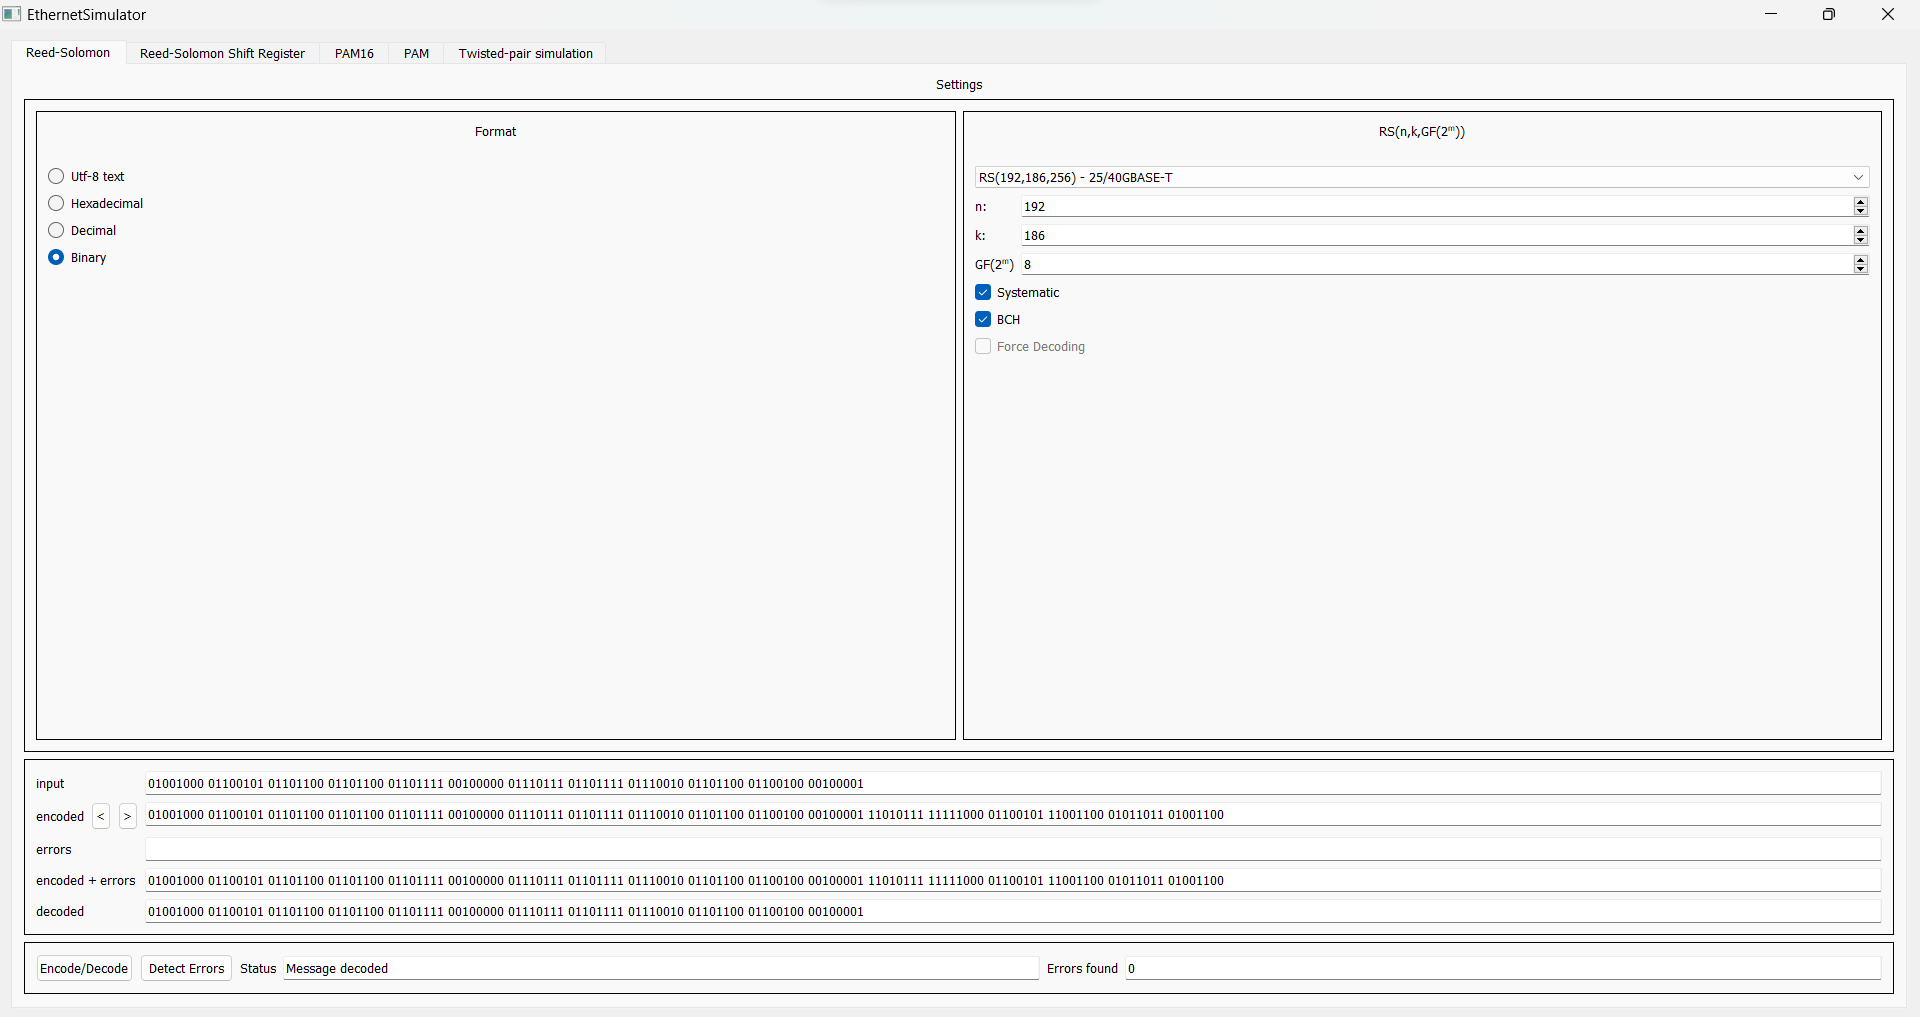
\includegraphics[width=\textwidth]{images/rs.png}
    \caption{Zakładka z kodowaniem Reeda-Solomona}
    \label{fig:rs_image}
\end{figure}

\subsubsection{Symulacja przesyłu sygnału}
Symulator umożliwia symulację przesyłu danych przez pojedynczą lub 4-parową skrętkę, w której można śledzić zmiany napięć. W tym przypadku wykorzystana została biblioteka PySpice. Dzięki niej można nadać wykorzystywanemu przewodowi pożądane parametry, między innymi: opór, długość i indukcyjność.

Użytkownik ma możliwość podawania tych parametrów w przewijalnym oknie, gdzie może dodawać również kolejne przewodniki. Patrz Table~\ref{tab:parametry}.

\begin{table}[ht]
    \centering
    \begin{tabular}{|c|c|c|c|}
        \hline
        \textbf{Parametr} & \textbf{Od} & \textbf{Do} & \textbf{Domyślnie} \\
        \hline
        Voltage offset & 0 & 10 & 0 \\
        Output impedance & 0 & 200 & 100 \\
        Length & 1 & 100 & 2 \\
        Resistence & 0 & 100 & 0.19 \\
        Inductance & 0 & 1000 & 525 \\
        Capacitance & 0 & 100 & 52 \\
        \hline
    \end{tabular}
    \caption{Parametry symulacji}
    \label{tab:parametry}
\end{table}

Symulacja wykonywana jest w osobnym wątku. Dodatkowo możliwa jest jednoczesna symulacja wielu przewodów o różnych parametrach, które następnie przedstawiane są na jednym wykresie. Opcjonalnie można ukrywać lub pokazywać wybrane symulacji zaznaczając odpowiednie pola przy listach parametrów odpowiednich przewodów.

\begin{figure}[ht]
    \centering
    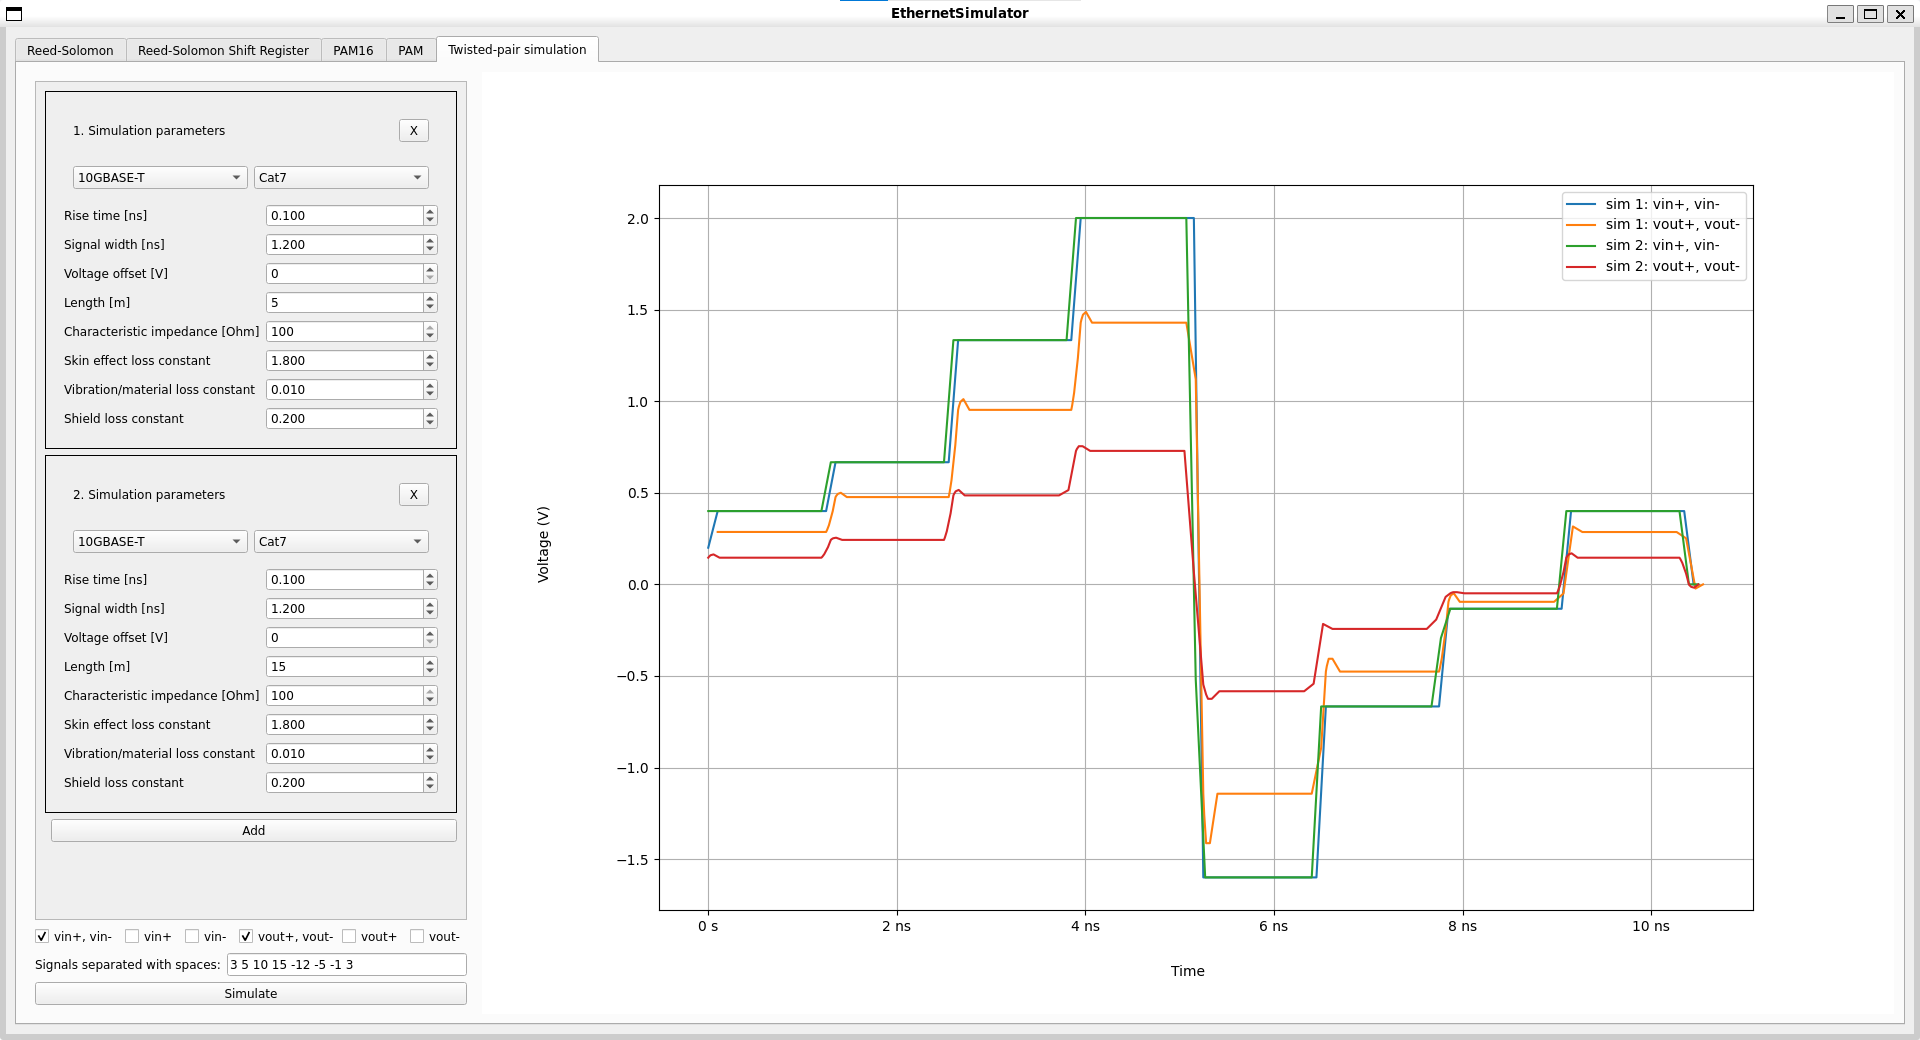
\includegraphics[width=\textwidth]{images/sim.png}
    \caption{Zakładka z symulacją}
    \label{fig:sim_png}
\end{figure}

\section{Kodowanie korekcyjne Reeda-Solomona}
\subsection{Wstęp}

Kodowanie korekcyjne Reeda-Solomona zostało stworzone przez Irvina S. Reeda
oraz Gustava Solomona w 1960 roku~\cite{Reed-Solomon-original}

Kody Reeda-Solomona charakteryzują się kilkoma parametrami~\cite{Reed-Solomon-Encoding-Decoding}:
\begin{itemize}
    \item alfabetem w ciele skończonym $\mathbb{F}_{p^m}$, $m>1$, $p$ jest liczbą
    pierwszą
    \item długością wiadomości $k$ do zakodowania $k < 2^{m}$
    \item długością słowa kodowego $n$ gdzie $k < n < 2^{m}$
    \item wielomianem generującym $g(x)$ dla kodów BCH
\end{itemize}

W kodach solomona wykorzystywanych w Ethernecie wykorzystujemy ciało $\mathbb{F}_2$ oraz ciała rozszerzone
$\mathbb{F}_{2^m}, m \in \{ 2, 3, \ldots \}$.

\subsection{Ciało skończone $\mathbb{F}_{q}$}

Aby zrozumieć działanie kodu Reeda-Solomona trzeba najpierw zrozumieć czym jest
ciało skończone $\mathbb{F}_q$ zwane też ciałem Galois $\operatorname{GF}(q)$.
Ciało to jest ciałem $K$ rzędu $q$ czyli takie które zawiera jedynie $q$ elementów.
Aby struktura algebraiczna była ciałem musi definiować 2 operacje zwane
dodawaniem i mnożeniem.
Te operacje muszą spełniać kilka warunków:

{\small
    \begin{align}
        a + (b + c) &= (a + b) + c & \forall a,b,c &\in K && \text{Łączność dodawania} \\
        a \cdot (b \cdot c) &= (a \cdot b) \cdot c & \forall a,b,c &\in K && \text{Łączność mnożenia} \\
        a + b &= b + a & \forall a,b &\in K && \text{Przemienność dodawania} \\
        a \cdot b &= b \cdot a & \forall a,b &\in K && \text{Przemienność mnożenia} \\
        a + 0 &= a & \forall a &\in K && \text{Element neutralny (0) dodawania} \\
        a \cdot 1 &= a & \forall a &\in K && \text{Element neutralny (1) mnożenia} \\
        a + (-a) &= 0 & \forall a &\in K && \text{Element odwrotny (-a) dodawania} \\
        a \cdot a^{-1} &= 1 & \forall a &\in K \setminus \{ 0 \} &&
            \text{Element odwrotny (} a^{-1} \text{) mnożenia} \label{field_mul_inverse}\\
        a \cdot (b + c) &= (a \cdot b) + (a \cdot c) & \forall a,b,c &\in K &&
            \text{Rozdzielność mnożenia względem dodawania}
    \end{align}
}%

Aby stworzyć ciało rzędu $p$ gdzie $p$ jest liczbą pierwszą można wykorzystać
pierścień klas reszt $\mathbb{Z} / p \mathbb{Z}$ z elementami~(\ref{modulo_elements})
i działaniem dodawania~(\ref{modulo_addition}) i mnożenia~(\ref{modulo_multiplication})

\begin{align}
    \modulo{p} = \{ [a]_p \; | \; a \in \mathbb{Z} \} &= \{ [0]_p, [1]_p,
    [2]_p, \ldots, [p-1]_p \} \label{modulo_elements} \\
    [a]_p + [b]_p &= [a + b]_p \label{modulo_addition} \\
    [a]_p \cdot [b]_p &= [a \cdot b]_p \label{modulo_multiplication}
\end{align}

Dla $p$ niebędących liczbami pierwszymi $\modulo{p}$ nie będzie
ciałem skończonym, ponieważ nie wszystkie elementy będą spełniały
warunek~(\ref{field_mul_inverse}).
Dla $\mathbb{F}_2$ działania $+$ i $*$ są równoważne operacjom logicznym XOR
oraz AND zdefiniowanymi w tablicy~\ref{truth_table:title}
\begin{table}[H]
    \captionof{table}{Dodawanie i mnożenie w $\mathbb{F}_2$}\label{truth_table:title}
    \centering
    \begin{tabular}{c c | c c}
        \toprule
        a & b & $+$ & $\cdot$ \\
        \midrule
        0 & 0 & 0 & 0 \\
        \midrule
        0 & 1 & 1 & 0 \\
        \midrule
        1 & 0 & 1 & 0 \\
        \midrule
        1 & 1 & 0 & 1 \\
        \bottomrule
    \end{tabular}
\end{table}

\subsection{Rozszerzone ciało skończone $\mathbb{F}_{2^m}$}

Aby stworzyć ciało skończone o rzędzie $2^m$, $k \in \{ 1, 2, 3, \ldots \}$ musimy
najpierw znaleźć nierozkładalny wielomian $p(x)$ stopnia $k$ o współczynnikach
$c_{n} \in \mathbb{F}_{2}$.
Elementami tego ciała będą wielomiany o postaci $c_{0} + c_{1}\alpha + c_{2}\alpha^{2} +
    \cdots + c_{k-1}\alpha^{k-1}$, $c_{n} \in \{0, 1\}$.
Zbiór tych elementów można zapisać jako zbiór wielomianów~(\ref{gf_extended:polynomial}),
zbiór k-krotek lub wartości binarnych zawierających współczynniki
wielomianu~(\ref{gf_extended:binary}).
\begin{align}
    \left\{ \sum_{n=0}^{k-1} c_{n}\alpha^{n} \,|\, c_{n} \in \{0,1\} \text{ for } 1 \le n \le k \right\}
        = \{ 0, 1, \alpha, 1 + \alpha, \alpha^{2}, \ldots, 1 + \alpha + \alpha^2 + \cdots + \alpha^{k-1} \}
        \label{gf_extended:polynomial} \\
    \{ 0, 1 \}^{k} = \{ (0, 0, 0, \ldots, 0), (1, 0, 0, \ldots, 0), (0, 1, 0, \ldots, 0),
    (1, 1, 0, \ldots, 0), \ldots, (1, 1, 1, \ldots, 1) \} \label{gf_extended:binary}
\end{align}

\subsection{Wykorzystanie w standardach Ethernetowych}

Różne kody Reeda-Solomona są wykorzystywane w wielu standardach Ethernet,
wyróżnione w tablicy~\ref{standards:title}

\begingroup
\hyphenpenalty10000
\exhyphenpenalty10000
\begin{table}[h]
\captionof{table}{Kodowania RS w różnych standardach~\cite{Ethernet}}\label{standards:title}
\centering
    \begin{tabular}{m{3cm} m{9cm}}
    \toprule
    Kodowanie RS    & Standardy \\
    \midrule
    RS(528,514)     & 10GBASE-R, 25GBASE-R, 100GBASE-CR4, 100GBASE-KR4, 100GBASE-SR4 \\
    \midrule
    RS(544,514)     & 50GBASE-R, 100GBASE-KP4, 100GBASE-CR2, 100GBASE-SR2, 100GBASE-DR, 100GBASE-FR1, 100GBASE-LR1, \hfill 200GBASE-R, \hfill 400GBASE-R \\
    \midrule
    RS(450,406)     & 1000BASE-T1 \\
    \midrule
    RS(192,186)     & 25GBASE-T, \;\;\;\;\;\;\;\;\;\;\;\;\; 40GBASE-T \\
    \midrule
    RS(360,326)     & 2.5GBASE-T1, \hfill 5GBASE-T1, \hfill 10GBASE-T1 \\
    \bottomrule
    \end{tabular}
\end{table}
\endgroup

\subsection{Właściwości kodu}
Kody Reeda-Solomona cechują się możliwością korekty $\lfloor \frac{n-k}{2} \rfloor$
oraz wykrycia $n-k$ błędnych symboli. Symbol w ciele $\mathbb{F}_{2^m}$ składa się
z $m$ bitów co w przypadku błędów grupowych daje możliwość korekty maksymalnie
$m \cdot \lfloor \frac{n-k}{2} \rfloor$ bitów bądź detekcji $m(n-k)$ przekłamanych
bitów

\subsection{Tworzenie kodu}
Istnieje wiele różnych sposobów tworzenia kodu które tworzą kod o innych właściwościach.


\subsubsection{Oryginalny sposób}
Sposób kodowania przedstawiony w pracy Reeda i Solomona polega na stworzeniu wielomianu $p_m(x)=\sum_{i=0}^{k-1}m_{i}x^i$, gdzie $m_i\in\mathbb{F}_q$ to $i$\nobreakdash-ty element wiadomości, po czym za pomocą tego wielomianu obliczane jest słowo kodowe $C(m)=(p_m(a_0), p_m(a_1), \ldots, p_m(a_{n-1}))$ gdzie $a_i$ to różne elementy ciała $\mathbb{F}_q$.

\subsubsection{Kod systematyczny}
\label{subsection:Kod systematyczny}
Za pomocą niewielkiej modyfikacji można stworzyć kod systematyczny czyli taki w którym słowo kodowe zawiera w sobie kodowaną wiadomość.
Żeby stworzyć kod systematyczny musimy zmodyfikować sposób tworzenia wielomianu w taki sposób by $p_m(x_i)=m_i$ dla $i \in \{0,1,\ldots,k-1\}$.

Jednym ze sposobów stworzenia takiego wielomianu jest użycie metody interpolacji wielomianów. Słowo kodowe wygenerowane z tego wielomianu będzie zawierało wiadomość w pierwszych $k$ elementach.
\[C(m)=(p_m(a_0), p_m(a_1), \ldots, p_m(a_{n-1})) = (m_0, m_1, \ldots, m_{k-1}, p_m(a_k), p_m(a_{k+1}), \ldots, p_m(a_{n-1}))\]

\subsubsection{Kod BCH}

Kody BCH~(Bose-Chaudhuri-Hocquenghem) są podklasą kodów cyklicznych co oznacza że każde przesunięcie słowa kodowego jest także słowem kodowym
\begin{align*}
    (c_0, c_1,\ldots, c_{n-2}, c_{n-1}), \;
    (c_{n-1}, c_0, \ldots, c_{n-3}, c_{n-2}),\ldots, \;
    (c_1, c_2, \ldots, c_{n-1}, c_{0})
\end{align*}

Aby zbudować kod BCH Reeda-Solomona potrzebujemy najpierw funkcji minimalnej pierwiastka $\alpha$, czyli takiego minimalnego wielomianu nierozkładalnego $p(x)$ stopnia $m$ dla którego istnieje element prymitywny $\alpha$ który pozwala wygenerować całe ciało skończone
\begin{align*}
    \mathbb{F}_{2^m} = \{0, 1, \alpha, \alpha^2, \ldots, \alpha^{p^{m}-1} \}
\end{align*}

Mając taki element prymitywny jesteśmy w stanie stworzyć wielomian generujący $g(x)$ używając wzoru
\begin{align*}
    t &= n - k \\
    g(x) = \prod_{i=0}^{t-1} (x - \alpha^i) &= g_{t}x^t + g_{t-1}x^{t-1} +
    \cdots + g_{1}x + g_{0}
\end{align*}
Aby utworzyć słowo kodowe $c(x)$ należy pomnożyć wielomian wiadomości $p_m(x)$ przez wielomian generujący $g(x)$: $c(x) = p_{m}(x) \cdot g(x)$

\subsubsection{Systematyczny kod BCH}

Aby uzyskać systematyczne słowo kodowe $c(x)$ musimy obliczyć:
\begin{align*}
    c_r(x) &= p_m(x) \cdot x^t \mod g(x) \\
    c(x) &= p_m(x) \cdot x^t - c_r(x)
\end{align*}

W standardzie Ethernet znajduje się przykładowa implementacja takiego kodu za pomocą rejestrów przesuwnych, przestawiona w pracy na rysunku~\ref{model-funkcjonalny}, $2t=n-k$
\begin{figure}[H]
    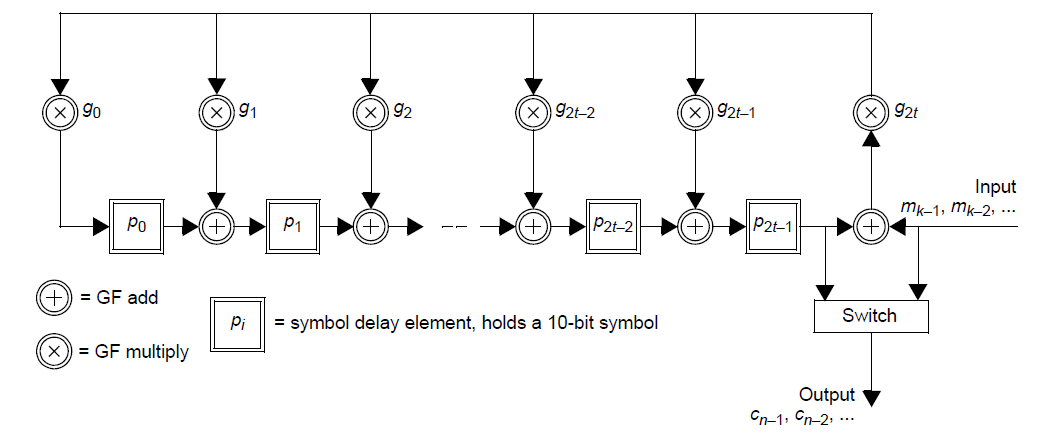
\includegraphics[width=0.95\textwidth,height=0.5\textheight,keepaspectratio]{rs-shift-register.png}
    \caption{Model funkcjonalny kodera RS~\cite[sekcja 91.5.2.7]{Ethernet}}\label{model-funkcjonalny}
\end{figure}


\section{Modulacja}

\subsection{Dlaczego potrzebujemy modulacji?}

Modulacja cyfrowa to technika zamiany bitów na sygnał oraz sygnału na bity. Jest kluczowym zagadnieniem w przesyle danych pomiędzy systemami komputerowymi. W odróżnieniu od modulacji analogowej, gdzie przesyłane dane wybierane są z przedziału,
modulacja cyfrowa operuje na dyskretnym zbiorze danych (bitach).

Dane reprezentowane są w postaci zmiany parametrów przesyłanego sygnału. Wyróżniane są cztery podstawowe metody:

\begin{enumerate}
    \item PSK (phase-shift keying) --- zmiana fazy fali nośnej sygnału,
    \item FSK (frequency-shift keying) --- zmiana częstotliwości fali nośnej sygnału,
    \item ASK (amplitude-shift keying) --- zmiana amplitudy fali nośnej sygnału,
    \item QAM (quadrature amplitude modulation) --- połączenie PSK oraz FSK, a więc zmieniana jest zarówno amplituda oraz faza.
\end{enumerate}

Zmiany sygnału (symbole) kodujące kolejne bity wybierane są ze skończonego zbioru nazywanego alfabetem modulacji.
Dział ten przedstawi popularne techniki modulacji w technologiach Ethernetowych.

\subsection{Wprowadzenie}

Aby ławiej zrozumieć ideę stojącą za bardziej skomplikowanymi technikami modulacji, należałoby na wprowadzeniu wyjaśnić kilka podstawowych pojęć.

Główną charakterystyką łącza jest szerokość pasma (ang. bandwidth) --- określa ona maksymalną (teoretyczną) liczbę bitów jaką łączę jest w stanie przesłać w danym czasie. Podawana jest ona w bitach na sekundę [$bps$] lub w hercach [Hz].

Przepustowość (ang. channel capacity) --- rzeczywista szerokość pasma, zmierzona w określonych warunkach.

Przepływność (ang. bit rate) --- rzeczywista ilość bitów transmitowanych w jednostce czasu poprzez kanał, podawana również w $bps$ lub Hz. Jest stałą charakterystyką danego łącza.

W 1924 roku Harry Nyquist przedstawił światu równanie, za pomocą którego określić można maksymalną przepływność łącza o szerokości pasma $B$ z wykorzystaniem $V$ poziomów:

\begin{align*}
    \text{Przepływność}_{max} &= 2B * log_{2}{V}
\end{align*}

24 lata później Claude Shannon rozszerzył równanie Nyquista, uwzględniając szum. Udowodnił on, że maksymalną przepływność łącza o szerokości pasma $B$ oraz stosunku sygnału do szumu $S/N$ można
obliczyć ze wzoru:

\begin{align*}
    \text{Przepływność}_{max} &= B * log_{2}{(1 + S/N)}
\end{align*}

Granica ta nazywana jest limitem Shannona.

Innym ważnym pojęciem jest multipleksacja (ang. multiplexing) i oznacza przesył wielu symboli jednocześnie w jednym kanale --- realizowany w postaci kilku przewodów, na które dane podawane są jednocześnie w każdym cyklu zegara.

\subsection{Non-Return-to-Zero}

Na początku rozważmy przykład. Najprostszą metodą byłoby używanie dodatniego napięcia dla bitu równego 1 i ujemnego napięcia dla 0.
Technika ta nosi nazwę \textbf{NRZ (Non-Return-to-Zero)}.
W praktyce wykorzystywana jest w połączeniu z kodowaniem liniowym np. 64b/66b, ale nie stosuje się tej techniki samoistnie.
Jest tak, ponieważ podczas przesyłania danych mogą wystąpić długie ciągi zer lub jedynek, a więc nadawany sygnał nie będzie się zmieniał.
Jest to zjawisko niepożądane podczas transmisji i może doprowadzić do desynchronizacji zegarów strony nadawczej i odbiorczej.

Rozważmy też przypadek, w którym nadawane jest naprzemiennie 1 i 0 --- otrzymamy wówczas okres równy 2 bity, co oznacza, że potrzebujemy pasma B/2 Hz przy prędkości B bit/s.
Nie trudno zauważyć, że do szybszego nadawnia zwiększona musi zostać szerokość pasma, co nie jest optymalnym rozwiązaniem z uwagi na ograniczoność tego zasobu \cite{Computer-networks-Tanenbaum}.

Jednym z rozwiązań tego problemu jest wykorzystanie większej ilości poziomów napięcia. W powyższym przykładzie zastosowane zostały dwa poziomy, a co za tym idzie mamy do dyspozycji dwa symbole przesyłane przez kanał.
Zwiększenie poziomów do 4 dałoby nam 4 różne symbole, a więc 2 bity informacji. W rezultacie przepływność wzrosła dwukrotnie, natomiast szerokość pasma nie zmieniła się. Technika zadziała pod warunkiem, że strona odbiorcza dysponuje sprzętem, który pozwoli jej na
rozróżnienie wielu poziomów napięcia. Jednakże w praktyce jest to koszt, który jesteśmy w stanie ponieść.

\subsection{Pulse-Amplitude Modulation}

Pulse-Amplitude Modulation (PAM) jest jedną z najpopularniejszych technik modulacji wykorzystywaną w technologiach Ethernetowych. Można ją również zobaczyć w innych technologiach (USB4, PCI Express 6.0). Jest to rodzaj modulacji, w którym dane przesyłane jako zmiany amplitudy sygnału. Modulacje PAM można podzielić na dwie kategorię:

\begin{enumerate}
    \item single polarity PAM --- do sygnału dodawana jest stała składowa, aby wartości napięcia były dodatnie
    \item double polarity PAM --- wartości mogą być ujemne lub dodatnie
\end{enumerate}

Modulacja PAM pozwala na przesył więcej niż jednego bitu w jednym takcie zegara, dzięki czemu zgodnie z równaniem Nyquista, zwiększona może zostać przepustowość przy niezmienionej szerokości pasma.
Poszczególne techniki PAM różnią się między sobą liczbą wykorzystywanych poziomów modulacji (technika NRZ może zatem być nazwana PAM2).
Liczba możliwych poziomów jest nieograniczona, jednak wraz ze wzrostem liczby poziomów, różnica pomiędzy symbolami maleje --- a to utrudnia stronie odbiorczej odczyt symboli. Dlatego właśnie rodzaj modulacji PAM wybiera się na podstawie możliwości strony nadawczej i odbiorczej. W systemach wbudowanych czy technologiach automotive wykorzystywanych jest mniej poziomów,
ponieważ w tych przypadkach liczy się kompaktowość, a przepływ danych nie jest duży. Zupełnie odwrotnie jest w technologiach Gigabit Ethernet, gdzie nie ma tak restrykcyjnych ograniczeń sprzętowych, a danych do przesyłu jest dużo.

Warto zwrócić uwagę na to, że wykorzystanie większej ilości poziomów nie adresuje problemu długich sekwencji samych zer lub jedynek. Dlatego również tu
stosuje się mechaznizmy zamiany wprowadzonych danych na bardziej zróżnicowany ciąg (np. kodowanie liniowe, skrambling).

\subsubsection{PAM3}

PAM3 --- trzypoziomowa modulacja PAM --- do przesyłu wykorzystuje wartości $+1$, $0$, $-1$. Jeden symbol koduje $log_{2}{3} \approx 1,58 \text{ bit/symbol}$.
PAM3 użyty został m.in. w standardach 100BASE-T4 (wczesna implementacja Fast Ethernet) i BroadR-Reach Ethernet standard --- wykorzystywany w branży automotive, opracowany przez firmę Broadcom Corporation.
Nie jest to schemat modulacji PAM, który często pojawia się w praktycznych rozwiązaniach z uwagi na to, że technologie wykorzystujące tę technikę nie zostały szeroko przyjęte.

Ciekawym aspektem jest podział bitów na symbole. Na pierwszy rzut oka widać, że istnieje problem z grupowaniem bitów --- nie można przecież przesłać $1,58$ bita. W modulacjach z liczbą poziomów będącą potęgą $2$ podział jest bardzo prosty --- bity grupujemy w dwójki, czwórki\dots i bezpośrednio mapujemy na symbole.

Tutaj rozwiązaniem jest tymczasowa zamiana bitów na trity (system trójkowy). Przykładowo w wersji drugiej USB4 dane dzieli się 11-bitowe grupy, po czym każda z nich zamienana jest na 7 tritów, osiągając przy tym
efektywność rzędu $\frac{11/7}{log_{2}{3}} * 100\% \approx 99\% $


\subsubsection{PAM4}

PAM4 --- czteropoziomowa modulacja PAM --- do przesyłu wykorzystuje wartości $3$, $1$, $-1$, $-3$, które kolejno odpowiadają logicznym wartościom 11, 10, 01, 00. W porównaniu do NRZ (Non-Return-to-Zero) ma przewagę posiadania dwukrotnie większej przepływność przy tej samej prędkości transmisji, co ilustruje poniższy rysunek \cite{Intel-pam4}:

\begin{figure}[ht]
    \centering
    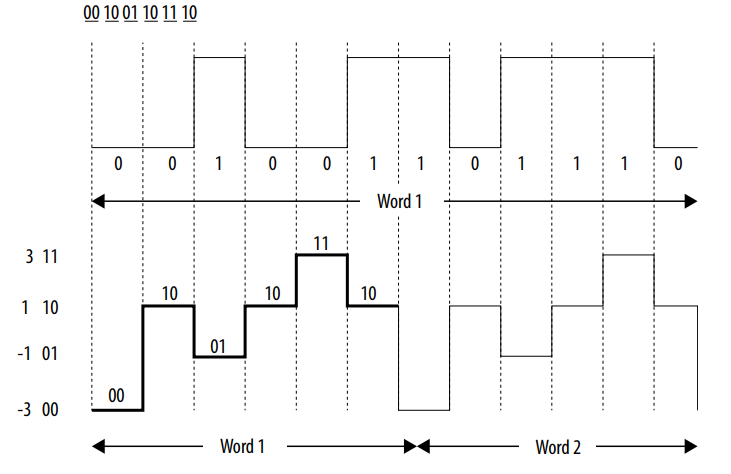
\includegraphics[width=\textwidth]{pam4_vs_nrz.png}
    \caption{Porównanie NRZ oraz PAM4}
    \label{fig:pam4_vs_nrz}
\end{figure}

Warto zwrócić uwagę na to, że w NRZ mamy jedno narastające zbocze ($0 \rightarrow 1$) i jedno opadające zbocze ($1 \rightarrow 0$), co daje dwie zmiany napięcia. W przypadku PAM4 jest to 6 narastających zbocz
($00 \rightarrow 01, 00 \rightarrow 10, 00 \rightarrow 11, 01 \rightarrow 10, 01 \rightarrow 11, 10 \rightarrow 11$) oraz 6 opadających zbocz
($11 \rightarrow 10, 11 \rightarrow 01, 11 \rightarrow 00, 10 \rightarrow 01, 10 \rightarrow 00, 01 \rightarrow 00$), które łącznie dają 12 różnych zmian napięcia.
Ma to znaczący wpływ na stosunek sygnału do szumu (SNR).

PAM4 stał się bardzo popularny w ostatnich latach i jest wykorzystywany m.in. w technologiach 100, 200 i 400 Gigabit Ethernet. Format ten został ustandaryzowany
także dla światłowodów (przykładowo 200GBASE-DR4).

\begin{figure}[ht]
    \centering
    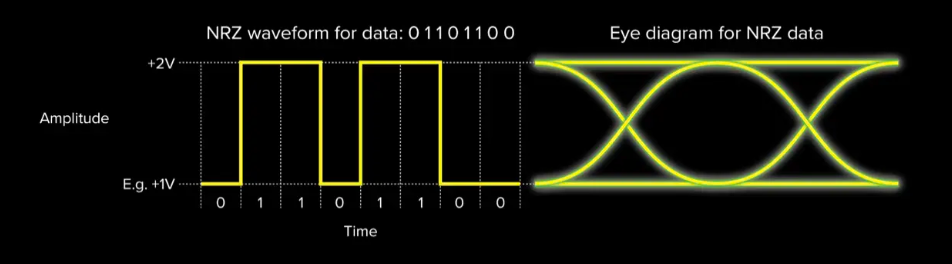
\includegraphics[width=\textwidth]{eye_diagram_nrz.png}
    \caption{Diagram oka NRZ}
    \label{fig:diagram_oka_nrz}
\end{figure}

\begin{figure}[ht]
    \centering
    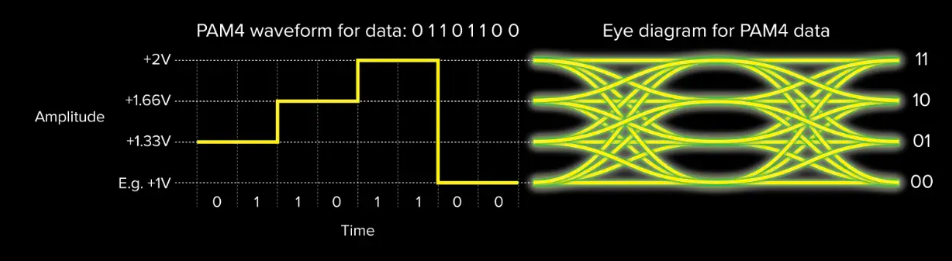
\includegraphics[width=\textwidth]{eye_diagram_pam4.png}
    \caption{Diagram oka PAM4}
    \label{fig:diagram_oka_pam4}
\end{figure}

\subsubsection{PAM16}

PAM16 --- szesnastopoziomowa modulacja PAM --- analogicznie do poprzednich przypadków wykorzystuje wartości $15$, $13$, $11$, \dots , $1$, $-1$, $-3$, \dots , $-13$, $-15$. Szesnaście poziomów daje 4 bity na symbol.
Modulacja PAM16 wykorzystywana jest w technologiach 10GBASE-T, 25GBASE-T czy 40GBASE-T.

\begin{figure}[ht]
    \centering
    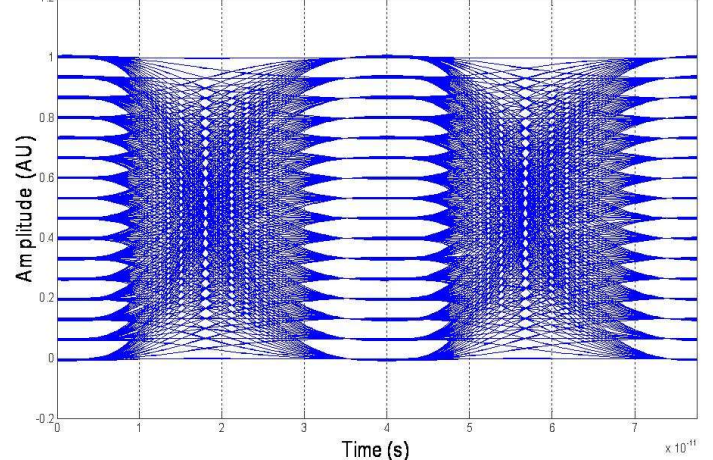
\includegraphics[width=\textwidth]{eye_diagram_pam16.png}
    \caption{Diagram oka PAM16}
    \label{fig:diagram_oka_pam16}
\end{figure}

\subsubsection{PAM --- podsumowanie}

Według artykułu \cite{Higher-order-modulation} przejście z PAM4 na modulacje wyższych rzędów podlega dyskusji. W przypadku PAM4, dwukrotnie większa liczba
poziomów niż w NRZ była opłacalna pomimo mniejszego stosunku sygnału do szumu (SNR). Jednakże przejście z PAM4 na PAM16 nie jest pod tym kątem wydajne, ponieważ
opiera się na bardziej wyrafinowanych technikach odczytu i interpretacji przesyłanych symboli, co wymaga większego zużycia energii.

Z drugiej strony modulacje PAM wyższych rzędów pozwalają na zwiększenie przepustowości w systemach z ograniczoną szerokością pasma --- co
umożliwia implementację technologii wielogigowych w skrętce --- dzięki czemu modulacja PAM16 przyjęła się w standardach 10GBASE-T, 25GBASE-T czy 40GBASE-T.

Te same technologie 10/25/40/50 GbE, które wykorzystują światłowód jako medium, a także technologie 200 GbE i 400 GbE używają NRZ oraz PAM4 z uwagi na prostotę.

\begingroup
\hyphenpenalty10000
\exhyphenpenalty10000
\begin{table}[h]
\captionof{table}{Modulacje w różnych standardach Ethernetowych}
\centering
    \begin{tabular}{m{3cm} m{3cm} m{3cm}}
    \toprule
    Standard & Medium & Modulacja \\
    \midrule
    1000BASE-T & skrętka & PAM5 \\
    \midrule
    1000BASE-T1 & skrętka & PAM3 \\
    \midrule
    1000BASE-KX & światłowód & NRZ \\
    \midrule
    10GBASE-T & skrętka & PAM16 \\
    \midrule
    10GBASE-SR & światłowód & NRZ \\
    \midrule
    25GBASE-T & skrętka & PAM16 \\
    \midrule
    25GBASE-SR & światłowód & NRZ \\
    \midrule
    40GBASE-T & skrętka & PAM16 \\
    \midrule
    50GBASE-SR & światłowód & PAM4 \\
    \midrule
    100GBASE-ZR & światłowód & PAM4 \\
    \midrule
    200GBASE-SR2 & światłowód & PAM4 \\
    \midrule
    400GBASE-SR4 & światłowód & PAM4 \\
    \bottomrule
    \end{tabular}
\end{table}
\endgroup


\section{40GBASE-T}

\subsection{Wprowadzenie}
40GBASE-T jest technologią transmitowania ramek Ethernetowych z prędkością 40 gigabitów na sekundę, wykorzystując skrętkę jako medium. Technologia została zdefiniowana po raz pierwszy jako część standardu IEEE 802.3ba w 2010 roku.

40GBASE-T zapewnia dwukierunkową komunikację przez cztery przewody skrętki. Każdy przewód transmituje ¼ zgromadzonych danych.

\subsection{Położenie 40GBASE-T w modelu OSI}

\begin{figure}[ht]
    \centering
    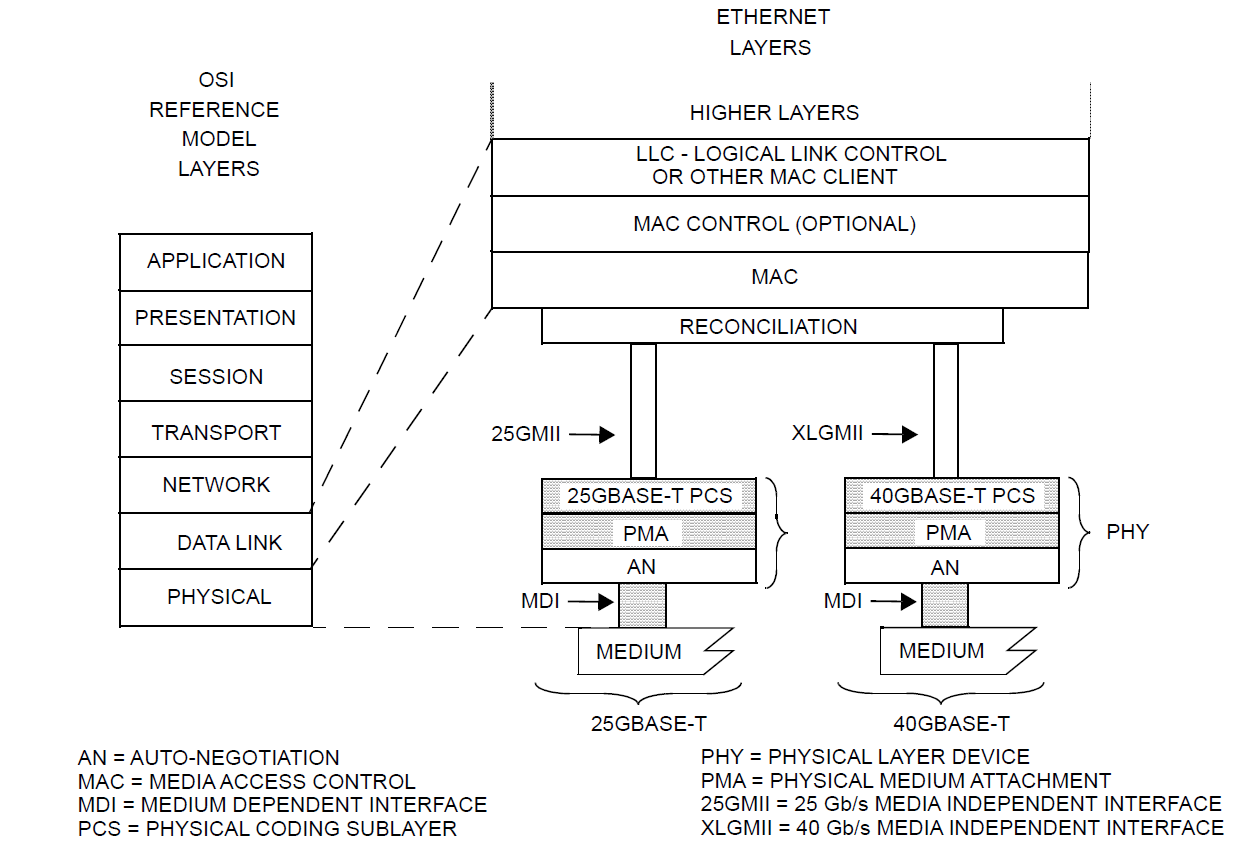
\includegraphics[width=\textwidth]{25-40-gbase-osi.png}
    \caption{Położenie 40GBASE-T w modelu OSI}
    \label{fig:40gbase-t_osi}
\end{figure}

\subsection{Media-Independent Interface}
MII czyli Media-Independent Interface to interfejs pomiędzy warstwą MAC oraz PHY. Powstał po to, aby warstwy MAC oraz PHY były niezależne od siebie - pozwala na pracę kontrolera MAC z warstwą PHY bez względu na to, jakie medium jest w użyciu.
W technologii 40GBASE-T MII określany jest jako XLGMII. Składa się z dwóch wektorów 64-bitowych TXD i RXD - odpowiedzialne za przesył danych w obu kierunkach, dwóch wektorów 8-bitowych TXC i RXC - wykorzystywane do przesyłu sygnałów kontrolnych oraz TX\_CLK i RX\_CLK - którymi podawany jest sygnał zegara. XLGMII pozwala na przesył danych na poziomie 40 Gb/s, w obu kierunkach.

\subsection{Warstwa PCS}\label{subsection:pcs}
40GBASE-T PCS (Physical Coding Sublayer) jest warstwą odpowiedzialną m.in. za kodowanie i dekodowanie oraz skramblowanie i deskramblowanie. W jej skład wchodzą m.in. skrambler i deskrambler, kodery i dekodery RS-FEC i LDPC oraz układ mapujący bity na DSQ128.
Dane trafiają z warstwy MAC do PCS przez XLGMII i gromadzone są w 64-bitowe bloki. Po zebraniu 50 takich bloków, pierwsze 48 z nich transkodowane są w 512-bitowe bloki, a pozostałe są do nich dołączane. Dane są następnie skramblowane i dołączany jest do nich bit pomocniczy (auxiliary bit), po czym dzielone są na dwa zbiory --- pierwszy z nich trafia do kodera Reed-Solomona, a drugi przetwarzany jest przez koder LDPC (Low density parity check). Otrzymuje się w ten sposób $512*3$ bitów zakodowanych przez RS-FEC oraz $512*4$ bitów --- LDPC, które łączone są w 7-bitowe grupy  ($u_0$, $u_1$, $u_2$), ($c_0$, $c_1$, $c_2$, $c_3$).

\subsection{Modulacja w 40GBASE-T}
Technologia 40GBASE-T wykorzystuje 16-poziomową modulację PAM - mając 16 różnych poziomów amplitudy możemy zakodować 16 różnych wartości co daje nam 4 bity danych.
Oprócz bitów niosących dane, przesyła się również bity pomocnicze (auxiliary bits), przez co w rzeczywistości jeden symbol PAM16 koduje 3,125 bitów informacji.
W ciągu każdej sekundy przesyłanych jest 3200 milionów symboli co przekłada się na prędkość transmisji równą 10 Gb/s (3,125 bit/symbol * 3200 MBd) na każdej z czterech par skrętki, co sumarycznie daje transmisję 40 Gb/s.

\subsubsection{Double Square Quadrature Amplitude Modulation}
Jak opisano w \ref{subsection:pcs}, warstwa PCS koduje otrzymane dane w 7-bitowe grupy. W technologii 40GBASE-T symbole nadawane przez warstwę PMA wybierane są z konstelacji DSQ128 (Double Square Quadrature Amplitude Modulation).

Aby wyjaśnić, czym jest DSQ128, pierw spójrzmy na modulację 64QAM. 64QAM (Quadrature Amplitude Modulation) to modulacja, która jest połączeniem modulacji amplitudy oraz fazy. Bity zamieniane są na symbole według diagramu konstelacji:

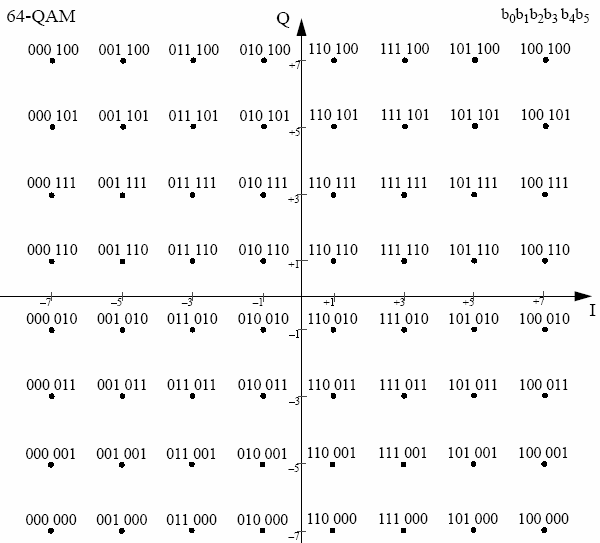
\includegraphics[scale=0.6]{64QAM-constellation-diagram.png}

Diagam podzielony jest na 4 sekcje, każda z nich zawiera 16 maksymalnie oddzielonych od siebie punktów. Punkty znajdujące się obok siebie różnią się jednym bitem --- dzięki czemu, gdy odbiorca otrzyma zły symbol, najprawdopodobniej tylko jeden bit będzie przekłamany.

DSQ128 jest złożeniem dwóch modulacji 64QAM i składa się z ośmiu sekcji, a każda z nich zawiera 16 punktów. Mając 7-bitową grupe ($u_0$, $u_1$, $u_2$), ($c_0$, $c_1$, $c_2$, $c_3$), pierwsze 3 bity definiują lewy dolny punkt w jednym z 8 regionów, natomiast na podstawie 4 kolejnych bitów wybierany jest jeden z 16 punktów w danym regionie. Proces ten opisany jest szczegółowo w \ref{mapowanie}

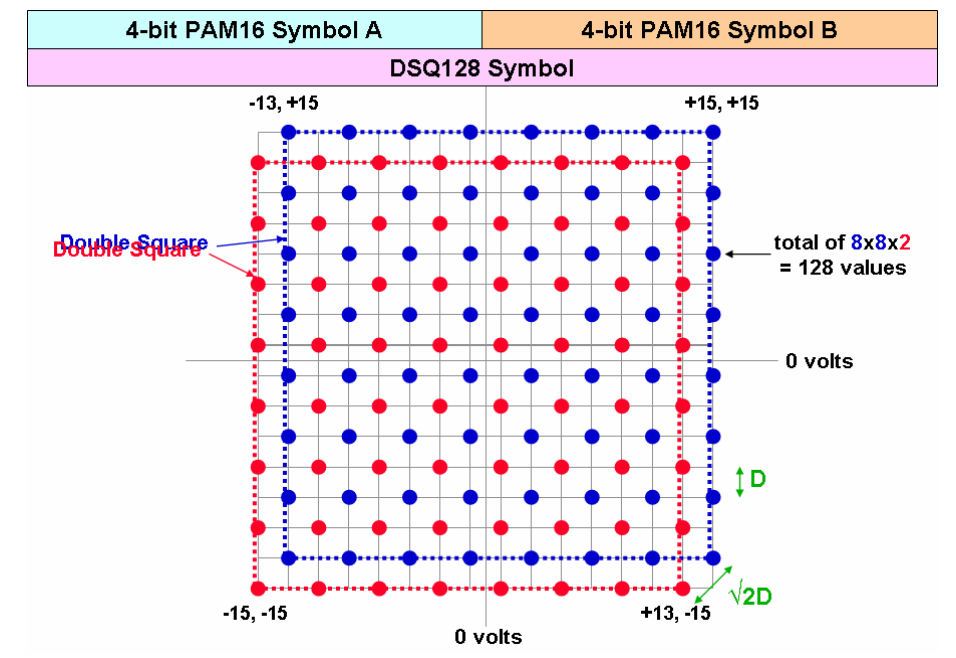
\includegraphics[scale=0.4]{dsq128.png}

\subsubsection{Mapowanie ramki LDPC na DSQ128}\label{mapowanie}
Zamianę 7-bitów ($u_0$, $u_1$, $u_2$), ($c_0$, $c_1$, $c_2$, $c_3$) pokazuje poniższy algorytm:

Krok 1:
\begin{align*}
    x_{13} &= \neg u_0 * u_2 \\
    x_{12} &= u_0 \oplus u_2 \\
    x_{11} &= c_0 \\
    x_{10} &= c_0 \oplus c_1 \\
    x_{23} &= (u_1 * u_2) + (u_0 * \neg u_1) \\
    x_{22} &= u_1 \oplus u_2 \\
    x_{21} &= c_2 \\
    x_{20} &= c_2 \oplus c_3
\end{align*}

Krok 2:
\begin{align*}
    x_1 &= 8x_{13} + 4x_{12} + 2x_{11} + x_{10} \\
    x_2 &= 8x_{23} + 4x_{22} + 2x_{21} + x_{20}
\end{align*}

Krok 3:
\begin{align*}
    y_1 &= (x_1 + x_2) \mod 16 \\
    y_2 &= (-x_1 + x_2) \mod 16
\end{align*}

Krok 4:
\begin{align*}
    \text{PAM16}_1 &= 2y_1 - 15 \\
    \text{PAM16}_2 &= 2y_2 - 15
\end{align*}

Otrzymane w ten sposób symbole są transmitowane na odpowiednich parach skrętki:

\begin{table}[h]
    \centering
    \resizebox{\textwidth}{!}{%
    \begin{tabular}{c | c c c c c c c |}
        \cmidrule{2-8}
        Pair A & PAM16$_1$<0> & PAM16$_2$<0> & PAM16$_1$<4> & PAM16$_2$<4> & \ldots & PAM16$_1$<508> & PAM16$_2$<508> \\
        \cmidrule{2-8}
        Pair B & PAM16$_1$<1> & PAM16$_2$<1> & PAM16$_1$<5> & PAM16$_2$<5> & \ldots & PAM16$_1$<509> & PAM16$_2$<509> \\
        \cmidrule{2-8}
        Pair C & PAM16$_1$<2> & PAM16$_2$<2> & PAM16$_1$<6> & PAM16$_2$<6> & \ldots & PAM16$_1$<510> & PAM16$_2$<510> \\
        \cmidrule{2-8}
        Pair D & PAM16$_1$<3> & PAM16$_2$<3> & PAM16$_1$<7> & PAM16$_2$<7> & \ldots & PAM16$_1$<511> & PAM16$_2$<511> \\
        \cmidrule{2-8}
    \end{tabular}}
\end{table}


\section{Symulator}
\subsection{Język programowania}

Do stworzenia symulatora wybrano język programowania Python z uwagi na kilka istotnych powodów. Przede wszystkim, czytelność składni stanowi ogromne ułatwienie podczas wspólnego tworzenia oprogramowania, a prostota pozwala skupić się na istocie problemu, nie tracąc czasu na pokonywanie trudności języka.

Dodatkowo wybór Pythona jest motywowany chęcią rozwijania naszych umiejętności w tym środowisku zarówno na poziomie indywidualnym, jak i zawodowym. Python cieszy się dużą popularnością jako uniwersalny język programowania, używany w różnych dziedzinach, takich jak analiza danych, sztuczna inteligencja czy aplikacje webowe. Posiadanie umiejętności programowania w Pythonie otwiera drzwi do szerszych możliwości zawodowych i dostępu do różnorodnych ciekawych projektów.

Jednym z najważniejszych argumentów przemawiających za wyborem Pythona jest jego ogromna popularność. Związana z tym społeczność programistyczna tworzy rozbudowany ekosystem, oferujący dostęp do wielu gotowych rozwiązań, bibliotek i frameworków. W kontekście tworzenia symulatora istnieje wiele bibliotek w Pythonie, które mogą okazać się niezwykle przydatne. Na przykład biblioteki umożliwiające tworzenie interfejsów graficznych ułatwią korzystanie z symulatora, biblioteki do analizy i przetwarzania sygnałów pomogą modelować różne aspekty transmisji, a biblioteki do wizualizacji pozwolą na przedstawienie wyników w przystępny sposób.

Inną cechą, która wyróżnia ten język programowania, jest jego przenośność. To ma dla nas duże znaczenie przy tworzeniu symulatora, który musi działać w warunkach laboratoryjnych, a więc na dowolnym popularniejszym systemie operacyjnym oraz charakteryzować się łatwością instalacji. Te wymagania Python w naszej ocenie spełnia.

\subsection{Narzędzia, biblioteki i moduły}
Jednym z celów postawionych przez promotora jest wykorzystanie gotowych rozwiązań podczas pracy nad symulatorem. W tym rozdziale zostaną przedstawione biblioteki i moduły języka Python oraz inne narzędzia, które mogą zostać wykorzystane w programie.

Python oferuje wiele bibliotek, które mogą okazać się kluczowe: od interfejsu graficznego po gotowe narzędzia do symulacji. Oto przegląd kilku z nich, które brano pod uwagę przy projektowaniu rozwiązania:

\begin{enumerate}
    \item PyQt będzie biblioteką wykorzystywaną do stworzenia interfejsu graficznego użytkownika (GUI) dla symulatora. PyQt zapewnia szeroki zakres narzędzi do tworzenia rozbudowanych i przyjaznych użytkownikowi interfejsów, co jest szczególnie ważne w symulatorze dydaktycznym, gdzie interfejs musi być intuicyjny i nie stanowić niepotrzebnego wyzwania lub problemu dla biorących udział studentów
    \item NumPy jest najpopularniejszą biblioteką Python implementującą algorytmy matematyczne. Między innymi oferuje generatory liczb pseudolosowych o różnych rozkładach, co jest wymagane do prawidłowego generowania ramek ethernetowych i błędów
    \item  Matplotlib to popularna biblioteka do tworzenia wykresów. Może okazać się przydatna przy tworzeniu wykresów sygnałów
\end{enumerate}


Istnieją również inne popularne narzędzia, które mogą być użyteczne do symulacji rozwiązań warstwy fizycznej sieci Ethernet:
\begin{enumerate}
    \item SPICE (Simulation Program with Integrated Circuit Emphasis) jest powszechnie stosowanym narzędziem do symulacji obwodów elektronicznych. Jest to rozbudowany program, który umożliwia modelowanie i analizę zachowania obwodów złożonych, takich jak układy analogowe, cyfrowe czy mikroelektroniczne. W celu korzystania z tego narzędzia w środowisku Python dostępna jest biblioteka PySpice, będąca interfejsem umożliwiającym korzystanie ze SPICE,
    \item MATLAB to znane i powszechnie używane narzędzie do obliczeń numerycznych, analizy danych i modelowania systemów. Posiada szeroki zakres narzędzi i funkcji przeznaczonych do tworzenia modeli matematycznych, symulacji dynamicznych itp.,
    \item Scapy umożliwia tworzenie i przetwarzanie różnego rodzaju pakietów sieciowych, w tym ramek Ethernet, co jest kluczową funkcjonalnością symulatora.
\end{enumerate}

\subsection{Interfejs użytkownika}\label{subsection:interfejs}
Interfejs użytkownika został wykonany przy użyciu PyQt5 oraz Qt Designer. Qt Designer to graficzne narzędzie do projektowania interfejsów użytkownika w ramach frameworka Qt. Umożliwia łatwe tworzenie i dostosowywanie wyglądu aplikacji oraz następne jego wygenerowanie jako kodu w języku Python lub C++.

Interfejs składa się z kilku zakładek (Rysunek~\ref{fig:zakladki_sim_image}), które umożliwiają przełączanie między częściami aplikacji bez utraty wyników dotychczasowej pracy. Każda zakładka przeznaczona jest do innego zadania laboratoryjnego i zawiera symulacje innych rozwiązań ethernetowych. 

\begin{figure}[H]
    \centering
    
\includegraphics{images/zakladki.png}
    \caption{Zakładki symulatora}
    \label{fig:zakladki_sim_image}
\end{figure}

Wykresy przedstawione na Rysunku~\ref{fig:sim_png} są tworzone przy pomocy biblioteki Matplotlib. Została dodatkowo stworzona klasa, która zawiera stworzone wykresy i może być użyta jako element graficznego interfejsu użytkownika, a więc dodana do niego.

\subsection{Symulacje wybranych rozwiązań}
Aplikacja umożliwa symulowanie wybranych rozwiązań fizycznej warstwy sieci Ethernet. W każdym przypadku użytkownik ma swobodę podawania własnych parametrów wejściowych, zmieniania ich, co ma na celu lepsze zrozumienie działania tych rozwiązań.

\subsubsection{Kodowanie korekcyjne Reeda-Solomona}
Kodowanie korekcyjne Reed-Solomona to metoda kodowania korekcyjnego, mająca na celu wykrywanie i naprawianie błędów w przesyłanych danych. Stworzona została w 1960 roku przez dwóch amerykańskich matematyków: Irving S. Reed i Gustave Solomon. Od tego czasu znalazła szerokie zastosowanie w dziedzinie komunikacji, kodowaniu i obsłudze dysków.

Główną ideą kodowania korekcyjnego Reed-Solomona jest dodawanie nadmiarowych danych do przesyłanych informacji, dzięki czemu w przypadku wystąpienia błędów, możliwe jest ich wykrycie i skorygowanie. Algorytm opiera się na algebraicznych właściwościach ciał skończonych, co umożliwia efektywne wykonywanie operacji matematycznych potrzebnych do kodowania i dekodowania.

W symulatorze kodowanie i dekodowanie wykorzytuje metody klasy ReedSolomon udostępnionej w bibliotece galois. Jest ona rozszerzeniem, dodającym operacje na ciałach skończonych, innej popularnej biblioteki języka Python - NumPy. Jej nazwa pochodzi od nazwiska francuskiego matematyka Évariste Galois, który zasłynął badaniami ciał skończonych, które nazywane są również ciałami Galois.

Zakładkę z kodowaniem Reeda-Solomona przedstawia Rysunek~\ref{fig:rs_png}.

\begin{figure}[H]
    \centering
    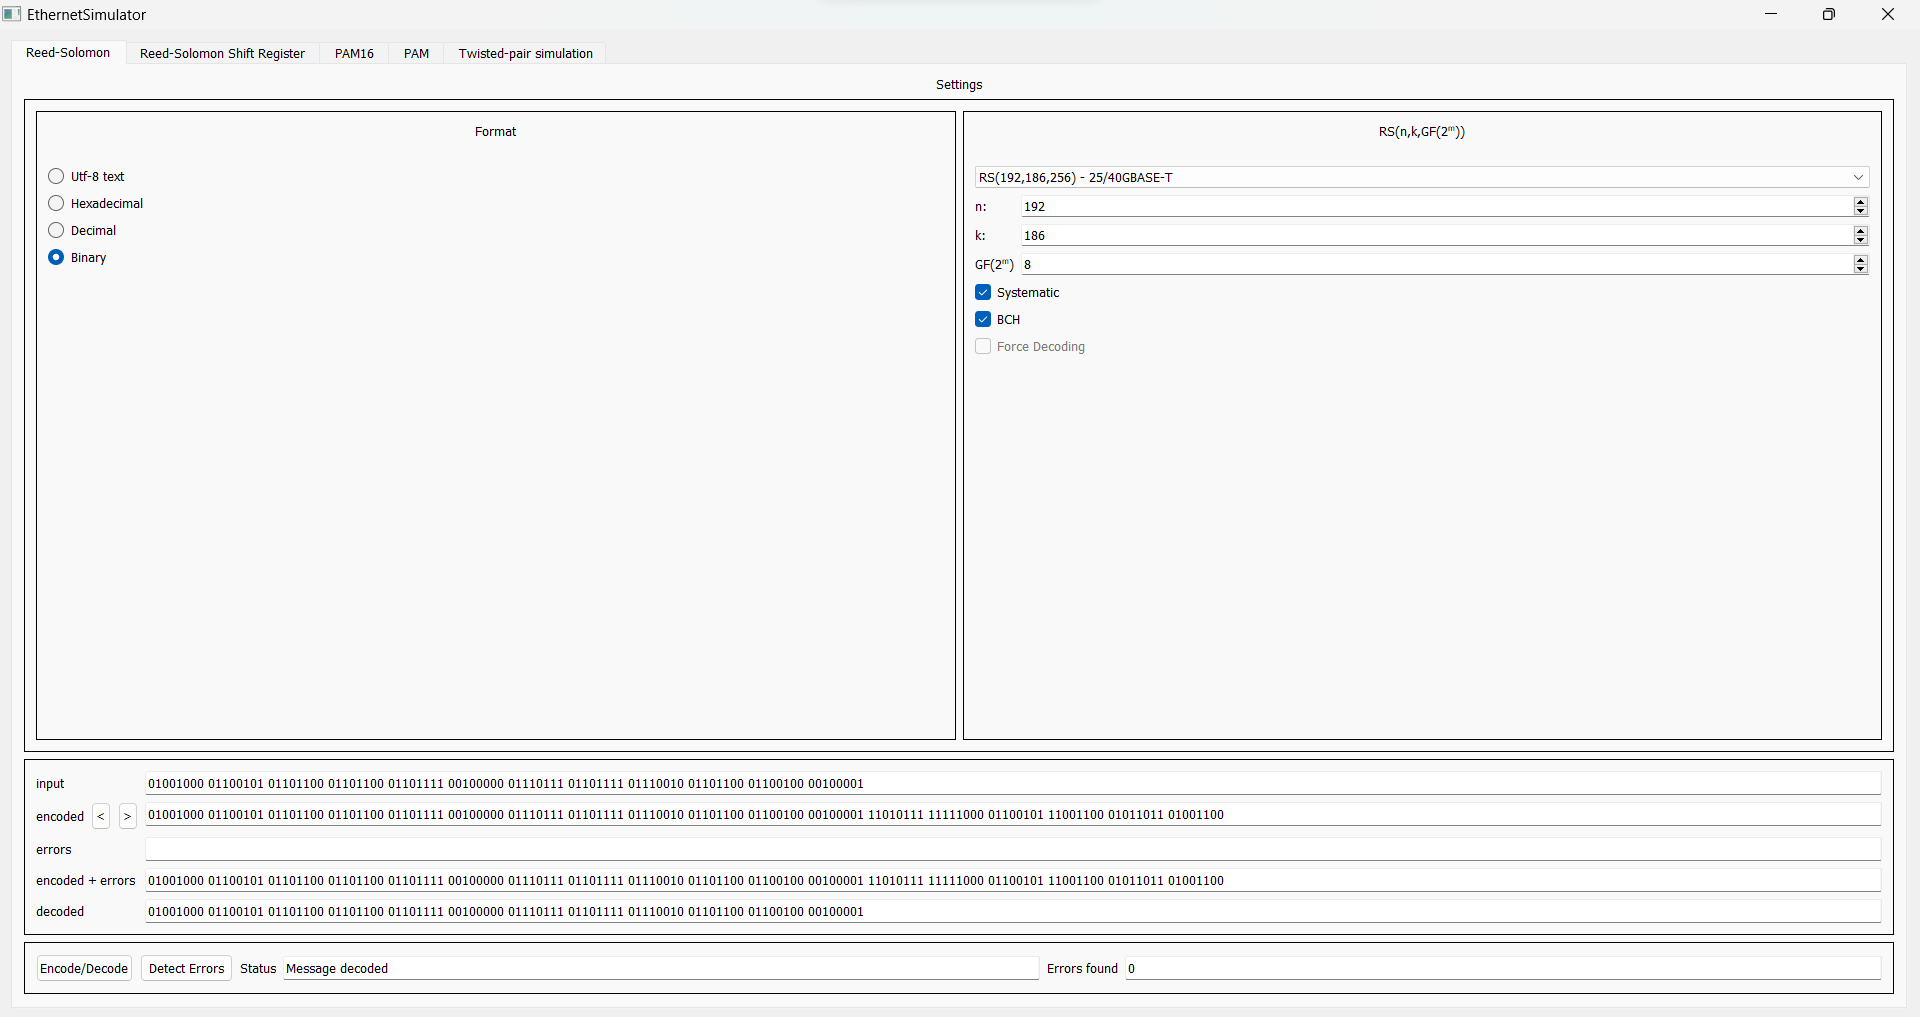
\includegraphics[width=\textwidth]{images/rs.png}
    \caption{Zakładka z kodowaniem Reeda-Solomona}
    \label{fig:rs_png}
\end{figure}

\subsubsection{Rejestr przesuwający dla kodowania Reeda-Solomona}

W tej zakładce (Rysunek~\ref{fig:rs_sr_png}) koder RS został zaimplementowany zgodnie z modelem
funkcyjnym udostępnionym w standarcie Ethernet. Po przejściu
wszystkich symboli wiadomości element `Switch' zaczyna przepuszczać symbole parzystości.
W opcjach po lewej stronie możemy podobnie jak w poprzedniej zakładce wybrać
parametry kodera oraz dodatkowo wybrać inne wielomiany i elementy prymitywne. Przycisk `Calculate generating polynomial' oblicza
wielomian generujący, a `Calculate primitive poly/ement' oblicza element i wielomian prymitywny dla podanego ciała skończonego $\mathbb{F}_{2^m}$.
Po prawej stronie mamy dane wejściowe oraz aktualny stan rejestrów $p_i$. `Fill symbol' jest symbolem, który będzie wysyłany, jeżeli zabraknie symboli na wejściu.

\begin{figure}[H]
    \centering
    \includegraphics[width=\textwidth]{images/rs-register-tab.png}
    \caption{Zakładka z rejestrem przesuwającym kodowania Reeda-Solomona}
    \label{fig:rs_sr_png}
\end{figure}

\subsubsection{PAM16}

Zakładka PAM16 (Rysunek ~\ref{fig:pam16_sim_png}) przedstawia przesył danych podanych w formacie szesnastkowym przez użytkownika przez czteroparową skrętkę.

\begin{figure}[H]
    \centering
    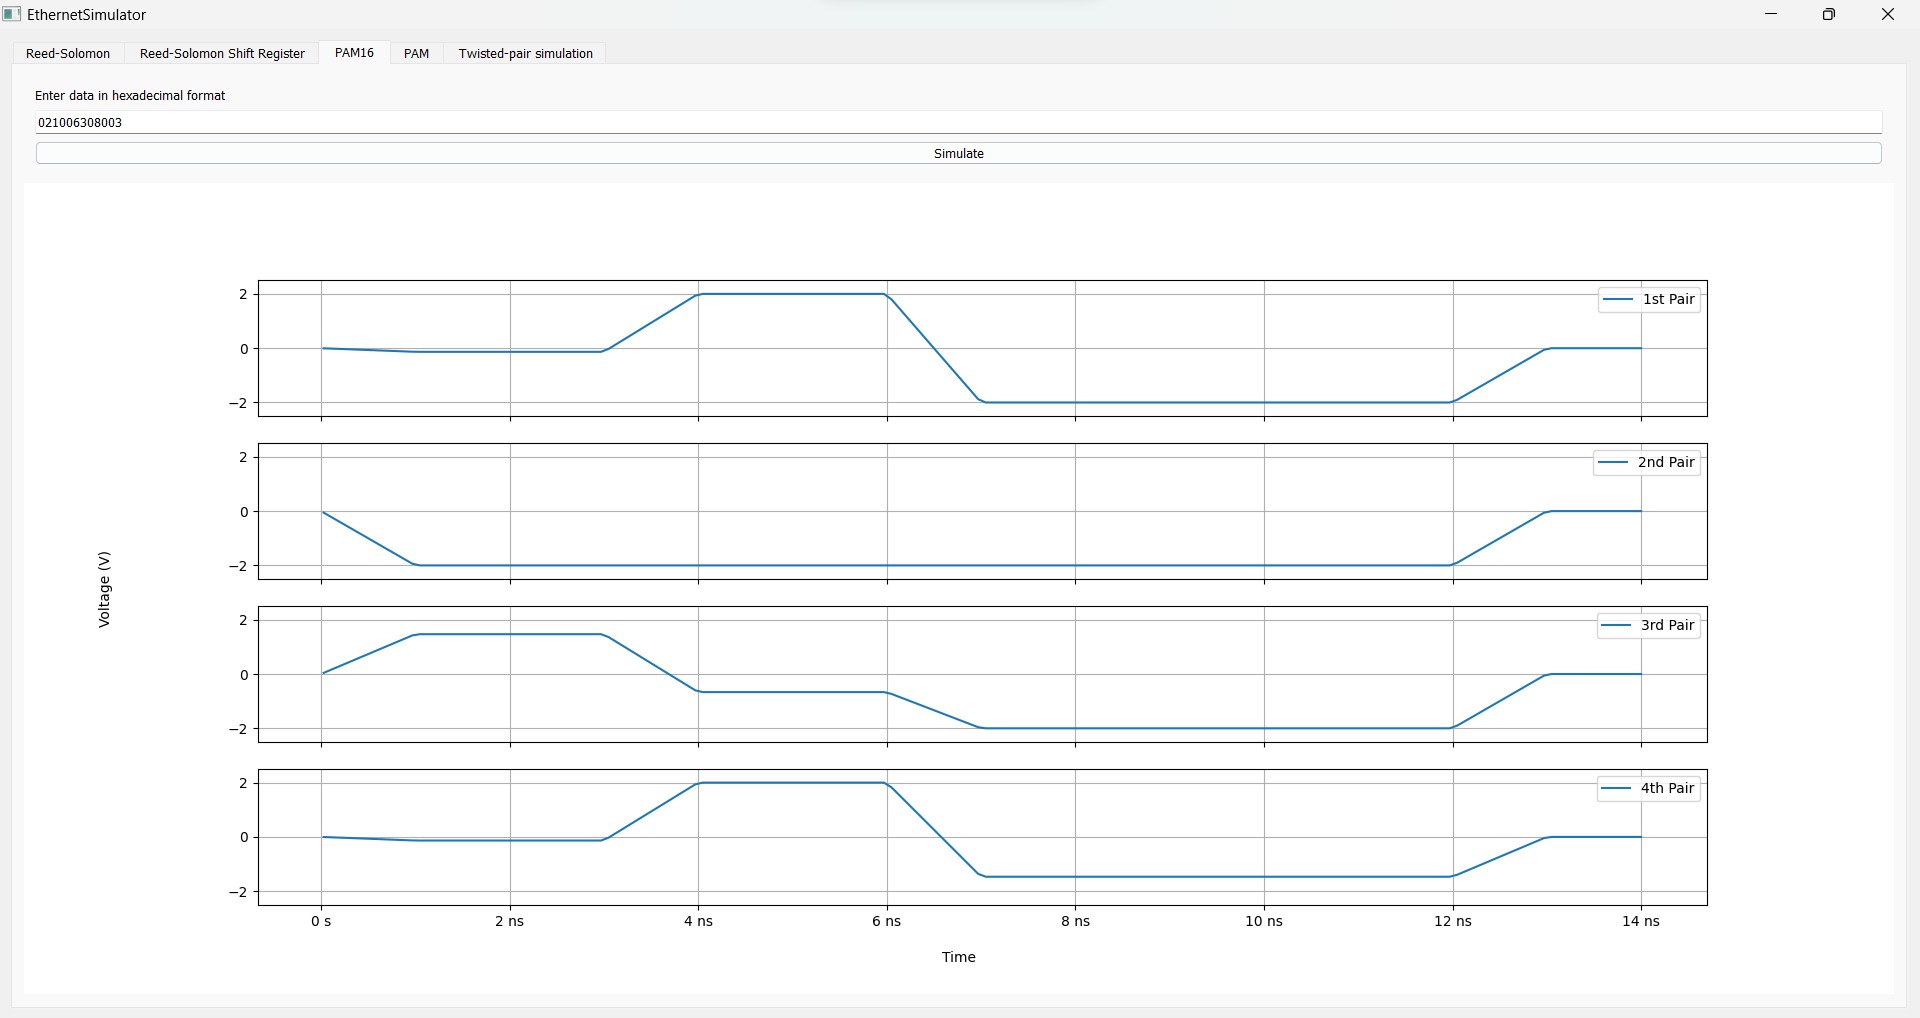
\includegraphics[width=\textwidth]{images/prezentacja_pam16.png}
    \caption{Zakładka z PAM16}
    \label{fig:pam16_sim_png}
\end{figure}

\subsubsection{PAM}

Zakładka PAM (Rysunek ~\ref{fig:pam_sim_png}) przedstawia różnice modulacji: NRZ, PAM4, PAM16. Symulacje są tworzone tak, jak w poprzedniej zakładce, na podstawie danych w formacie szesnastkowym podanych przez użytkownika.

\begin{figure}[H]
    \centering
    \includegraphics[width=\textwidth]{images/pam_tab.png}
    \caption{Zakładka z różnymi modulacjami}
    \label{fig:pam_sim_png}
\end{figure}

\subsubsection{Symulacja przesyłu sygnału}
Symulator (Rysunek ~\ref{fig:sim_png}) umożliwia symulację przesyłu danych przez pojedynczą cskrętkę, w której można śledzić zmiany napięć. W tym przypadku wykorzystana została biblioteka PySpice. Dzięki niej można nadać wykorzystywanemu przewodowi pożądane parametry, między innymi: opór, długość i indukcyjność.

\begin{figure}[H]
    \centering
    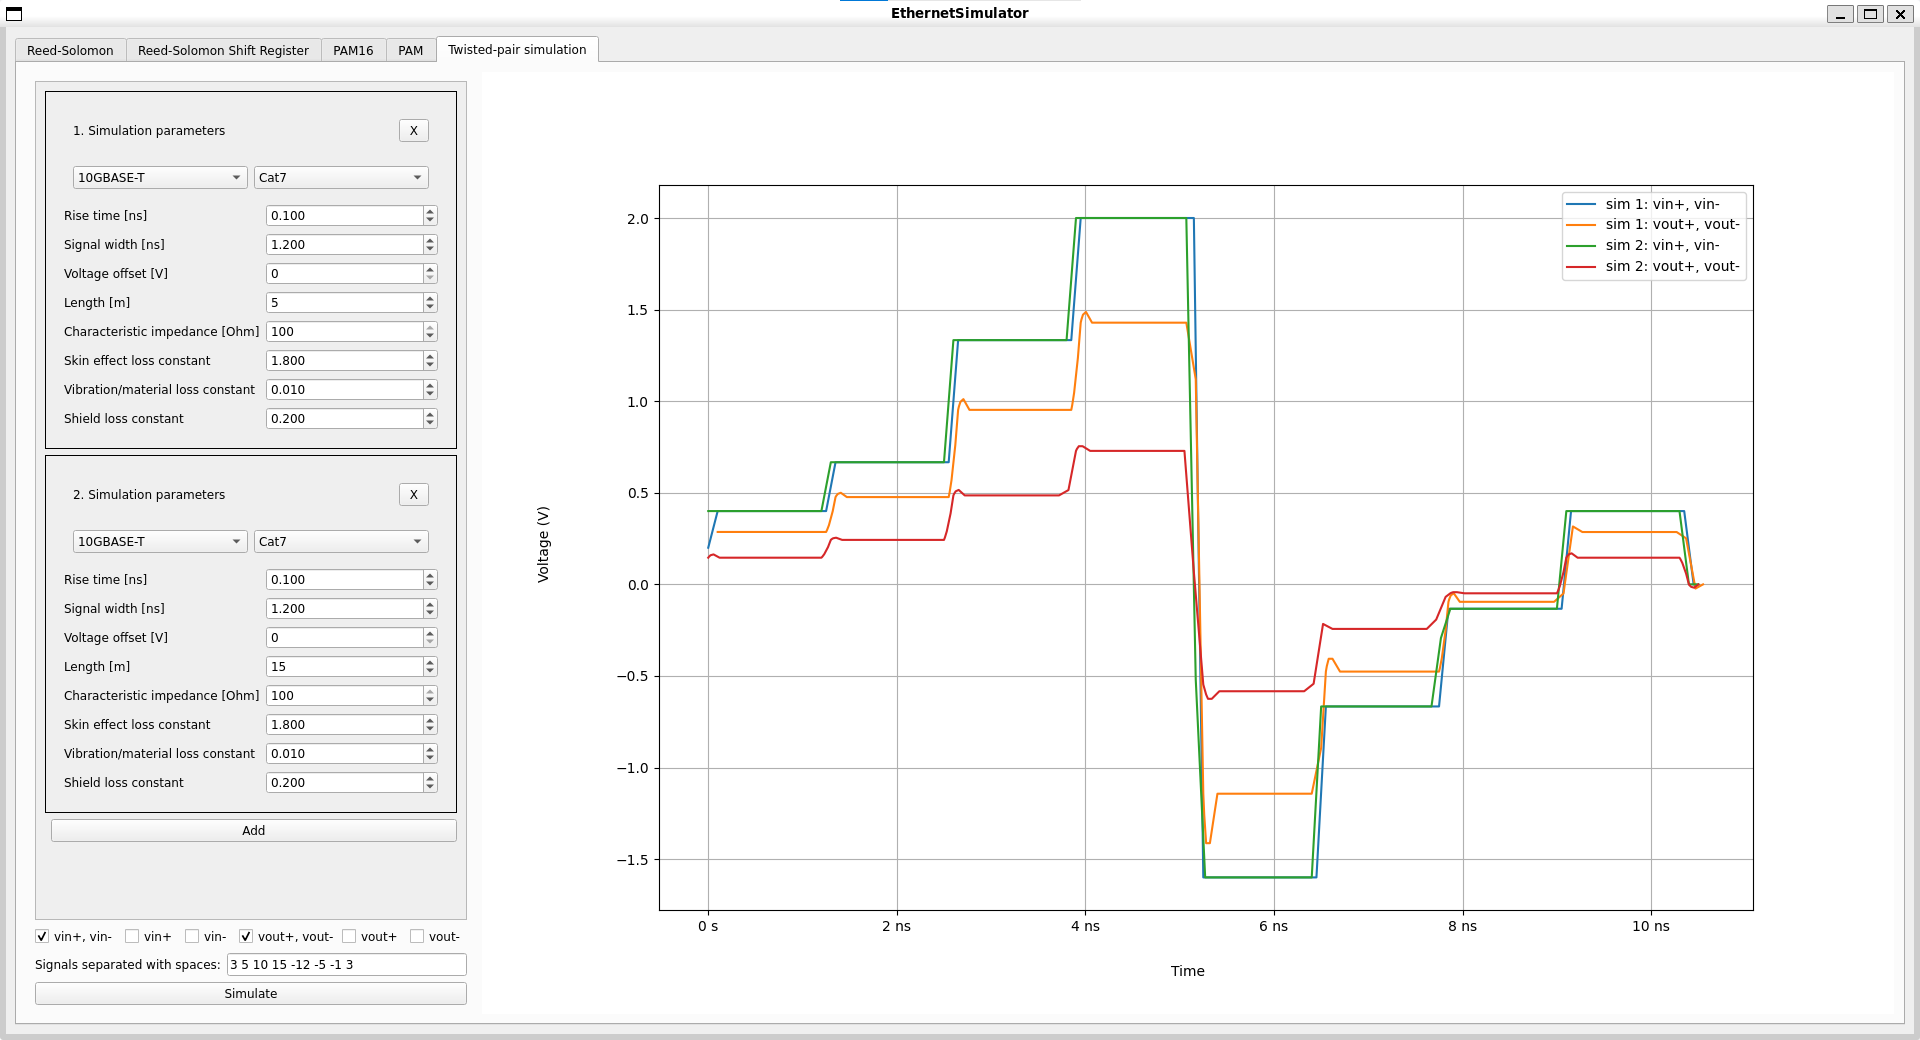
\includegraphics[width=\textwidth]{images/sim.png}
    \caption{Zakładka z symulacją}
    \label{fig:sim_png}
\end{figure}

Użytkownik ma możliwość podawania tych parametrów w przewijalnym oknie, gdzie może dodawać również kolejne przewodniki. Patrz Tabela~\ref{tab:parametry}.

\begin{table}[H]
    \captionof{table}{Parametry symulacji}
    \centering
    \begin{tabular}{|c|c|c|c|}
        \hline
        \textbf{Parametr} & \textbf{Od} & \textbf{Do} & \textbf{Domyślnie} \\
        \hline
        Voltage offset & 0 & 10 & 0 \\
        Output impedance & 0 & 200 & 100 \\
        Length & 1 & 100 & 2 \\
        Resistence & 0 & 100 & 0.19 \\
        Inductance & 0 & 1000 & 525 \\
        Capacitance & 0 & 100 & 52 \\
        \hline
    \end{tabular}
    \label{tab:parametry}
\end{table}

Symulacja wykonywana jest w osobnym wątku. Dodatkowo możliwa jest jednoczesna symulacja wielu przewodów o różnych parametrach, które następnie przedstawiane są na jednym wykresie. Opcjonalnie można ukrywać lub pokazywać wybrane symulacji zaznaczając odpowiednie pola przy listach parametrów odpowiednich przewodów.


\section{Zajęcia dydaktyczne --- sprawozdanie}
\subsection{Wprowadzenie}

Jak wspomniano wcześniej, zakres pracy inżynierskiej obejmuje przeprowadzenie zajęć laboratoryjnych opisanych w sekcji \ref{zajecia-dydaktyczne}.
Pierwsze zajęcia miały charakter testowy --- poza dydaktyką chciano: wychwycić potencjalne błędy w opracowanym symulatorze; sprawdzić czy studenci
potrafią zrealizować zadania laboratoryjne po przeczytaniu instrukcji; przygotować dyplomantów na problemy, które mogą pojawić się podczas prowadzenia
zajęć (awaria sprzętu, niekompatybilność oprogramowania na różnych systemach operacyjnych, niemożność zainstalowania oprogramowania ze względu na brakujące
biblioteki lub wersje bibiotek na komputerach). Problemy, które pojawiły się w trakcie pierwszych zajęć, zostały wychwycone przez autorów, ażeby
ostateczna wersja była możliwie najlepsza.

\subsection{Przygotowanie zajęć}
\subsubsection{Stan początkowy}
Przygotowania sali do zajęć dydaktycznych z grupą studentów rozpoczęły się pięć dni przed planowanymi zajęciami. Sala jest laboratorium dyplomowym dostępnym dla dyplomantów wydziału ETI Politechniki Gdańskiej. W momencie, gdy rozpoczęto przygotowania dostępnych było osiem komputerów stacjonarnych. Różniły się one zainstalowanymi systemami operacyjnymi: na połowie był to Windows 10, a na połowie Ubuntu 18.

\subsubsection{Podjęte działania}
W pierwszej kolejności spróbowano zainstalować i uruchomić symulator na komputerze z Ubuntu 18. Instalacja przez Internet okazała się niemożliwa ze względu na nieprzygotowanie zależności pod specyfikę tego systemu operacyjnego. Windows 10 okazał się bezproblemowy i, po użyciu dwóch poleceń: instalacja i uruchomienie symulatora, symulator był gotowy do używania.

W związku z problemami na Ubuntu 18 zdecydowano się zainstalować na tych komputerach Linux Mint. Po tym czasochłonnym procesie symulator uruchamiał się, jednak napotkano kolejny problem - okno symulatora było za duże ze wględu na wykorzystaną w programie ilustrację. Naprawiono to dodając do polecenia uruchomienia symulatora dwa opcjonalne parametry określające wielkość okna. 

W tym momencie sala była w ocenie prowadzących gotowa do przeprowadzenia zajęć. Ostatecznie dostępne były cztery komputery z Windows 10 oraz cztery komputery z Linux Mint.

\subsubsection{Problemy}
Podczas przygotowywania sali napotkano następujące problemy:
\begin{itemize}
    \item W sali istnieje problem z dostępem do Internetu na więcej niż jednym komputerze,
    \item Monitory dostępne w sali miały specyficzne proporcje,
    \item Dla Ubuntu 18 nie było w repozytorium potrzebnych zależności,
    \item Na Linux Mint okno programu rozszerzało się do wymiarów większych niż dostępna wielkosć monitora bez możliwości zmniejszenia,
    \item Aplikacja nie działała dla Pythona 3.12 ze względu na niedostępną w tej wersji bibliotekę libngspice.
\end{itemize}

\subsection{Przebieg zajęć}

Przed zajęciami wprowadzono ostatnie zmiany i poprawki do wejściówki oraz zadań laboratoryjnych. Wydrukowano je w nadmiarowej liczbie, by promotor, recenzent i prowadzący również mieli do nich dostęp.

Laboratoria odbyły się na wydziale ETI Politechniki Gdańskiej. Na początku zrealizowano wprowadzenie teoretyczne do omawianych zagadnień w postaci godzinnego
wykładu, który został przeprowadzony przez dyplomantów dla grupy studentów pod okiem promotora.

Następnie podzielono studentów na dwie grupy: pierwsza odbyła zajęcia tego samego dnia, druga --- tydzień później. Świadomą decyzją prowadzących uczestnicy zajęć nie byli uprzedzeni o systemach operacyjnych dostępnych na poszczególnych komputerach, więc zajmowali miejsca losowo. Zajęcia rozpoczęto od wejściówki (Dodatek B), a następnie zrealizowano zadania opracowane w ramach pracy (Dodatek C).

W trakcie zajęć studenci wykonywali zadania samodzielnie, konsultując się przy tym między sobą. Autorzy niniejszej pracy
byli do ich dyspozycji, po to aby rozwiać wszelkie nieścisłości, nakierować studentów na właściwe rozwiązanie i tym podobne.

Uczestnicy zajęć mieli okazję zaznajomić się z zagadnieniami, które występują w warstwie fizycznej Ethernet, natomiast
opracowany symulator pomógł w wizualizacji tychże rozwiązań --- porównanie zachowania sygnału w przypadku różnych metod modulacji oraz
sprawdzenie działania i właściwości kodera Reeda-Solomona. Rysunek~\ref{fig:zajecia_lab_zdjecie} przedstawia zdjęcie wykonane podczas pierwszych zajęć.

\begin{figure}[H]
    \centering
    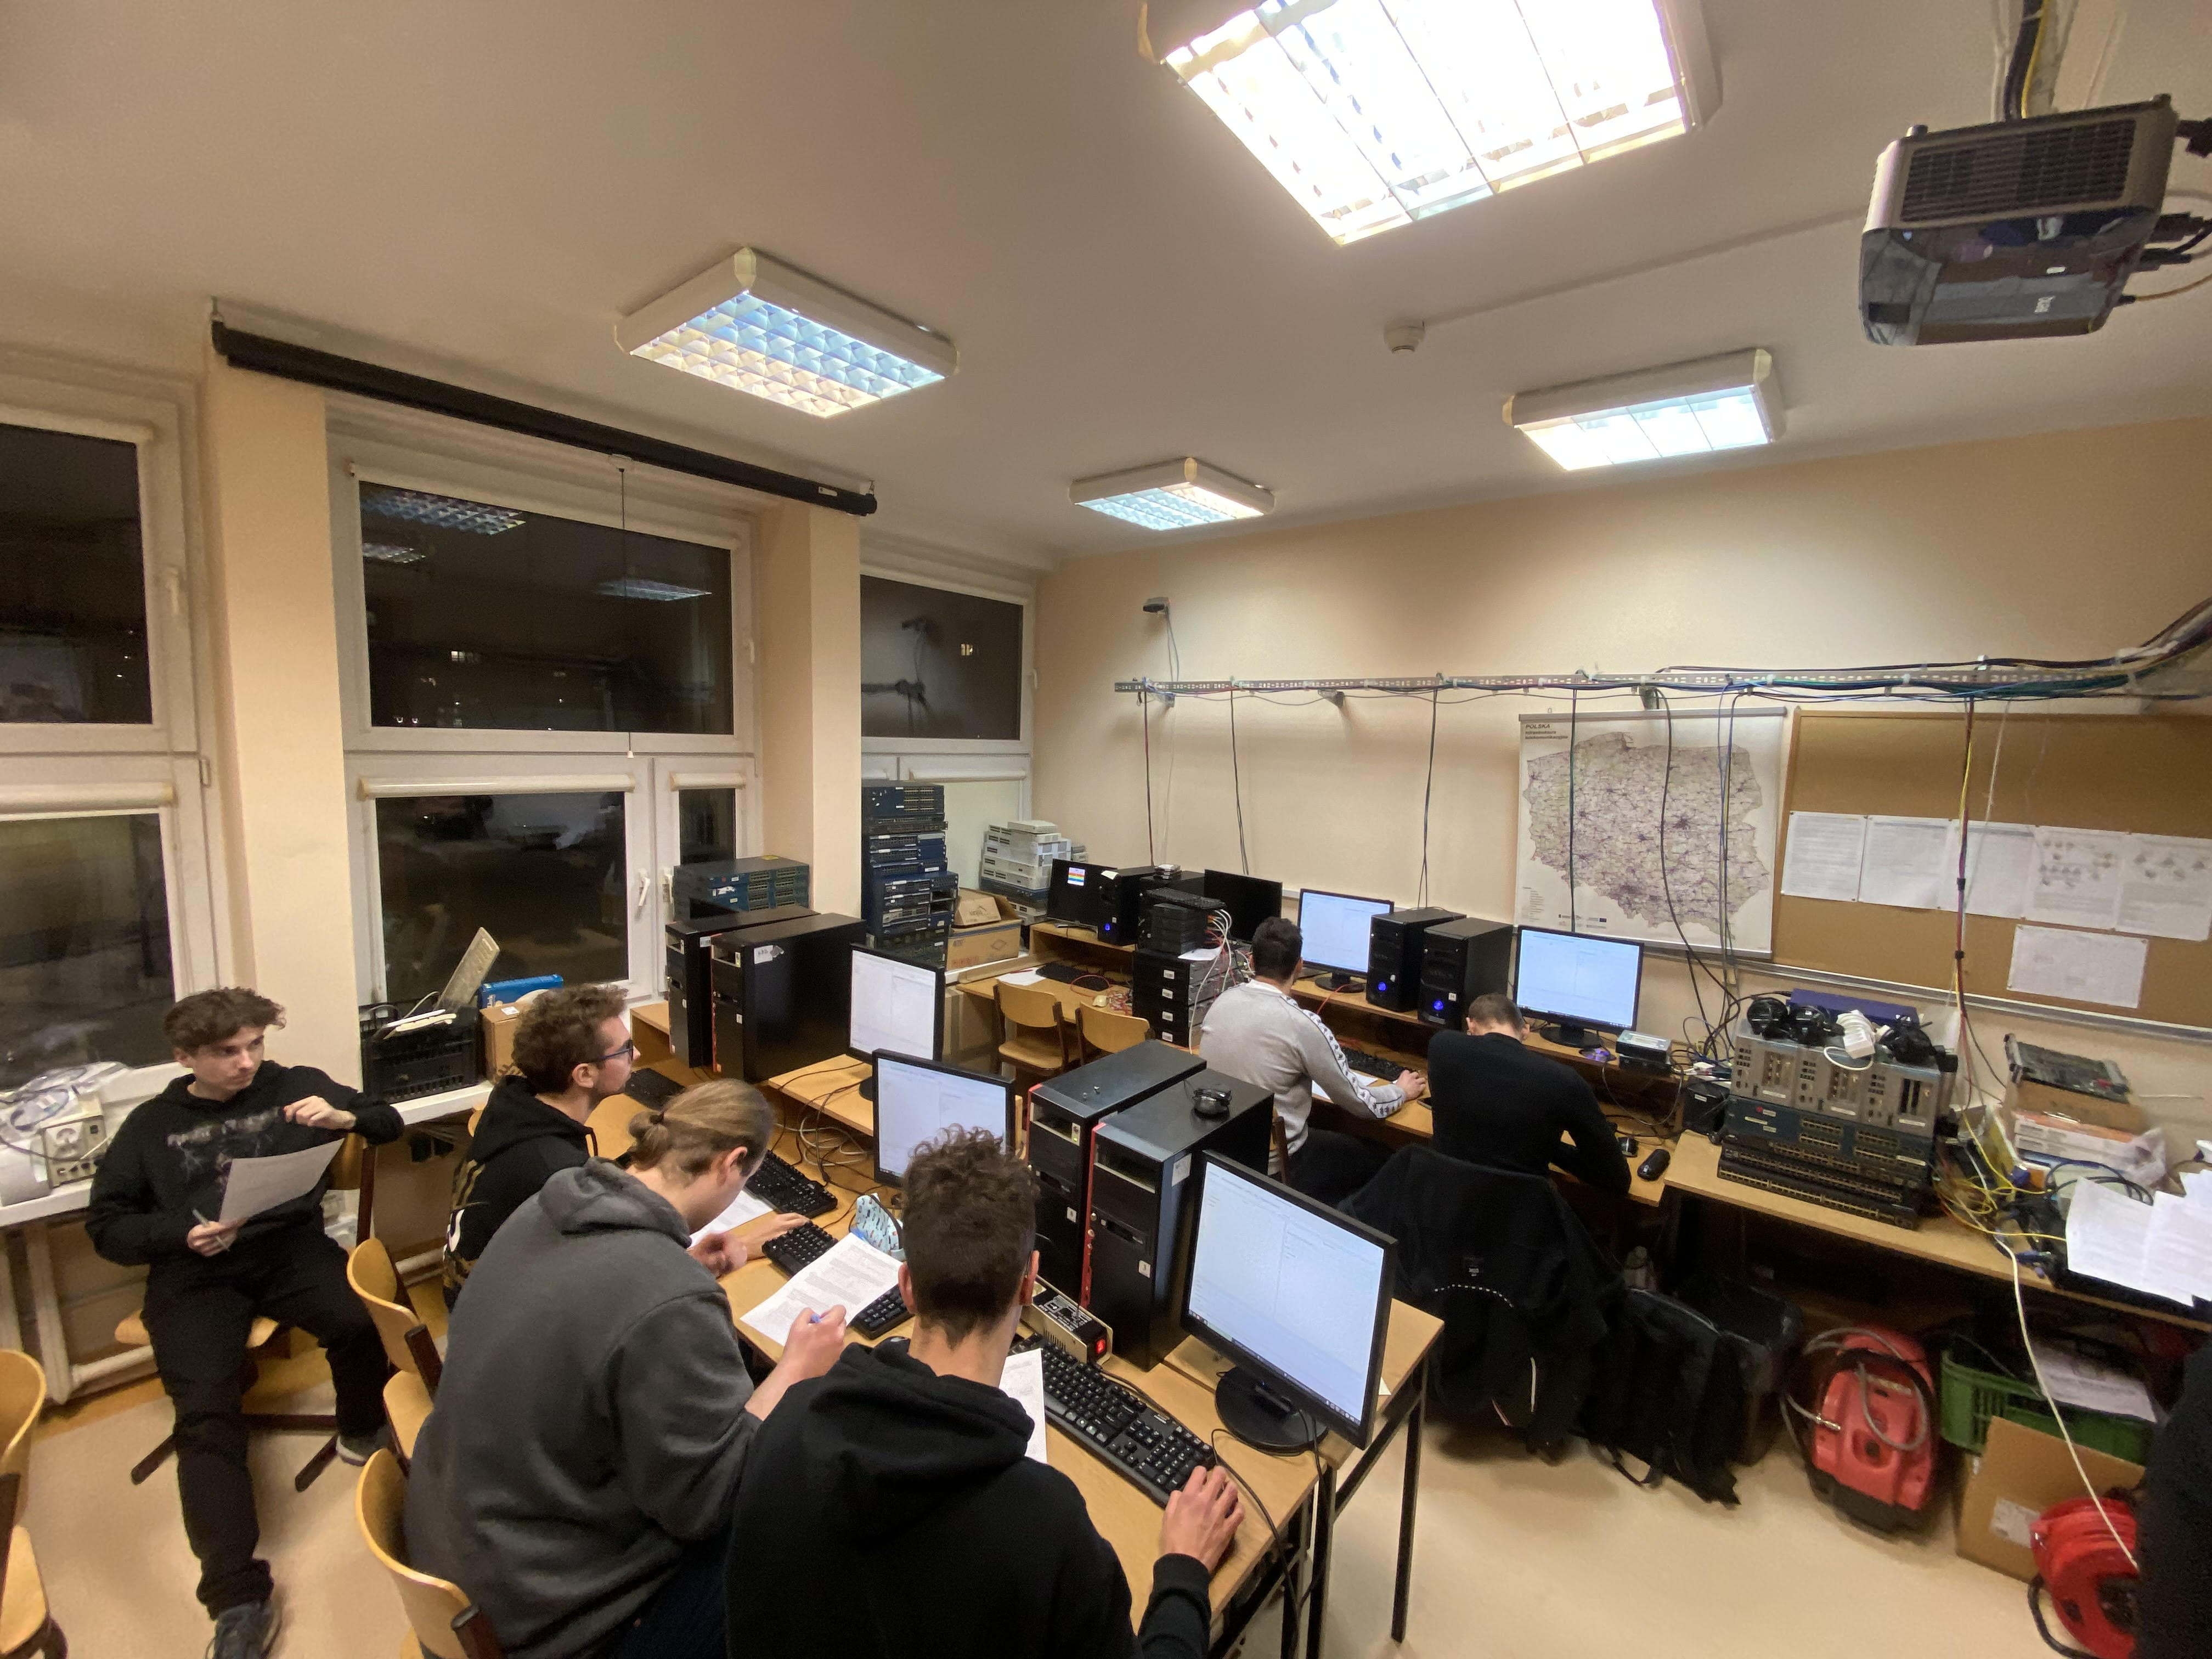
\includegraphics[width=\textwidth]{zajecia_lab.jpg}
    \caption{Zajęcia laboratoryjne przeprowadzone 6 grudnia 2023 r.}
    \label{fig:zajecia_lab_zdjecie}
\end{figure}

Za całość laboratorium studenci mogli uzyskać maksymalnie 4 punkty, w tym: 2 punkty za wejściówkę oraz 2 punkty za zadania laboratoryjne. Prace zostały ocenione w ciągu dwóch dni. 

\subsubsection{Problemy}
Podczas zajęć również napotkano pewne problemy:
\begin{itemize}
    \item Przed zajęciami należało wgrać najnowszą wersję symulatora, jednak przez problemy z dostępem do Internetu okazało się to tak czasochłonne, że zajęcia rozpoczęły się z opóźnieniem około 15 minut,
    \item Studenci znaleźli błąd w symulacji PAM, który został naprawiony przed zajęciami z kolejną grupą.
\end{itemize}

\subsubsection{Wnioski}
Zarówno instrukcja, jak i symulator okazały się zrozumiałe dla studentów mających z nimi styczność pierwszy raz. System operacyjny nie miał żadnego wpływu na pracę studentów, ponieważ całość odbywała się w oknie symulatora. Zadania były wykonywane sprawnie, a poza pytaniami uczestnicy byli w stanie prowadzić dyskusję z prowadzącymi na temat rozwiązań i treści zadań.

Studenci otrzymali bardzo dobre oceny za wykonaną pracę, uśredniając: 95.9\% za całość, 97.2\% za wejściówkę oraz 94.6\% za część laboratoryjną. Spośród zadań na wejściówce jedyne problemy sprawiały zadania 5 i 6, a z zadań laboratoryjnych nieznacznie trudniejsze okazały się zadania związane z kodowaniem Reeda-Solomona.

\section{Podsumowanie}

Wszystkie przyjęte cele pracy zostały osiągnięte, a więc:
\begin{itemize}
    \item stworzono symulator, który umożliwia następujące symulacje:
    \begin{itemize}
        \item symulację sygnału w skrętce z możliwością modyfikacji parametrów wejściowych oraz kanału,
        \item symulację modulacji NRZ, PAM4 oraz PAM16,
        \item symulację kodowania korekcyjnego Reeda-Solomona,
    \end{itemize}
    \item przygotowano instrukcję, wejściówkę oraz zadania laboratoryjne,
    \item przeprowadzono zajęcia dydaktyczne, wykorzystując podane powyżej materiały.
\end{itemize}

Dodatkowym sukcesem można określić intuicyjność symulatora, która była dla autorów istotnym założeniem podczas pracy nad rozwiązaniem. Uczestnicy zajęć nie zgłaszali żadnych problemów w obsłudze programu.

Przy planowaniu celów pracy zrezygnowano, w porozumieniu z promotorem, z pewnych elementów, jednak warto byłoby rozwinąć dyplom o:
\begin{itemize}
    \item symulację skramblowania i deskramblowania,
    \item symulację kodowania LDPC,
    \item symulację przesyłu sygnału światłowodem.
\end{itemize}

\clearpage
\bibliographystyle{unsrt}
\bibliography{references}

\setcounter{secnumdepth}{0}
\section*{Dodatek A: Instrukcja}\label{zajecia-dydaktyczne}
\addcontentsline{toc}{section}{\protect\numberline{}Dodatek A: Zajęcia dydaktyczne}

\subsection{Wejściówka}

Na samym początku zajęć odbędzie się wejściówka składająca się z pytań otwartych
i zamkniętych.
Przykładowe pytania, które mogą znaleźć się na wejściówce to:

\begin{enumerate}
    \item Podaj definicję dodawania i mnożenia w $\mathbb{F}_2$ bądź wypisz wynik tych
    działań dla wszystkich możliwych kombinacji elementów.
    \item Czym się różni słowo kodowe wygenerowane kodem systematycznym i niesystematycznym
    \item Ile błędnych symboli jest w stanie wykryć lub poprawić kod Reeda-Solomona
    \begin{enumerate}[label=\Alph*:]
        \item wykryć: $n-k$, poprawić: $n-k-1$
        \item wykryć: $n-k-1$, poprawić: $n-k-1$
        \item wykryć: $\lfloor \frac{n-k}{2} \rfloor$, poprawić: $\lfloor \frac{n-k}{2} \rfloor$
        \item wykryć: $n-k$, poprawić: $\lfloor \frac{n-k}{2} \rfloor$
    \end{enumerate}
    \item Podaj zaletę oraz wadę stosowania większej ilości poziomów w modulacjach PAM
    \item Czym się różni szerokość pasma od przepustowości?
    \item Opisz krótko czym jest NRZ (Non-Return-to-Zero)
    \item Czym jest przepływność łącza?
\end{enumerate}

\subsection{Narzędzia}

\subsubsection{Symulator - wybór technologii}
Do stworzenia symulatora wybrano język programowania Python i wykorzystano między innymi następujące gotowe rozwiązania:

\begin{enumerate}
    \item PyQt będzie biblioteką wykorzystywaną do stworzenia interfejsu graficznego użytkownika (GUI) dla symulatora. PyQt zapewnia szeroki zakres narzędzi do tworzenia rozbudowanych i przyjaznych użytkownikowi interfejsów, co jest szczególnie ważne w symulatorze dydaktycznym, gdzie interfejs musi być intuicyjny i nie stanowić niepotrzebnego wyzwania lub problemu dla biorących udział w zajęciach,
    \item NumPy jest najpopularniejszą biblioteką Python implementującą algorytmy matematyczne. Między innymi oferuje generatory liczb pseudolosowych o różnych rozkładach, co jest wymagane do prawidłowego generowania ramek ethernetowych i błędów,
    \item  Matplotlib to popularna biblioteka do tworzenia wykresów, przydatna przy tworzeniu wykresów sygnałów,
    \item SPICE (Simulation Program with Integrated Circuit Emphasis) jest powszechnie stosowanym narzędziem do symulacji obwodów elektronicznych. Jest to rozbudowany program, który umożliwia modelowanie i analizę zachowania obwodów złożonych, takich jak układy analogowe, cyfrowe czy mikroelektroniczne. W celu korzystania z tego narzędzia w środowisku Python dostępna jest biblioteka PySpice, będąca interfejsem umożliwiającym korzystanie ze SPICE,
\end{enumerate}

\subsubsection{Interfejs użytkownika}
Interfejs użytkownika został wykonany przy użyciu PyQt5 oraz Qt Designer. Qt Designer to graficzne narzędzie do projektowania interfejsów użytkownika w ramach frameworka Qt. Umożliwia łatwe tworzenie i dostosowywanie wyglądu aplikacji oraz następne jego wygenerowanie jako kodu w języku Python lub C++.

Interfejs składa się z kilku zakładek stworzonych, które umożliwiają przełączanie między częściami aplikacji bez utraty wyników dotychczasowej pracy. Każda zakładka przeznaczona jest do innego zadania laboratoryjnego i zawiera symulacje innych rozwiązań ethernetowych. Podział zadań względem zakładek jest następujący:
\begin{itemize}
    \item Reed-Solomon:
    \begin{itemize}
        \item Kodowanie Reeda-Solomona, zadania: 1, 2, 4,
    \end{itemize}
    \item Reed-Solomon Shift Register:
    \begin{itemize}
        \item Kodowanie Reeda-Solomona, zadanie 3,
    \end{itemize}
    \item PAM16:
    \begin{itemize}
        \item PAM16 w 25GBASE-T / 40GBASE-T, zadanie 1,
    \end{itemize}
    \item PAM:
    \begin{itemize}
        \item modulacje PAM, zadania: 1, 2,
    \end{itemize}
    \item Twisted-pair simulation - narzędzie niewykorzystywane w laboratorium.
\end{itemize}

\begin{figure}[ht]
    \centering
    
\includegraphics{images/zakladki.png}
    \caption{Zakładki symulatora}
    \label{fig:zakladki_image}
\end{figure}

Wykresy są tworzone przy pomocy biblioteki Matplotlib. Została dodatkowo stworzona klasa, która zawiera stworzone wykresy i może być użyta jako element graficznego interfejsu użytkownika, a więc dodana do niego.

\begin{figure}[ht]
    \centering
    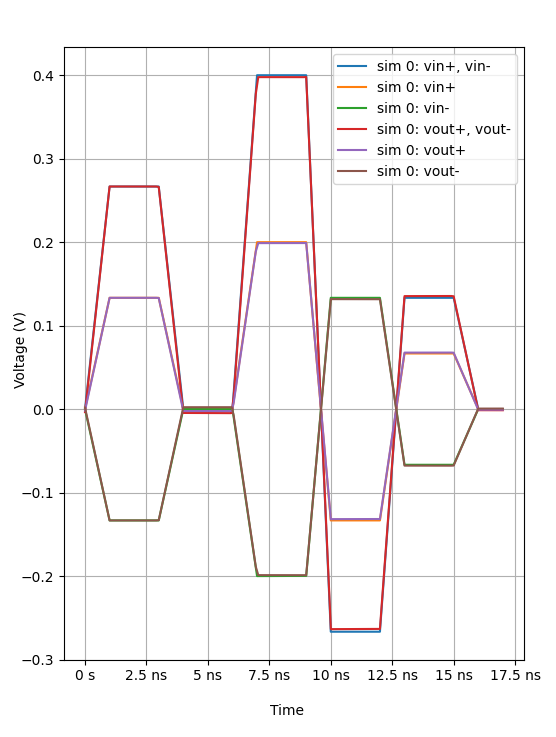
\includegraphics[scale=0.5]{images/wykres.png}
    \caption{Wykres symulacji stworzony przy użyciu Matplotlib}
    \label{fig:wykres_image}
\end{figure}

\subsection{Ćwiczenie dydaktyczne --- modulacje PAM}

W trakcie zajęć laboratoryjnych student będzie miał do dyspozycji symulator phyether, który zawiera implementację wybranych rozwiązań
części standardów 25GBASE-T i 40GBASE-T.

\subsubsection{Wstęp teoretyczny}

Modulacja cyfrowa to technika zamiany bitów na sygnał oraz sygnału na bity. Jest kluczowym zagadnieniem w przesyle danych pomiędzy systemami
komputerowymi. Technologie Ethernetowe wykorzystują wiele technik modulacji. Ćwiczenie te ma na celu przybliżenie oraz porównanie
występujących technik modulacji PAM (Pulse-Amplitude Modulation), która jest jedną z najpopularniejszych w technologii Ethernet.

Najprostszym schematem modulacji jest NRZ --- Non-Return-to-Zero. Chcąc przesłać bit o wartości $0$, na skrętkę zostanie podany sygnał
ujemny, a w przypadku $1$ --- dodatni. Rozwiązanie te niesie za sobą parę wad. Przykładowo, gdy nadawane są długie ciągi zer lub jedynek, sygnał
nie ulega zmianie --- jest to zjawisko niepożądane podczas transmisji i może doprowadzić do desynchronizacji zegarów strony nadawczej i odbiorczej.
Z uwagi na to, NRZ wykorzystywany jest w praktyce w połączeniu z np. kodowaniem liniowym 64b/66b w celu uniknięcia sekwencji zer i jedynek.

PAM jest modulacją, w której dane przesyłane są w postaci zmian amplitudy sygnału. Zmiany te nazywane symbolami. Modulacje PAM różnią się między sobą
liczbą wykorzystywanych poziomów modulacji. PAM3 wykorzystuje trzy poziomy, PAM4 --- cztery, PAM16 --- szesnaście. NRZ można wobec tego nazwać PAM2.
Powodem, dla którego zwiększenie poziomów ma sens jest zwiększona szybkość transmisji. Weźmy na przykład PAM4 --- mając cztery poziomy mamy
do dyspozycji cztery symbole $-3$, $-1$, $1$, $3$, a więc każdy symbol kodować może dwa bity danych. W przypadku NRZ, jeden symbol koduje tylko jeden bit.
Zatem zwiększenie liczby poziomów pozwala na przesył większej ilości bitów przy użyciu jednego symbolu. Schemat ten będzie działał, o ile strona odbiorcza
potrafi rozróżnić poszczególne symbole od siebie, jest to jednak łatwiej osiągalne niż zwiększenie szerokości pasma.
Modulacje PAM4, PAM16 i inne, analogicznie jak NRZ, podatne są na długie ciągi zer i jedynek. Dlatego niezbęde jest zastosowanie różnych metod
zamieniających takie sekwencje na bardziej zróżnicowany ciąg np. skrambler.

\subsubsection{Opis narzędzia}

Program phyether, w zakładce `PAM`, posiada symulator modulacji NRZ, PAM4 oraz PAM16, który ilustruje zachowanie sygnału w skrętce podczas transmisji, w zależności
od wybranych modulacji.

Narzędzie pozwala na:
\begin{itemize}
    \item Wprowadzenie danych w postaci szesnastkowej, które zostaną użyte podczas symulacji
    \item Zamianę wprowadzonych danych na symbole poszczególnych modulacji i dokonanie
        symulacji sygnału w skrętce wykorzystując otrzymane symbole
    \item Wizualizację ww. symualcji
\end{itemize}

Narzędzie będzie wykorzystywane podczas tej części ćwiczenia.

\includegraphics[scale=0.37]{pam_tab.png}

Powyższa grafika prezentuje zakładkę `PAM` programu phyether. Nad przyciskiem \textbf{Simulate} znajduje się pole tekstowe, do którego wpisane mogą być dane w formie
liczb w systemie szesnastkowym. Po wpisaniu danych i kliknięciu \textbf{Simulate}, wpisane dane zamieniane są na symbole modulacji NRZ, PAM4 oraz PAM16, które
następnie wysyłane są na medium. Wynik symulacji przedstawiony jest w dolnej części zakładki.

\subsubsection{Zadania do realizacji}

\begin{enumerate}
    \item Zamień numer swojego indeksu na postać szesnastkową i wykorzystaj go jako liczbę do przesłania. Przeprowadź symulację. Zanotuj w sprawozdaniu
    przybliżony czas transmisji oraz liczbę poziomów natężenia. Opisz wnioski, które nasuwają Ci się po wykonanym ćwiczeniu.
    \item Prześlij ciąg składający się z samych jedynek (fffffff \dots) lub samych zer (000000 \dots). Popatrz na wynik symulacji. Jak nazywa się zaobserwowane zjawisko? Czy znasz sposoby,
    które zapobiegają jego wystąpieniu? Zanotuj w sprawozdaniu.
\end{enumerate}

\subsection{Ćwiczenie dydaktyczne --- PAM16 w 25GBASE-T i 40GBASE-T}
\subsubsection{Wstęp teoretyczny}
Ciekawą kwestią w przypadku modulacji PAM jest także zamiana bitów na konkretne symbole alfabetu modulacji.
Możemy sobie wyobrazić, że w najprostszym przypadku wartość 0 mapowana jest na najmniejszy symbol, natomiast 1111
--- na największy. Istnieją także bardziej wyrafinowane sposoby mapowania, przykładowo popularnym jest zastosowanie kodu Graya.
W tym ćwiczeniu zobaczymy podejście, które zostało zastosowane w standardach 25GBASE-T oraz 40GBASE-T.

Wyżej wymienione standardy korzystają z modulacji PAM16, natomiast symbole nadawane na parach skrętki wybierane są według diagramu
konstelacji DSQ128. Aby wyjaśnić czym on jest, spójrzmy pierw na 64QAM (Quadrature Amplitude Modulation). 64QAM to modulacja, która jest
połączeniem modulacji amplitudy oraz fazy (dane kodowane są poprzez zmianę amplitudy oraz fazy sygnału). Symbole wybierane są na podstawie
diagramu konstelacji 64QAM --- rys.~\ref{fig:lab-64QAM}.

Diagram podzielony jest na cztery części. Oś X odnosi się do fazy, a oś Y --- amplitudy. Każdy symbol, który chcemy nadać,
jest krotką (x, y), która oznacza punkt na diagramie dla danej wartości. Jak można zauważyć, sąsiednie punkty różnią się
między sobą jednym bitem --- dzięki czemu, gdy nastąpi przekłamanie, najprawdopodobniej tylko jeden bit będzie zły.

W standardach 25GBASE-T i 40GBASE-T symbole dobierane są na podstawie diagramu konstelacji DSQ128, który jest złożeniem dwóch
diagramów 64QAM - rys. \ref{fig:lab-dsq128}.

Dane grupowane są w 7-bitowe grupy ($u_0$, $u_1$, $u_2$), ($c_0$, $c_1$, $c_2$, $c_3$), po czym każda taka grupa mapowana jest na krotkę (PAM16$_1$, PAM16$_2$) według algorytmu:

Krok 1:
\begin{align*}
    x_{13} &= \neg u_0 * u_2 \\
    x_{12} &= u_0 \oplus u_2 \\
    x_{11} &= c_0 \\
    x_{10} &= c_0 \oplus c_1 \\
    x_{23} &= (u_1 * u_2) + (u_0 * \neg u_1) \\
    x_{22} &= u_1 \oplus u_2 \\
    x_{21} &= c_2 \\
    x_{20} &= c_2 \oplus c_3
\end{align*}

Krok 2:
\begin{align*}
    x_1 &= 8x_{13} + 4x_{12} + 2x_{11} + x_{10} \\
    x_2 &= 8x_{23} + 4x_{22} + 2x_{21} + x_{20}
\end{align*}

Krok 3:
\begin{align*}
    y_1 &= (x_1 + x_2) \mod 16 \\
    y_2 &= (-x_1 + x_2) \mod 16
\end{align*}

Krok 4:
\begin{align*}
    \text{PAM16}_1 &= 2y_1 - 15 \\
    \text{PAM16}_2 &= 2y_2 - 15
\end{align*}

Symbole są następnie nadawane na kolejnych parach skrętki:
\begin{table}[h]
    \centering
    \resizebox{\textwidth}{!}{%
    \begin{tabular}{c | c c c c c c c |}
        \cmidrule{2-8}
        Pair A & PAM16$_1$<0> & PAM16$_2$<0> & PAM16$_1$<4> & PAM16$_2$<4> & \ldots & PAM16$_1$<508> & PAM16$_2$<508> \\
        \cmidrule{2-8}
        Pair B & PAM16$_1$<1> & PAM16$_2$<1> & PAM16$_1$<5> & PAM16$_2$<5> & \ldots & PAM16$_1$<509> & PAM16$_2$<509> \\
        \cmidrule{2-8}
        Pair C & PAM16$_1$<2> & PAM16$_2$<2> & PAM16$_1$<6> & PAM16$_2$<6> & \ldots & PAM16$_1$<510> & PAM16$_2$<510> \\
        \cmidrule{2-8}
        Pair D & PAM16$_1$<3> & PAM16$_2$<3> & PAM16$_1$<7> & PAM16$_2$<7> & \ldots & PAM16$_1$<511> & PAM16$_2$<511> \\
        \cmidrule{2-8}
    \end{tabular}}
\end{table}

\begin{figure}[h]
    \centering
    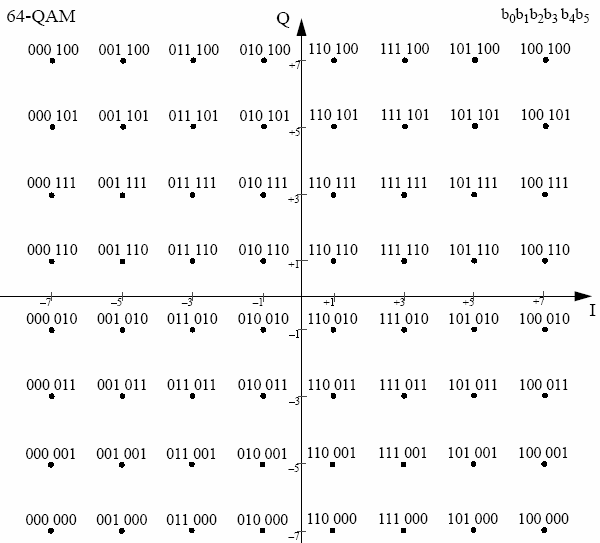
\includegraphics[scale=0.4]{64QAM-constellation-diagram.png}
    \caption{Diagram konstelacji 64QAM}
    \label{fig:lab-64QAM}
\end{figure}

\begin{figure}[h]
    \centering
    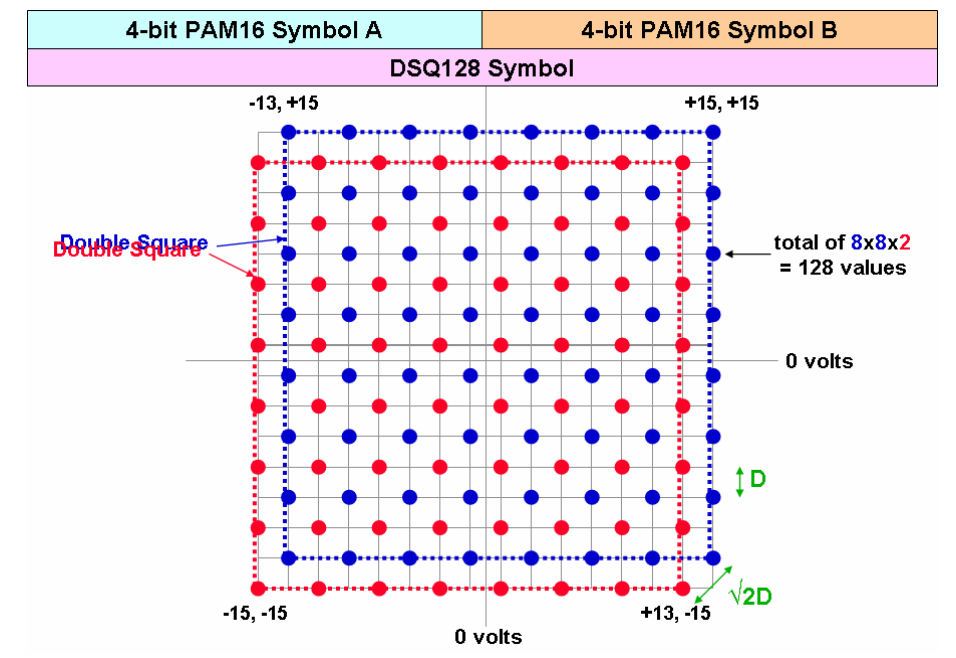
\includegraphics[scale=0.4]{dsq128.png}
    \caption{Diagram konstelacji DSQ128}
    \label{fig:lab-dsq128}
\end{figure}

\clearpage

\subsubsection{Opis narzędzia}

\begin{figure}[ht]
    \centering
    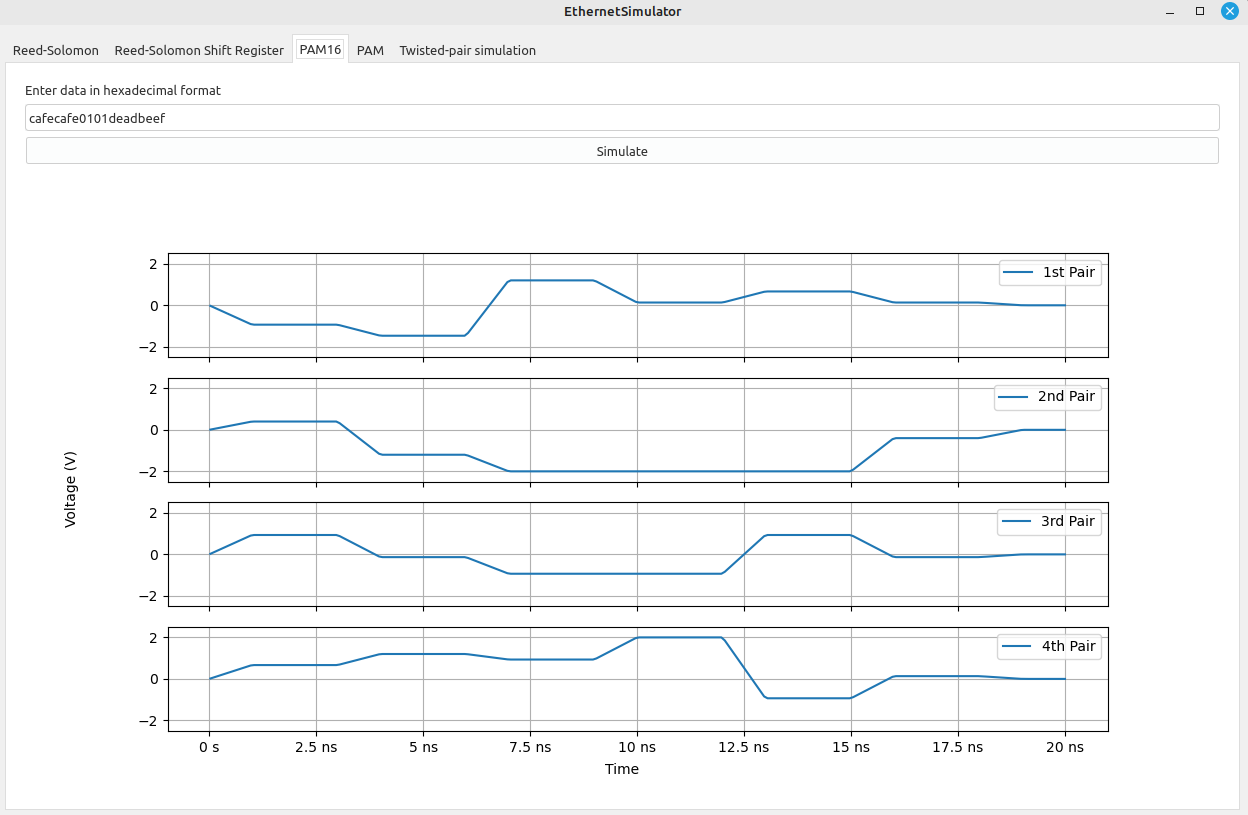
\includegraphics[width=\textwidth]{pam16-tab.png}
    \caption{Zakładka PAM16}
    \label{fig:zakladka_pam16}
\end{figure}

Program phyether, w zakładce `PAM16`, posiada symulator modulacji PAM16 standardu 25GBASE-T / 40GBASE-T, który ilustruje zachowanie
sygnału w skrętce podczas transmisji na podstawie wprowadzonych danych.

Narzędzie pozwala na:
\begin{itemize}
    \item Wprowadzenie danych w postaci szesnastkowej, które zostaną użyte podczas symulacji
    \item Zamianę wprowadzonych danych na symbole DSQ128 i przeprowadzenie symulacji sygnału na czterech parach skrętki 
        wykorzystując otrzymane symbole
    \item Wizualizację ww. symualcji
\end{itemize}

Narzędzie będzie wykorzystywane podczas tej części ćwiczenia.

\clearpage

\subsubsection{Zadania do realizacji}

\begin{enumerate}
    \item Zastosowanie DSQ128 nie eliminuje możliwości wystąpienia stałej składowej. Znajdź ciąg, który
    temu dowodzi i zanotuj go w sprawozdaniu.
\end{enumerate}

\subsection{Ćwiczenie dydaktyczne --- Kodowanie Reeda-Solomona}

\subsubsection{Wstęp teoretyczny}
Kodowanie korekcyjne Reeda-Solomona zostało stworzone przez Irvina S. Reeda
oraz Gustava Solomona w 1960 roku.
Kody Reeda-Solomona charakteryzują się kilkoma parametrami:
\begin{itemize}
    \item alfabetem w ciele skończonym $\mathbb{F}_{2^m}$, $m>1$
    \item długością wiadomości $k$ do zakodowania $k < 2^{m}$
    \item długością słowa kodowego $n$ gdzie $k < n < 2^{m}$
    \item wielomianem generującym $g(x)$
\end{itemize}

Kody Reeda-Solomona cechują się możliwością korekty $\lfloor \frac{n-k}{2} \rfloor$
lub wykrycia $n-k$ błędnych symboli. Symbol w ciele $\mathbb{F}_{2^m}$ składa się
z $m$ bitów co w przypadku błędów grupowych daje możliwość korekty maksymalnie
$m \cdot \lfloor \frac{n-k}{2} \rfloor$ bitów bądź detekcji $m(n-k)$ przekłamanych bitów

Aby zrozumieć działanie kodu Reeda-Solomona trzeba najpierw zrozumieć
czym jest ciało skończone $\mathbb{F}_q$ zwane też ciałem Galois $\operatorname{GF}(q)$.

\paragraph{Ciało skończone $\mathbb{F}_q$}

Ciało to jest ciałem $K$ rzędu $q$ czyli takie które zawiera jedynie $q$ elementów. Aby ciało skończone istniało $q$ musi spełniać warunek $q=p^k$, $k \in \{ 1, 2, \ldots \}$ gdzie $p$ jest liczbą pierwszą oraz definiować działania dodawania i mnożenia spełniające kilka warunków:
\begin{itemize}
    \item dodawanie i mnożenie jest łączne, przemienne oraz zawiera elementy neutralne
    \item każdy element musi posiadać element odwrotny względem dodawania
    \item każdy element oprócz $0$ musi posiadać element odwrotny względem mnożenia
    \item mnożenie jest rozdzielne względem dodawania
\end{itemize}

Aby stworzyć ciało $\mathbb{F}_p$ gdzie $p$ jest liczbą pierwszą można wykorzystać pierścień klas reszt $\modulo{p}$ w którym działania to zwykłe dodawanie i mnożenie modulo
\begin{align*}
    \modulo{p} = \{ [a]_p \; | \; a \in \mathbb{Z} \} &= \{ [0]_p, [1]_p,
    [2]_p, \ldots, [p-1]_p \} \\
    [a]_p + [b]_p &= [a + b]_p \\
    [a]_p \cdot [b]_p &= [a \cdot b]_p
\end{align*}

W tym wprowadzeniu będą używane jedynie ciała $\mathbb{F}_2$ oraz $\mathbb{F}_{2^m}$ z których korzysta kod Reeda-Solomona.

\paragraph{Ciało $\mathbb{F}_2$}

Ciało $\mathbb{F}_2$ jest jednym z najczęściej używanych ciał w informatyce. Ciało to definiuje 2 elementy $\{ 0, 1 \}$ w którym działania $+$ i $\cdot$ są równoważne operacjom logicznym XOR oraz AND
\begin{table}[H]
    \captionof*{table}{Dodawanie i mnożenie w $\mathbb{F}_2$}
    \centering
    \begin{tabular}{c c | c c}
        \toprule
        a & b & $+$ & $\cdot$ \\
        \midrule
        0 & 0 & 0 & 0 \\
        \midrule
        0 & 1 & 1 & 0 \\
        \midrule
        1 & 0 & 1 & 0 \\
        \midrule
        1 & 1 & 0 & 1 \\
        \bottomrule
    \end{tabular}
\end{table}


\paragraph{Ciało $\mathbb{F}_{2^m}$}

Aby zdefiniować ciało skończone $\mathbb{F}_{2^m}$ potrzebujemy najpierw
znaleźć wielomian nierozkładalny $p(x)$ stopnia $m$, czyli taki który nie
da się przedstawić jako iloczyn dwóch innych wielomianów stopnia
mniejszego $p(x) = g(x) \cdot f(x)$

Wielomian jest ten potrzebny do zdefiniowania działania mnożenia ponieważ elementy tego ciała interpretowane są jako wielomiany w postaci:
\begin{align*}
    \sum_{n=0}^{m-1} c_n \alpha^n = c_{0} + c_{1}\alpha + c_{2}\alpha^{2} + \cdots + c_{m-1}\alpha^{m-1},
    c_{n} \in \mathbb{F}_2
\end{align*}

Wielomiany te mogą być reprezentowane jako liczby binarne $c_{m-1} c_{m-2} \ldots c_{1} c_{0}$ bądź po konwersji liczby binarnej jako np.\ liczby dziesiętne. Przykładowe wielomiany w ciele $\mathbb{F}_{2^4}$ i ich różne zapisy podane są w tabelce:
\begin{table}[hp]
    \captionof*{table}{Interpretacje niektórych elementów ciała $\mathbb{F}_{2^4}$}
    \centering
    \begin{tabular}{c c c}
        \toprule
        Wielomian & Liczba Binarna & Liczba dziesiętna \\
        \midrule
        $x^3 + x^2 + x + 1$ & 1111 & 15 \\
        \midrule
        $x^3 + x$ & 1010 & 9 \\
        \midrule
        $x + 1$ & 11 & 3 \\
        \bottomrule
    \end{tabular}
\end{table}

Dodawanie elementów w ciele $\mathbb{F}_{2^m}$ jest po prostu zwykłym dodawaniem wielomianów, trzeba tylko pamiętać, że współczynniki dodajemy w ciele $\mathbb{F}_2$ czyli XORujemy:
\begin{align*}
    \sum_{n=0}^{m-1} c_n \alpha^n + \sum_{n=0}^{m-1} d_n \alpha^n =
    \sum_{n=0}^{m-1} (c_n + d_n) \alpha^n
\end{align*}
Wynikiem mnożenia $a$ i $b$ w ciele $\mathbb{F}_{2^m}$ jest reszta z
dzielenia iloczynu tych wielomianów przez wielomian nierozkładalny $p(x)$.
Dzielenie jak i mnożenie można wykonać tak jak na zwykłych wielomianach, pamiętając o tym, że współczynniki są w ciele $\mathbb{F}_2$.
\newline
Przykładowe działanie mnożenia w $\mathbb{F}_{2^2}$, wielomian nierozkładalny $p(x)=x^2 + x + 1$

\begin{align*}
    a &= \alpha + 1 \text{, } b = \alpha + 1 \\
    a \cdot b &= (\alpha + 1)^2 &\mod x^2 + x + 1 \\
    a \cdot b &= \alpha^2 + [2]_{2}x + 1 &\mod x^2 + x + 1 \\
    a \cdot b &= \alpha^2 + 1 &\mod x^2 + x + 1 \\
    a \cdot b &= \alpha
\end{align*}

Zamiast liczenia reszty z dzielenia można także skorzystać z pewnej zależności. Zdefiniujmy $\alpha$ jako pierwiastek wielomianu $p(x)$.
\begin{align*}
    [-1]_2 &\equiv [1]_2 \\
    p(\alpha) &= 0 \\
    \alpha^2 + \alpha + 1 &= 0 \\
    \alpha^2 &= -\alpha - 1 \\
    \alpha^2 &= \alpha + 1
\end{align*}

Teraz zamiast liczyć resztę z dzielenia możemy po prostu podstawić $\alpha^2$:
\begin{align*}
    a \cdot b &= \alpha^2 + 1 \\
    a \cdot b &= (\alpha + 1) + 1 \\
    a \cdot b &= \alpha
\end{align*}

\paragraph{Oryginalny kod Reeda-Solomona}
Sposób kodowania przedstawiony w pracy Reeda i Solomona polega na stworzeniu wielomianu $p_m(x)=\sum_{i=0}^{k-1}m_{i}x^i$, gdzie $m_i\in\mathbb{F}_{2^m}$
to $i$\nobreakdash-ty element wiadomości, po czym za pomocą tego wielomianu
obliczane jest słowo kodowe $C(m)=(p_m(a_0), p_m(a_1), \ldots, p_m(a_{n-1}))$
gdzie $a_i$ to różne elementy ciała $\mathbb{F}_{2^m}$.
\newline
Przykładowy kod RS dla $\mathbb{F}_{2^2}$, $p(x) = x^2 + x + 1$, $n=3$,
$k=2$, wiadomość to 2 liczby 2 i 3.

\begin{align*}
    p_m(x) &= 3x + 2 \\
    p_m(0) &= 3 \cdot 0 + 2 = 2 \\
    p_m(1) &= 3 \cdot 1 + 2 = 3 + 2 = 0\text{b}11 + 0\text{b}10 = 0\text{b}01 = 1 \\
    p_m(2) &= 3 \cdot 2 + 2 = (\alpha + 1) \cdot \alpha + \alpha \\
    p_m(2) &= 3 \cdot 2 + 2 = \alpha^2 + \alpha + \alpha = \alpha + 1 = 3 \\
    p_m(3) &= 3 \cdot 3 + 2 = (\alpha + 1)^2 + \alpha = \alpha + \alpha = 0
\end{align*}

Zakodowana wiadomość to ``2 1 3 0''

\paragraph{Kod systematyczny}

Za pomocą niewielkiej modyfikacji można stworzyć kod systematyczny czyli taki w którym słowo kodowe zawiera w sobie kodowaną wiadomość.
Żeby stworzyć kod systematyczny musimy zmodyfikować sposób tworzenia wielomianu w taki sposób by $p_m(x_i)=m_i$ dla $i \in \{0,1,\ldots,k-1\}$.

Jednym ze sposobów stworzenia takiego wielomianu jest użycie metody interpolacji wielomianów. Słowo kodowe wygenerowane z tego wielomianu będzie zawierało wiadomość w pierwszych $k$ elementach.
\[C(m)=(p_m(a_0), p_m(a_1), \ldots, p_m(a_{n-1}))=(m_0, m_1, \ldots, m_{k-1}, p_m(a_k), p_m(a_{k+1}), \ldots, p_m(a_{n-1}))\]

\paragraph{kod BCH}

Kody BCH~(Bose-Chaudhuri-Hocquenghem) są kodami cyklicznymi co oznacza że każde przesunięcie słowa kodowego jest także słowem kodowym np.
\begin{align*}
    (c_0, c_1,\ldots, c_{n-2}, c_{n-1})\text{, }(c_{n-1}, c_0, \ldots, c_{n-3}, c_{n-2})
\end{align*}

Aby zbudować kod BCH Reeda-Solomona potrzebujemy najpierw funkcji minimalnej pierwiastka $\alpha$, czyli takiego minimalnego wielomianu nierozkładalnego $p(x)$ stopnia $m$ dla którego istnieje element prymitywny~(pierwiastek) $\alpha$ który pozwala wygenerować całe ciało skończone
\begin{align*}
    \mathbb{F}_{2^m} = \{0, 1, \alpha, \alpha^2, \ldots, \alpha^{p^{m}-1} \}
\end{align*}

Mając taki element prymitywny jesteśmy w stanie stworzyć wielomian generujący $g(x)$ używając wzoru
\begin{align*}
    t &= n - k \\
    g(x) = \prod_{i=0}^{t-1} (x - \alpha^i) &= g_{t}x^t + g_{t-1}x^{t-1} +
    \cdots + g_{1}x + g_{0}
\end{align*}
Aby utworzyć słowo kodowe wystarczy pomnożyć wielomian $p_m(x)$ przez wielomian generujący $g(x)$

\paragraph{systematyczny kod BCH}\label{systematic-bch-rs}

Aby uzyskać systematyczne słowo kodowe $s(x)$ musimy obliczyć:
\begin{align*}
    s_r(x) &= p_m(x) \cdot x^t \mod g(x) \\
    s(x) &= p_m(x) \cdot x^t - s_r(x)
\end{align*}

\subsubsection{Narzędzia}
\paragraph{Reed-Solomon}
\begin{center}
    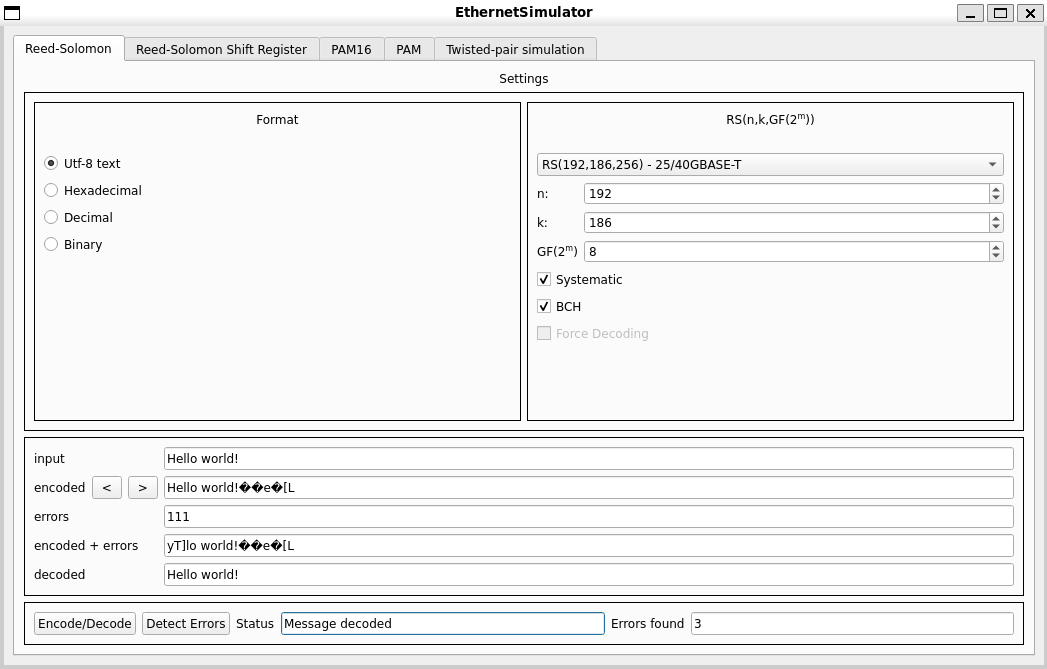
\includegraphics[width=0.95\textwidth,keepaspectratio]{rs-tab.png}
\end{center}
Narzędzie pozwala na:
\begin{itemize}
    \item Kodowanie i dekodowanie wiadomości różnymi koderami o różnych
    parametrach
    \item Nakładanie na zakodowaną wiadomość błędów w celu przetestowania
    możliwości detekcji i korekty błędów przez kod Reeda-Solomona
    \item Zmianę formatu symboli w celu łatwiejszego zobrazowania co się
    dzieje w poszczególnych etapach
\end{itemize}

Zakładka Reed-Solomon składa się z 3 części
\begin{itemize}
    \item Format --- pozwala na zmianę formatu wyświetlanych danych.
    Tryb tekstowy pozwala na szybkie zorientowanie się jak dane się
    zmieniają. Tryb binarny pozwoli na dokładne dodanie błędów do
    słowa kodowego. Kodowanie znaków tekstowych to UTF-8 w związku z
    czym polskie znaki diakrytyczne kodowane są na 2 bajtach.
    \item RS($n$, $k$, $GF(2^m)$) --- parametry kodu
    RS~(wielomian $p(x)$ jest obliczany automatycznie).
    \item Dane --- tutaj możemy wpisać wiadomość którą chcemy
    zakodować lub błędy które będą XORowane ze słowem kodowym oraz
    zobaczyć wynik kodowania. Status informuje nas o tym czy
    znaleziono błędy bądź czy udało się zdekodować wiadomość.
    `Errors found' informuje ile błędów zostało poprawionych.
\end{itemize}

Tryb tekstowy nie jest w stanie poprawnie wyświetlić wszystkich
znaków, część jest zamieniana na znaki zapytania a część jest tzw.
~znakami białymi (spacje, tabulatory bądź znaki niewyświetlane).
Strzałki przy `encoded' pozwalają na przesunięcie symboli w lewo i prawo.

\paragraph{Reed-Solomon Shift Register}
\begin{center}
    \includegraphics[width=0.95\textwidth,keepaspectratio]{rs-register-tab.png}
\end{center}
Narzędzie pozwala na:
\begin{itemize}
    \item Obliczanie wielomianu generującego kod Reeda-Solomona
    \item Zobrazowanie jak działa przykładowy koder Reeda-Solomona
    \item Zaznajomienie się z reprezentacją w postaci wielomianowej symboli z ciała $\mathbb{F}_{2^m}$
\end{itemize}

W tej zakładce koder RS zaimplementowany został zgodnie z modelem
funkcyjnym udostępnionym w standarcie Ethernet. Po przejściu
wszystkich symboli wiadomości element `Switch' zacznie przepuszczać symbole parzystości.
W opcjach po lewej możemy podobnie jak w poprzedniej zakładce wybrać
parametry kodera oraz dodatkowo wybrać inne wielomiany i elementy prymitywne. Przycisk `Calculate generating polynomial' obliczy
wielomian generujący a `Calculate primitive poly/ement' obliczy element i wielomian prymitywny dla podanego ciała skończonego $\mathbb{F}_{2^m}$.
Po prawej stronie mamy dane wejściowe oraz aktualny stan rejestrów $p_i$. `Fill symbol' jest symbolem który będzie wysyłany jeżeli zabraknie symboli na wejściu.

\subsubsection{Zadania}

\begin{itemize}
    \item Zakładka: Reed-Solomon, ustawienia programu: kod systematyczny BCH, $n=15$, $GF=2^4$.
    Dla $k \in \{ 2, 6, 10, 13 \}$ sprawdź wartość słowa kodowego dla k-symbolowej wiadomości zawierającej same zera. Dlaczego otrzymałeś takie słowa kodowe?
    \item Zakładka: Reed-Solomon, ustawienia programu: $n = 7$, $k = 3$, $GF = 2^3$,
    kod systematyczny BCH, tryb dziesiętny, wiadomość wejściowa `1 2 3'.
    Sprawdź dla błędów `3', `3 2', `3 2 1' oraz `3 2 1 4' czy dekoder jest w stanie
    wykryć błędy oraz czy jest w stanie je poprawić a jeżeli tak to czy poprawnie.
    Czy wiesz dlaczego pojawiły się rozbieżności między błędami poprawionymi a wykrytymi?
    \item Zakładka: Reed-Solomon Shift Register, ustawienia programu:
    $n = 3$, $k = 2$, $GF = 2^2$. Oblicz wielomiany prymitywne naciskając przycisk
    `Calculate primitive poly/element'.
    Zakoduj wiadomość: `2 1' w symulatorze po czym zakoduj wiadomość
    używając wzoru z sekcji `Systematyczny kod BCH'. Porównaj wyniki.
    \item Zakładka: Reed-Solomon, ustawienia programu: $n = 15$, $k=7$, $GF = 2^4$,
    kod systematyczny BCH.
    Zakoduj dowolną niezerową $k$-symbolową wiadomość. Sprawdź czy przesunięcia słowa kodowego
    (z użyciem strzałek przy słowie `encoded') także będą słowem kodowym.
\end{itemize}


\setcounter{secnumdepth}{0}
\section*{Dodatek B: Wejściówka}
\addcontentsline{toc}{section}{\protect\numberline{}Dodatek B: Wejściówka}

\begin{enumerate}
    \item Która biblioteka wykorzystywana jest do stworzenia GUI?
    \begin{enumerate}[label=\Alph*)]
        \item Tkinter
        \item PyQT5
        \item OpenGL
        \item WindowsForms
    \end{enumerate}

    \item Ile błędnych symboli jest w stanie wykryć lub poprawić kod Reeda-Solomona?
    \begin{enumerate}[label=\Alph*)]
        \item wykryć: $n-k$, poprawić: $n-k-1$
        \item wykryć: $n-k-1$, poprawić: $n-k-1$
        \item wykryć: $\lfloor \frac{n-k}{2} \rfloor$, poprawić: $\lfloor \frac{n-k}{2} \rfloor$
        \item wykryć: $n-k$, poprawić: $\lfloor \frac{n-k}{2} \rfloor$
    \end{enumerate}
    \item Podaj zaletę oraz wadę stosowania większej ilości poziomów w modulacjach PAM.\\ \\ \\ \\ \\
    \item Opisz krótko czym jest NRZ (Non-Return-to-Zero).\\ \\ \\ \\
    \item Podaj definicję dodawania i mnożenia w $\mathbb{F}_2$ bądź wypisz wynik tych działań dla wszystkich możliwych kombinacji elementów.
    działań dla wszystkich możliwych kombinacji elementów.\\ \\ \\ \\ \\
    \item Czym się różni słowo kodowe wygenerowane kodem systematycznym i niesystematycznym?
\end{enumerate}


\setcounter{secnumdepth}{0}
\section*{Dodatek C: Zadania laboratoryjne}
\addcontentsline{toc}{section}{\protect\numberline{}Dodatek C: Zadania laboratoryjne}

\begin{enumerate}
    \item Zakładka: Reed-Solomon, ustawienia programu: kod systematyczny BCH, $n=15$, $GF=2^4$.
    Dla $k \in \{ 2, 6, 10, 13 \}$ sprawdź wartość słowa kodowego dla k-symbolowej wiadomości zawierającej same zera. Dlaczego otrzymałeś takie słowa kodowe?\\ \\ \\ \\ \\ \\ \\
    
    \item Zakładka: Reed-Solomon, ustawienia programu: $n = 7$, $k = 3$, $GF = 2^3$, tryb dziesiętny, wiadomość wejściowa: "1 2 3",
    kod systematyczny BCH. Wpisz wiadomość do zakodowania. Sprawdź i zapisz, ile błędnych symboli koder jest w stanie poprawić i wykryć.
    \begin{table}[h]
    \renewcommand{\arraystretch}{1.8}
    \centering
    \begin{tabular}{|c|c|c|>{\centering\arraybackslash}p{5cm}|}
        \hline
        \textbf{Błąd} & \textbf{Wykryto} & \textbf{Poprawiono} & \textbf{Ile} \\
        \hline
        "3" & & & \\
        \hline
        "3 2" & & & \\
        \hline
        "3 2 1" & & & \\
        \hline
    \end{tabular}
    \label{tab:rs2}
\end{table}
    \item Zakładka: Reed-Solomon Shift Register, ustawienia programu: $n = 7$, $k = 3$, $GF = 2^3$. Oblicz wielomiany prymitywne automatycznie naciskając przycisk `Calculate primitive poly/element'.
    Zakoduj i zapisz 3 dowolne niezerowe wiadomości.
    Przejdź do zakładki Reed-Solomon i powtórz działania używając tych samych wiadomości oraz używając kodera systematycznego BCH z tymi samymi $n$, $k$, $GF$.\\ \\ \\ \\
    \item Zakładka: Reed-Solomon, ustawienia programu: kod systematyczny BCH, $n=7$, $k=2$, $GF=2^3$.
    Oblicz słowo kodowe dla wiadomości składającej się z liczb dziesiętnych `3 1'.
    Zwiększ $k$ o 1 i dodaj k-ty symbol ze słowa kodowego do wiadomości. Powtarzaj aż do $k=6$.
    Zapisz słowa kodowe i zanotuj spostrzeżenia.
    Czy wiesz, dlaczego otrzymałeś takie słowa kodowe?
    
\begin{table}[h]
    \renewcommand{\arraystretch}{1.8}
    \centering
    \begin{tabular}{|c|>{\centering\arraybackslash}p{12cm}|}
        \hline
        \textbf{k} & \textbf{Słowo kodowe} \\
        \hline
        1 & \\
        \hline
        2 & \\
        \hline
        3 & \\
        \hline
        4 & \\
        \hline
        5 & \\
        \hline
        6 & \\
        \hline
    \end{tabular}
    \label{tab:rs4}
\end{table}
\newpage
\item Zamień numer swojego indeksu na postać szesnastkową i wykorzystaj go jako liczbę do przesłania. Przeprowadź symulację. Zanotuj w sprawozdaniu
przybliżony czas transmisji oraz liczbę poziomów natężenia. Opisz wnioski, które nasuwają Ci się po wykonanym ćwiczeniu. \\ \\ \\ \\ \\ \\ \\ \\ \\ \\ \\ \\ \\ \\ \\
\item Prześlij ciąg składający się z samych jedynek (fffffff \dots). Popatrz na wynik symulacji. Jak nazywa się zaobserwowane zjawisko? Czy znasz sposoby,
które zapobiegają jego wystąpieniu? Zanotuj w sprawozdaniu.
\end{itemize}

\setcounter{secnumdepth}{0}
\section*{Dodatek D: Kod źródłowy symulatora}
\addcontentsline{toc}{section}{\protect\numberline{}Dodatek D: Kod źródłowy symulatora}

Kod źródłowy programu dostępny jest na załączonym urządzeniu przenośnym oraz pod adresem: https://github.com/iwanicki92/Ethernet-physical-layer-simulator/tree/dev.

\setcounter{secnumdepth}{0}
\section*{Dodatek E: Instrukcja instalacji symulatora}
\addcontentsline{toc}{section}{\protect\numberline{}Dodatek E: Instrukcja instalacji symulatora}

\subsection{Z dostępem do Internetu}
W przypadku dostępu do Internetu wystarczy zainstalować wersję języka Python spełniającą warunek: $3.9 <= wersja <= 3.11$ oraz uruchomić polecenie instalacji symulatora: \\ pip install git+https://github.com/iwanicki92/Ethernet-physical-layer-simulator.git@dev

\subsection{Bez dostępu do Internetu}
W przypadku braku dostępu do Internetu konieczne jest skopiowanie zawartości specjalnie przygotowanego do tej okazji urządzenia przenośnego dołączonego do pracy. Zawiera on gotowe środowisko pythonowe oraz kod źródłowy symulatora.

\setcounter{secnumdepth}{0}
\section*{Dodatek F: Rozwiązania zadań}
\addcontentsline{toc}{section}{\protect\numberline{}Dodatek F: Rozwiązania zadań}

\subsection*{Rozwiązania wejściówki}
\begin{enumerate}
    \item Podaj definicję dodawania i mnożenia w $\mathbb{F}_2$ bądź wypisz wynik tych
    działań dla wszystkich możliwych kombinacji elementów.
    \begin{itemize}
        \item Odpowiedź: dodawanie to XOR a mnożenie to AND. Pozostałe możliwe odpowiedzi to Tablica~\ref{truth_table:title} bądź~(\ref{modulo_addition})
        oraz~(\ref{modulo_multiplication})
    \end{itemize}
    \item Czym się różni słowo kodowe wygenerowane kodem systematycznym i niesystematycznym
    \begin{itemize}
        \item Odpowiedź: słowo kodowe w kodowaniu systematycznym w przeciwieństwie do niesystematycznego zawiera w sobie kodowaną wiadomość, sekcja~\ref{subsection:Kod systematyczny}
    \end{itemize}
    \item Ile błędnych symboli jest w stanie wykryć lub poprawić kod Reeda-Solomona?
    \begin{itemize}
        \item Odpowiedź: wykryć: $n-k$, poprawić: $\lfloor \frac{n-k}{2} \rfloor$, sekcja~\ref{subsection:wlasciwosci}
    \end{itemize}
    \item Podaj zaletę oraz wadę stosowania większej ilości poziomów w modulacjach PAM.
    \begin{itemize}
        \item Odpowiedź: \\
        Zaleta:
        \begin{itemize}
            \item większa przepustowość bez zwiększania szerokości pasma.
        \end{itemize}
        Wady:
        \begin{itemize}
            \item zmniejszony stosunek sygnału do szumu,
            \item większa podatność na zakłócenia,
            \item konieczność używania dokładniejszych urządzeń.
        \end{itemize}
    \end{itemize}
    \item Opisz krótko czym jest NRZ (Non-Return-to-Zero).
    \begin{itemize}
        \item Odpowiedź: rodzaj kodowania o dwóch poziomach - dla 0 sygnał ujemny, dla 1 sygnał dodatni.
    \end{itemize}
\end{enumerate}

\subsection*{Rozwiązania ćwiczeń}
\begin{enumerate}
    \item Zakładka: Reed-Solomon, ustawienia programu: kod systematyczny BCH, $n=15$, $GF=2^4$.
    Dla $k \in \{ 2, 6, 10, 13 \}$ sprawdź wartość słowa kodowego dla k-symbolowej wiadomości zawierającej same zera. Dlaczego otrzymałeś takie słowa kodowe? \\ \\
    Odpowiedź: Otrzymaliśmy same zera ponieważ według wzoru z sekcji~\ref{subsubsection:systematic-bch} dla $p_m(x) = 0$ zawsze dostaniemy zera
    \begin{align*}
        c_r(x) &= 0 \cdot x^t \mod g(x) \\
        c_r(x) &= 0 \mod g(x) \\
        c_r(x) &= 0 \\
        c(x) &= 0 \cdot x^t - 0 \\
        c(x) &= 0
    \end{align*}

    Odpowiedź 2: Kod BCH jest kodem systematycznym dlatego pierwsze $k$ symboli
    także będzie miało zera. Aby obliczyć pozostałe $n-k$ symboli musimy mnożyć
    i dodawać przez 0 w związku z czym otrzymamy same zera.

    \begin{figure}[H]
        \centering
        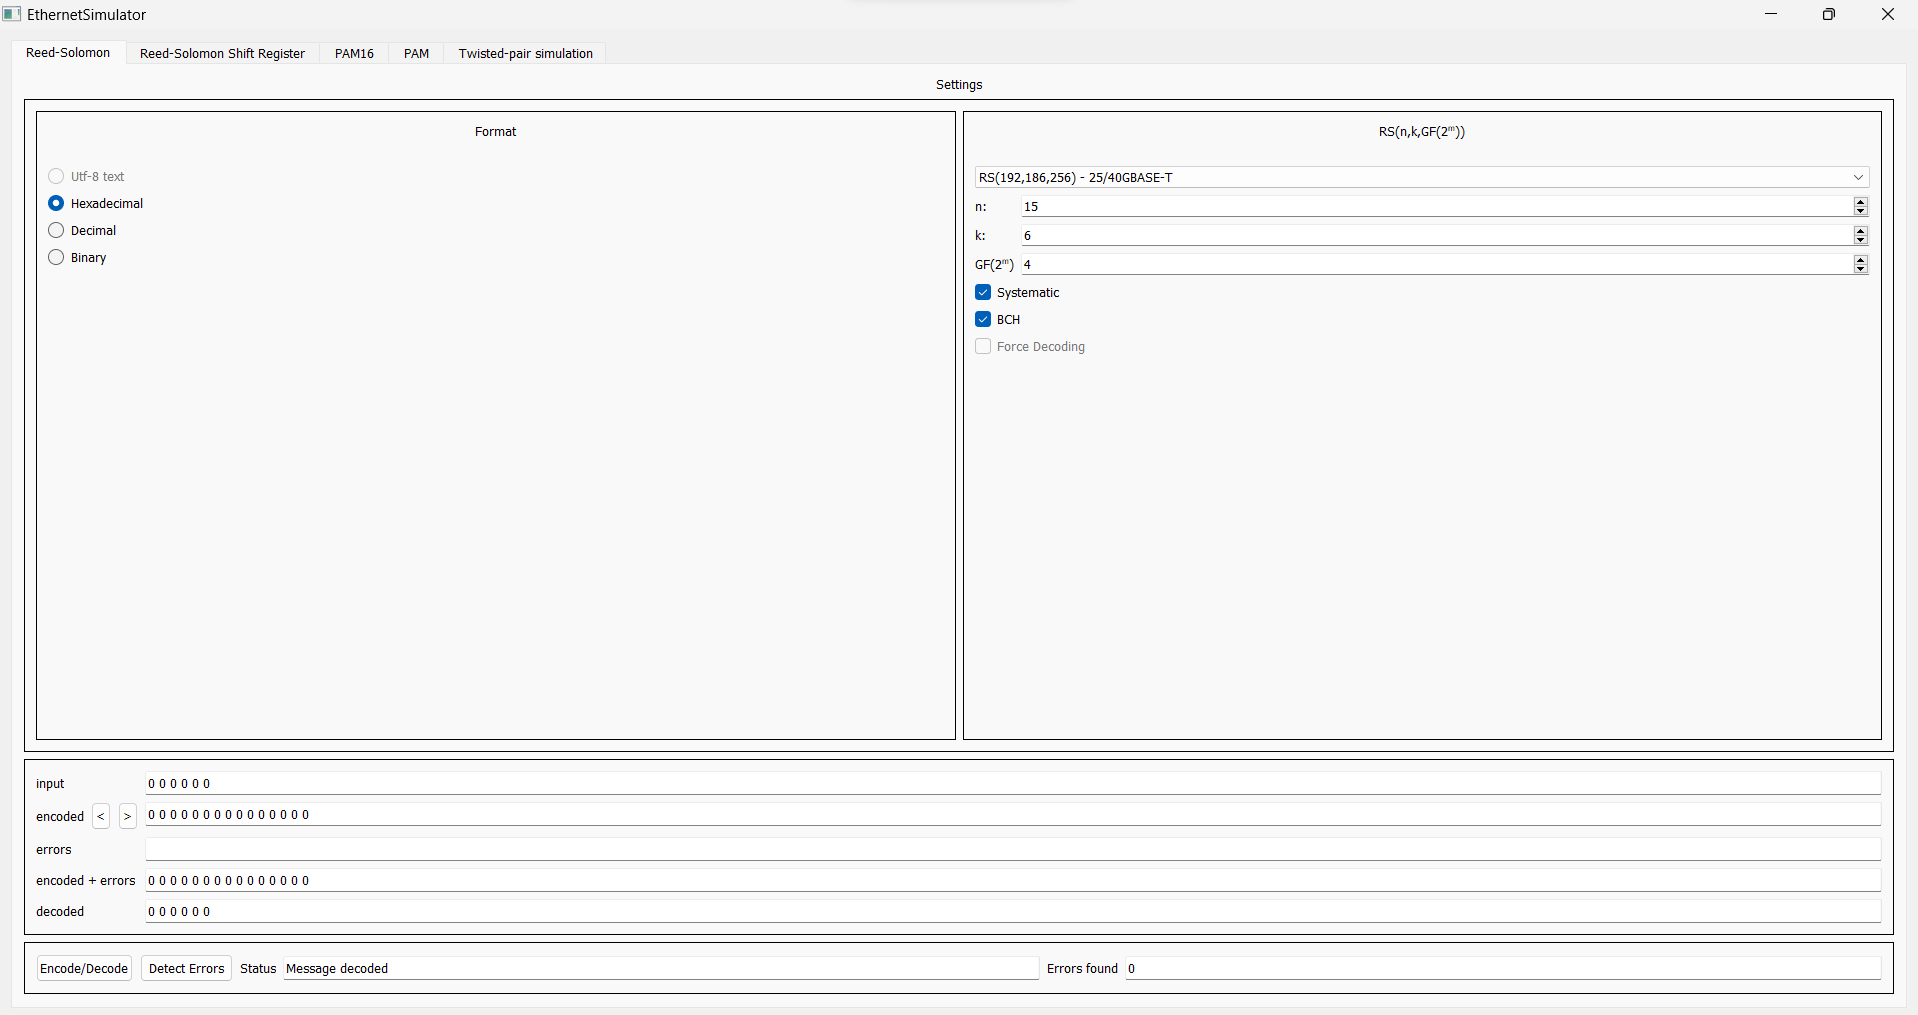
\includegraphics[width=\textwidth]{images/rozwiazania_1.png}
        \caption{Widok narzędzia Reed-Solomon podczas wykonywania zadania 1.}
        \label{fig:rozwiazania_1}
    \end{figure}
    
    \item Zakładka: Reed-Solomon, ustawienia programu: $n = 7$, $k = 3$, $GF = 2^3$,
    kod systematyczny BCH, tryb dziesiętny, wiadomość wejściowa `1 2 3'.
    Sprawdź dla błędów `3', `3 2', `3 2 1' oraz `3 2 1 4' czy dekoder jest w stanie
    wykryć błędy oraz czy jest w stanie je poprawić a jeżeli tak to czy poprawnie.
    Czy wiesz dlaczego pojawiły się rozbieżności między błędami poprawionymi a wykrytymi? \\ \\
    Odpowiedź: Według właściwości kodu Reeda-Solomona opisanych w sekcji~\ref{subsection:wlasciwosci} jest on w stanie poprawić $\lfloor \frac{n-k}{2} \rfloor$ błędnych symboli i wykryć $n-k$ błędnych symboli.
    W tym zadaniu wszystkie błędy były wykryte i jedynie $\lfloor \frac{n-k}{2} \rfloor$ czyli 2 błędy były poprawnie skorygowane.
    Odpowiedź 2: Ponieważ kod Reeda-Solomona jest w stanie wykryć 2 razy więcej
    błędów niż poprawić.
    \begin{table}[H]
        \renewcommand{\arraystretch}{1.8}
        \centering
        \begin{tabular}{|c|c|c|>{\centering\arraybackslash}p{5cm}|}
            \hline
            \textbf{Błąd} & \textbf{Wykrywa [TAK/NIE]} & \textbf{Poprawia [Ile]} & \textbf{Poprawia poprawnie [TAK/NIE]} \\
            \hline
            3 & TAK & 1 & TAK \\
            \hline
            3 2 & TAK & 2 & TAK \\
            \hline
            3 2 1 & TAK & 2 & NIE \\
            \hline
            3 2 1 4 & TAK & 2 & NIE \\
            \hline
        \end{tabular}
    \end{table}

    \begin{figure}[H]
        \centering
        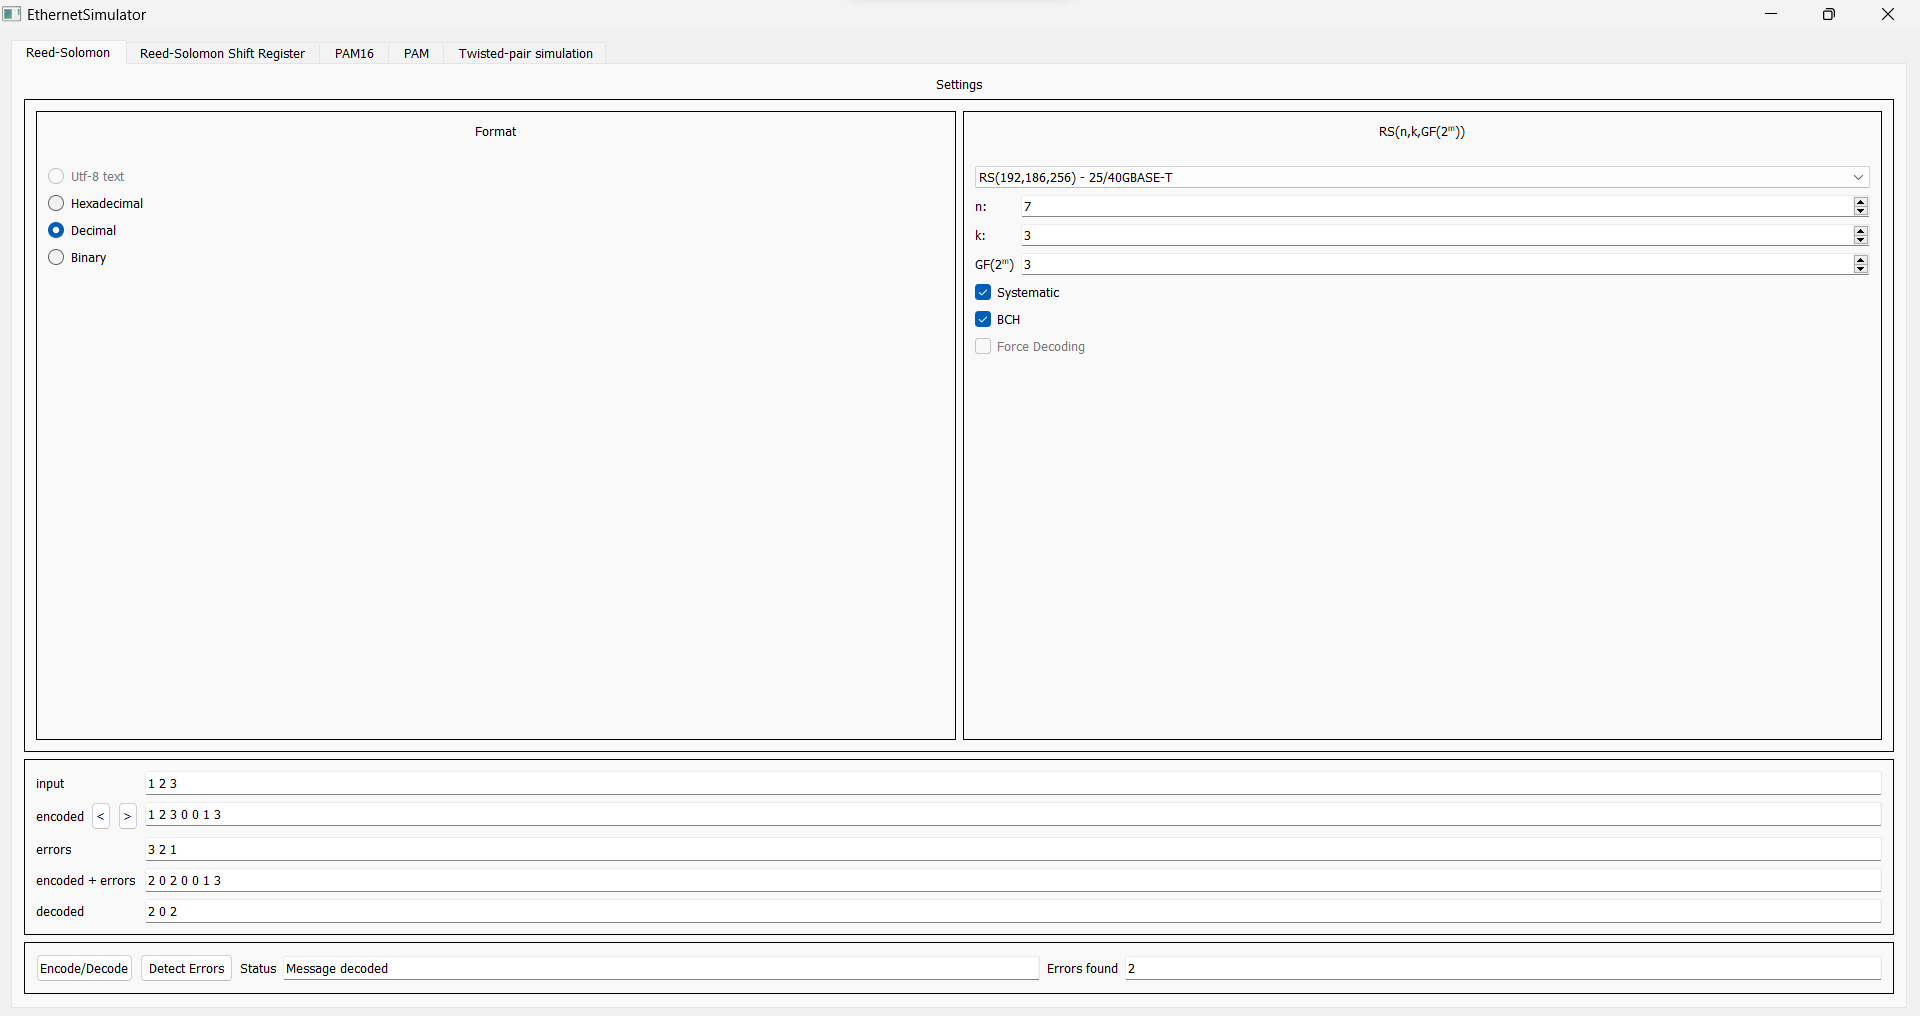
\includegraphics[width=\textwidth]{images/rozwiazania_2.png}
        \caption{Widok narzędzia Reed-Solomon podczas wykonywania zadania 2.}
        \label{fig:rozwiazania_2}
    \end{figure}
    
    \item Zakładka: Reed-Solomon Shift Register, ustawienia programu:
    $n = 3$, $k = 2$, $GF = 2^2$. Oblicz wielomian prymitywny i generator naciskając
    przycisk `Calculate primitive poly/element'.
    Zakoduj wiadomość: `2 1' w symulatorze po czym zakoduj wiadomość
    używając wzoru z sekcji `Systematyczny kod BCH'. Porównaj wyniki.
    \\ \\
    Odpowiedź: Zakodowana wiadomość to: `2 1 3'. Dla $p_m(x) = 2x + 1$ oraz $g(x) = x + 1$ słowo kodowe
    obliczone wzorem i przez symulator są takie same.
    \begin{equation*}
        \begin{aligned}[t]
            s_r(x) &= (2x+1) \cdot x \mod x + 1 \\
            s_r(x) &= 2x^2 + x \mod x + 1 \\
            s_r(x) &= 3 \\
            s(x) &= (2x+1) \cdot x - s_r(x) \\
            s(x) &= 2x^2 + x + 3 \\
            s(x) &= (2,1,3)
        \end{aligned}
    \end{equation*}

    

    \begin{figure}[H]
        \centering
        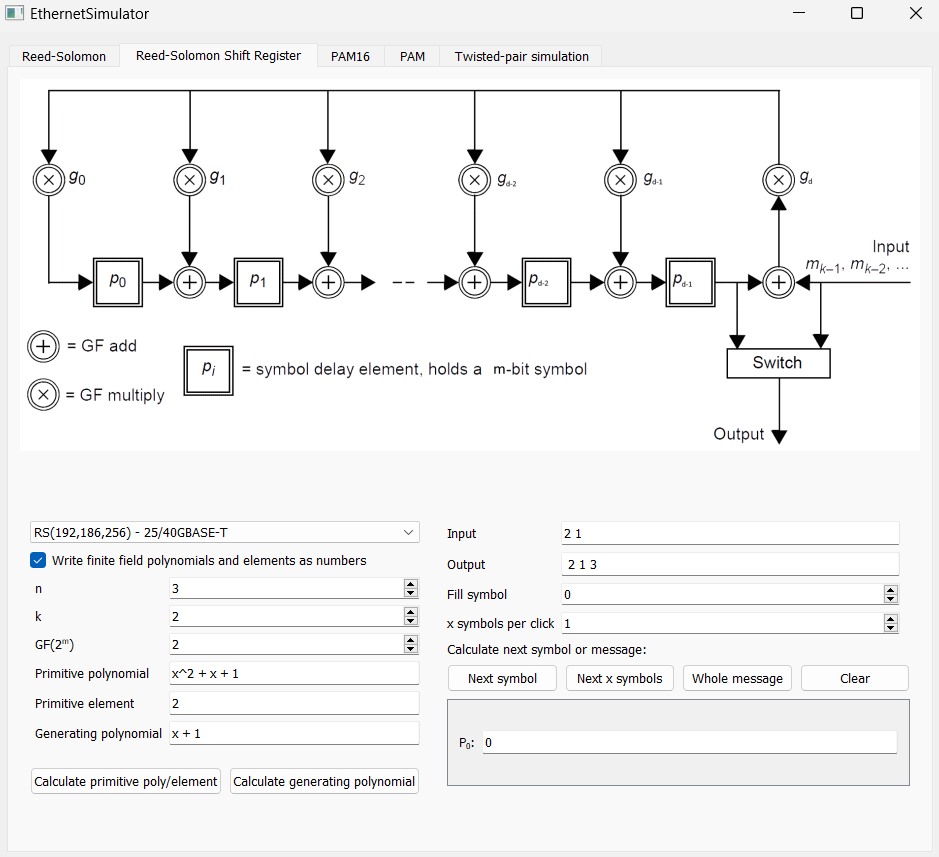
\includegraphics[width=\textwidth]{images/rozwiazania_3.png}
        \caption{Widok narzędzia Reed-Solomon Shift Register podczas wykonywania zadania 3.}
        \label{fig:rozwiazania_3}
    \end{figure}
    
    \item Zakładka: Reed-Solomon, ustawienia programu: $n = 15$, $k=7$, $GF = 2^4$,
    kod systematyczny BCH.
    Zakoduj dowolną niezerową $k$-symbolową wiadomość. Sprawdź czy przesunięcia słowa kodowego
    (z użyciem strzałek przy słowie `encoded') także będą słowem kodowym. \\ \\
    Odpowiedź: Dla wiadomości `1 2 3 4 5 6 7' wszystkie przesunięcia były poprawnie i bezbłędnie dekodowane.
    

    \begin{figure}[H]
        \centering
        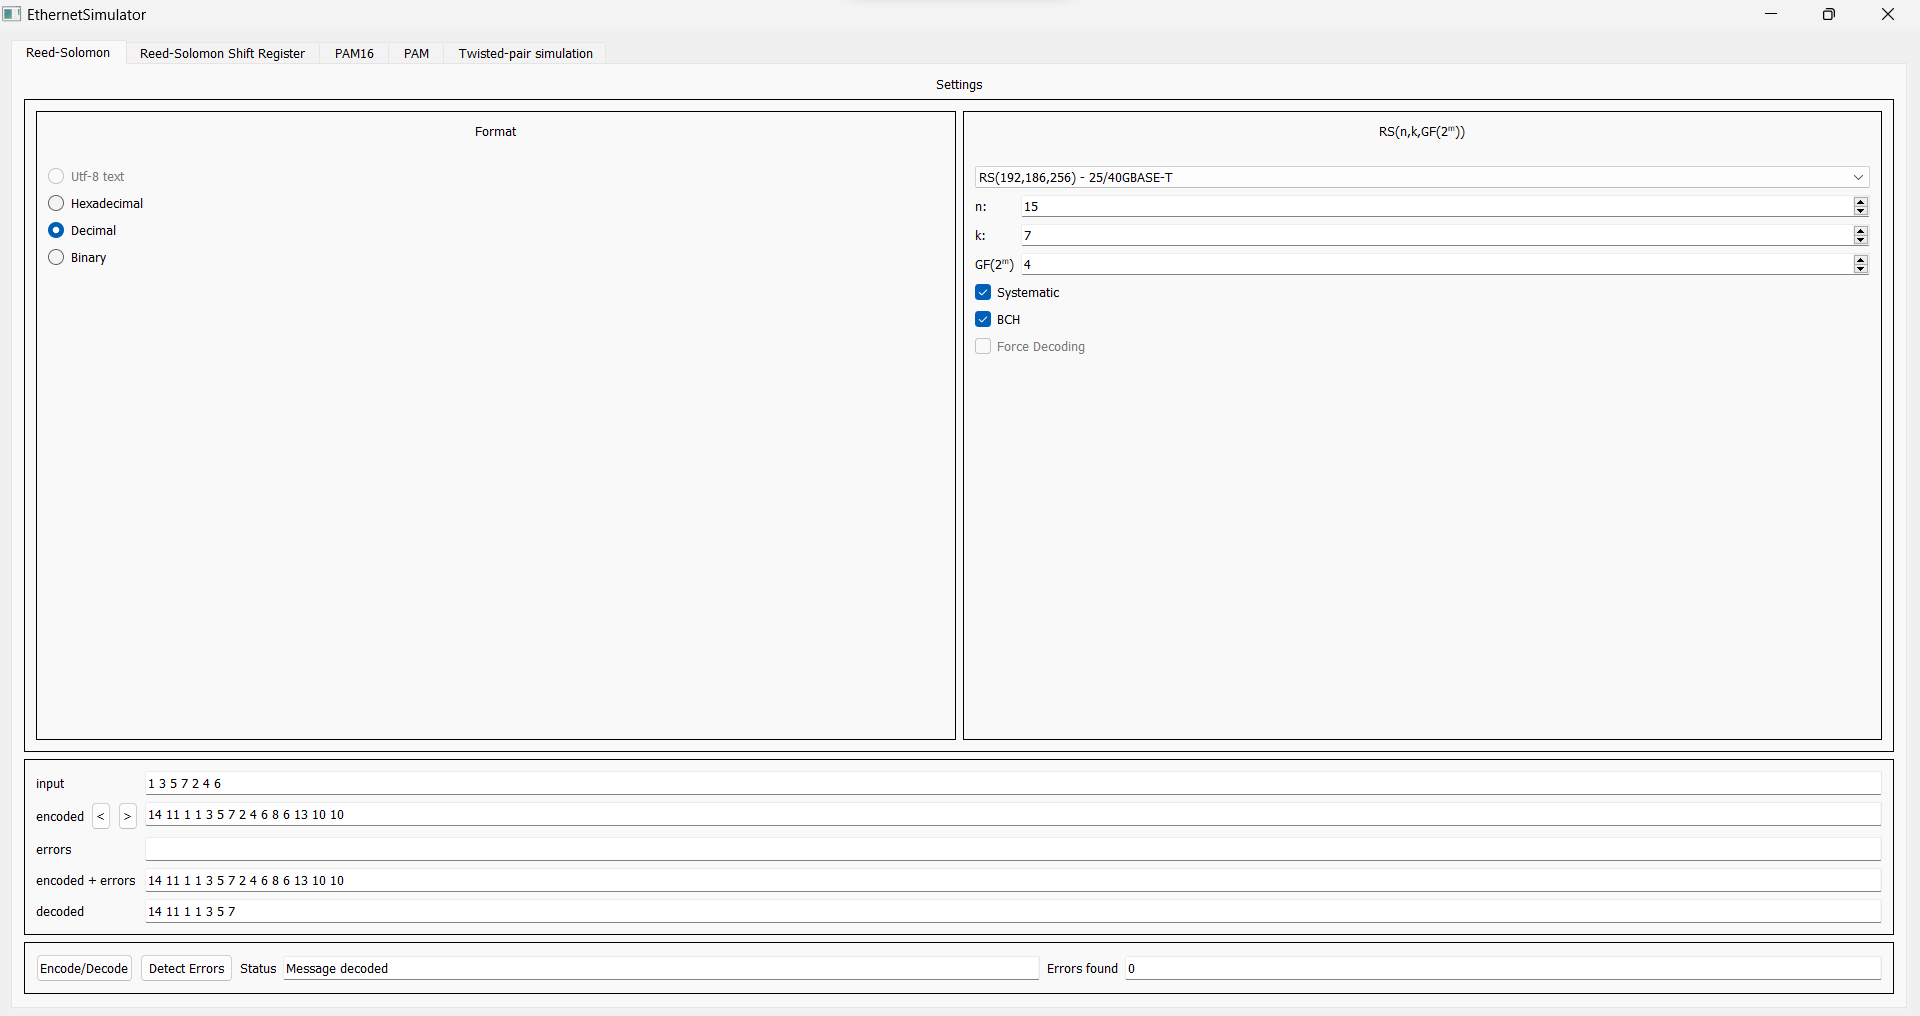
\includegraphics[width=\textwidth]{images/rozwiazania_4.png}
        \caption{Widok narzędzia Reed-Solomon podczas wykonywania zadania 4.}
        \label{fig:rozwiazania_4}
    \end{figure}
    
    \item Zakładka: PAM, Zamień numer swojego indeksu na postać szesnastkową i wykorzystaj go jako liczbę do przesłania. Przeprowadź symulację. Zanotuj w sprawozdaniu
    przybliżony czas transmisji oraz liczbę poziomów natężenia. Opisz wnioski, które nasuwają Ci się po wykonanym ćwiczeniu. \\ \\
    Odpowiedź:
    \begin{itemize}
        \item NRZ: 62ns, dwa poziomy
        \item PAM4: 33ns, cztery poziomy
        \item PAM16: 17ns, cztery poziomy (przesyłany numer indeksu jest na tyle mały, że nie wszystkie poziomy zostaną wykorzystane)
    \end{itemize}
    Stosowanie modulacji PAM wyższych poziomów pozwala na lepsze upakowanie danych, ale różnica pomiędzy wysyłanymi symbolami maleje.
    

    \begin{figure}[H]
        \centering
        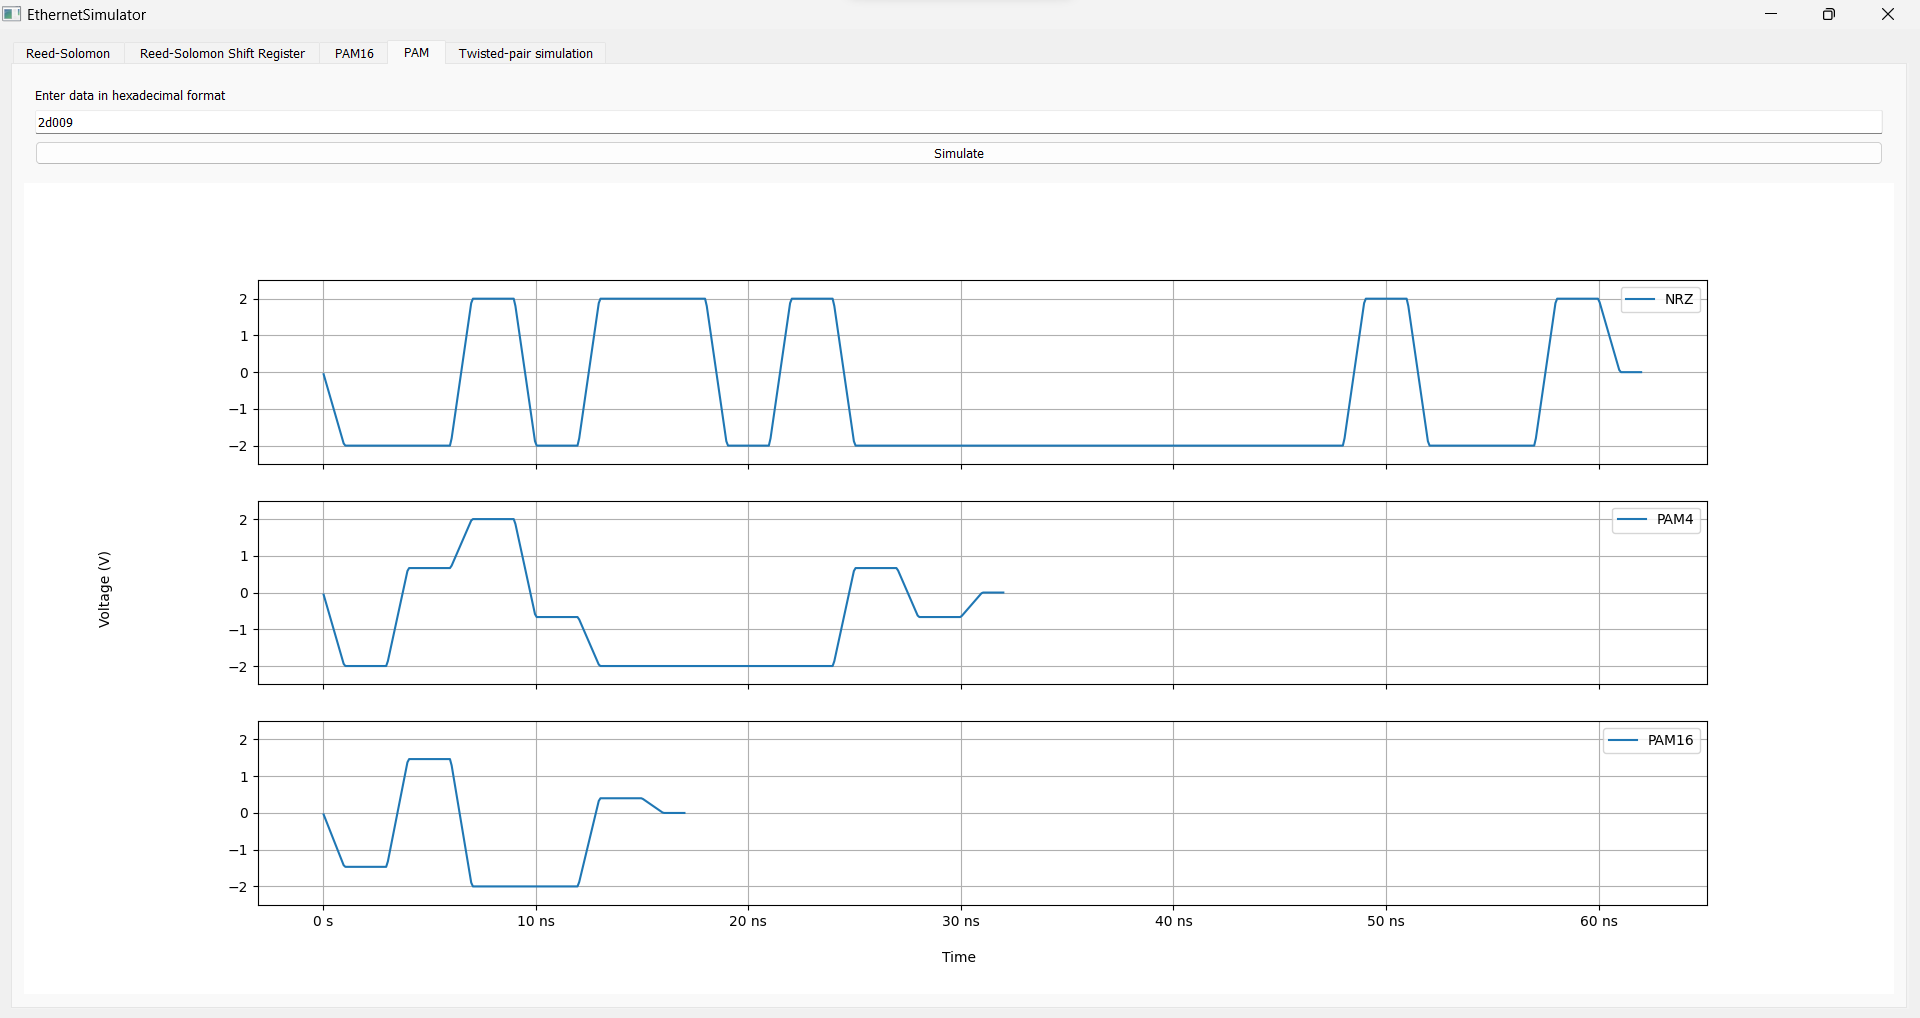
\includegraphics[width=\textwidth]{images/rozwiazania_5.png}
        \caption{Widok narzędzia PAM podczas wykonywania zadania 5.}
        \label{fig:rozwiazania_5}
    \end{figure}
    
    \item Zakładka: PAM, Prześlij ciąg składający się z samych jedynek (fffffff \dots) lub zer (000000 \dots). Popatrz na wynik symulacji. Jak nazywa się zaobserwowane zjawisko? Czy znasz sposoby,
    które zapobiegają jego wystąpieniu? Zanotuj w sprawozdaniu. \\ \\
    Odpowiedź: Na symulacji widać stałą składową. Można jej zapobiegać używając np. kodowania liniowego 64b/66b albo skramblera.
    
    

    \begin{figure}[H]
        \centering
        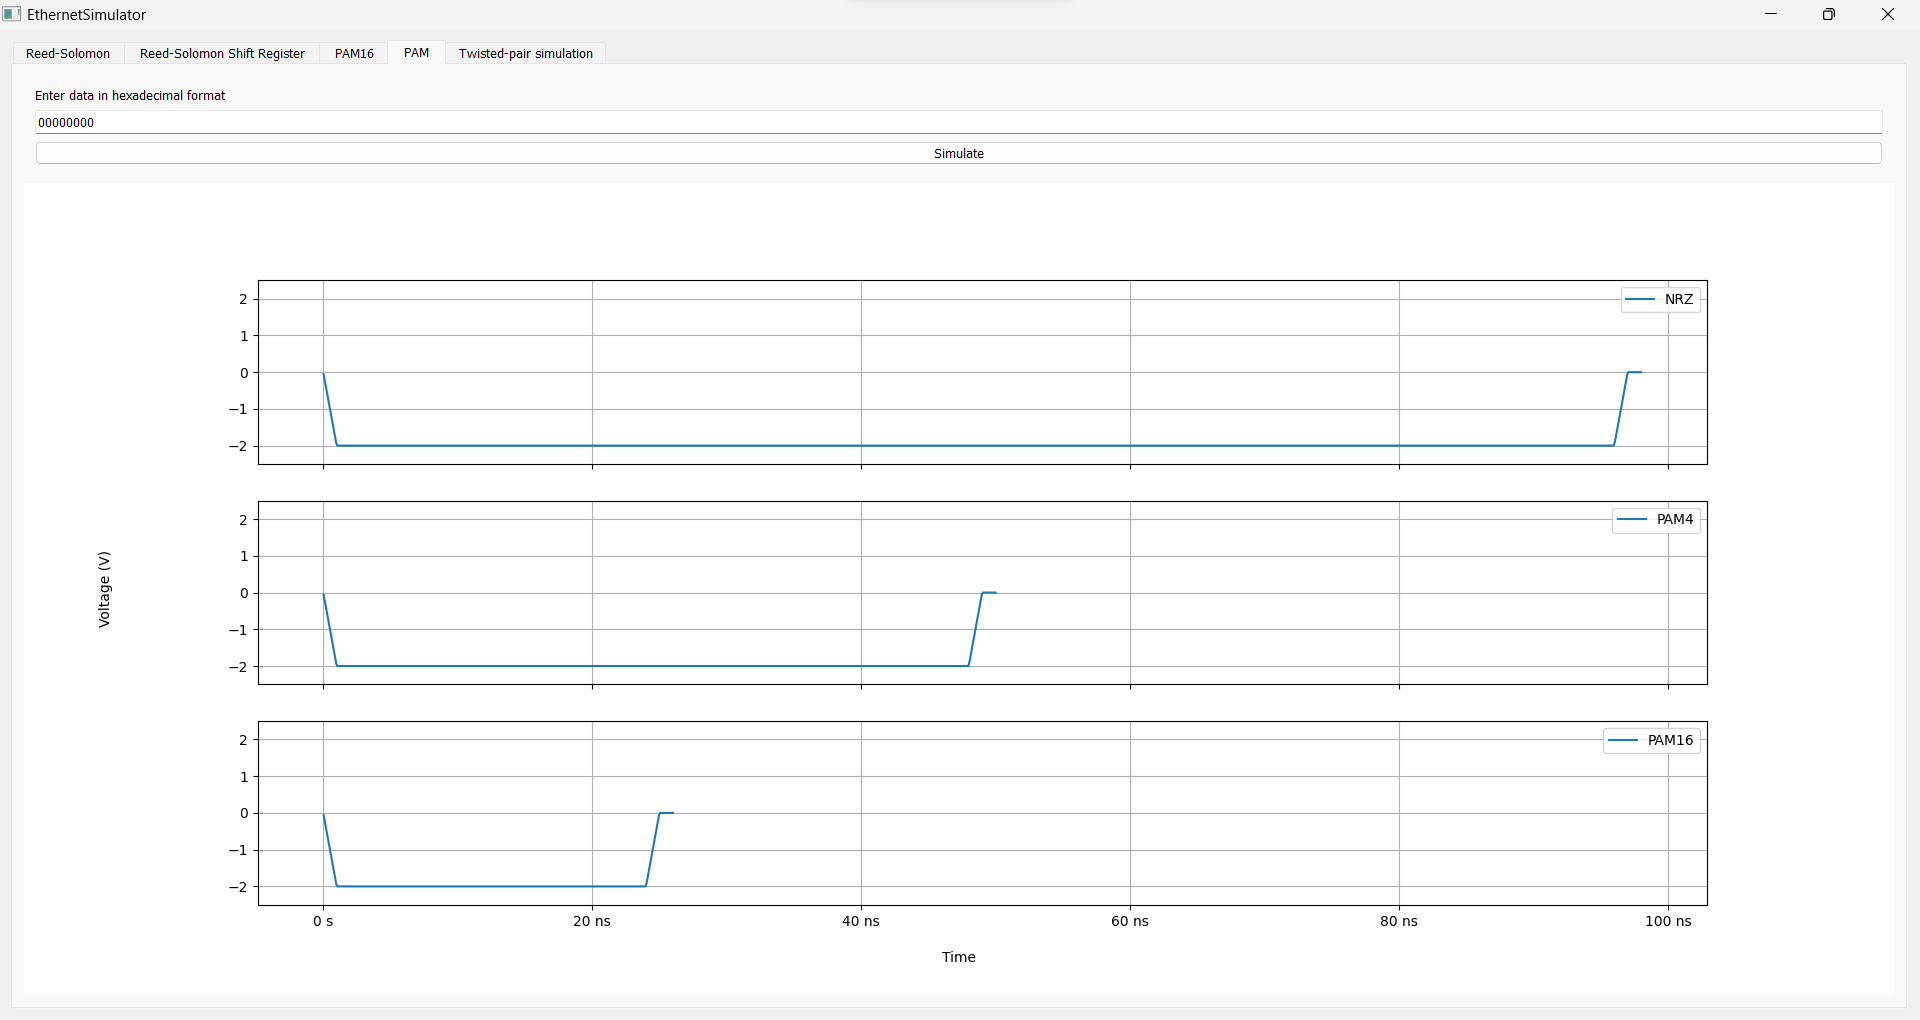
\includegraphics[width=\textwidth]{images/rozwiazania_6.png}
        \caption{Widok narzędzia PAM podczas wykonywania zadania 6.}
        \label{fig:rozwiazania_6}
    \end{figure}
    
    \item Zakładka: PAM16, Zastosowanie DSQ128 nie eliminuje możliwości wystąpienia stałej składowej. Znajdź ciąg, który
    temu dowodzi i zanotuj go w sprawozdaniu. \\ \\
    Odpowiedź: Na przykład: 0x000000 \dots, 0x111111 \dots (0b000100010001 \dots),\\0x22222 \dots (0b001000100010 \dots),
    0x444444 \dots (0b010001000100 \dots).

    

    \begin{figure}[H]
        \centering
        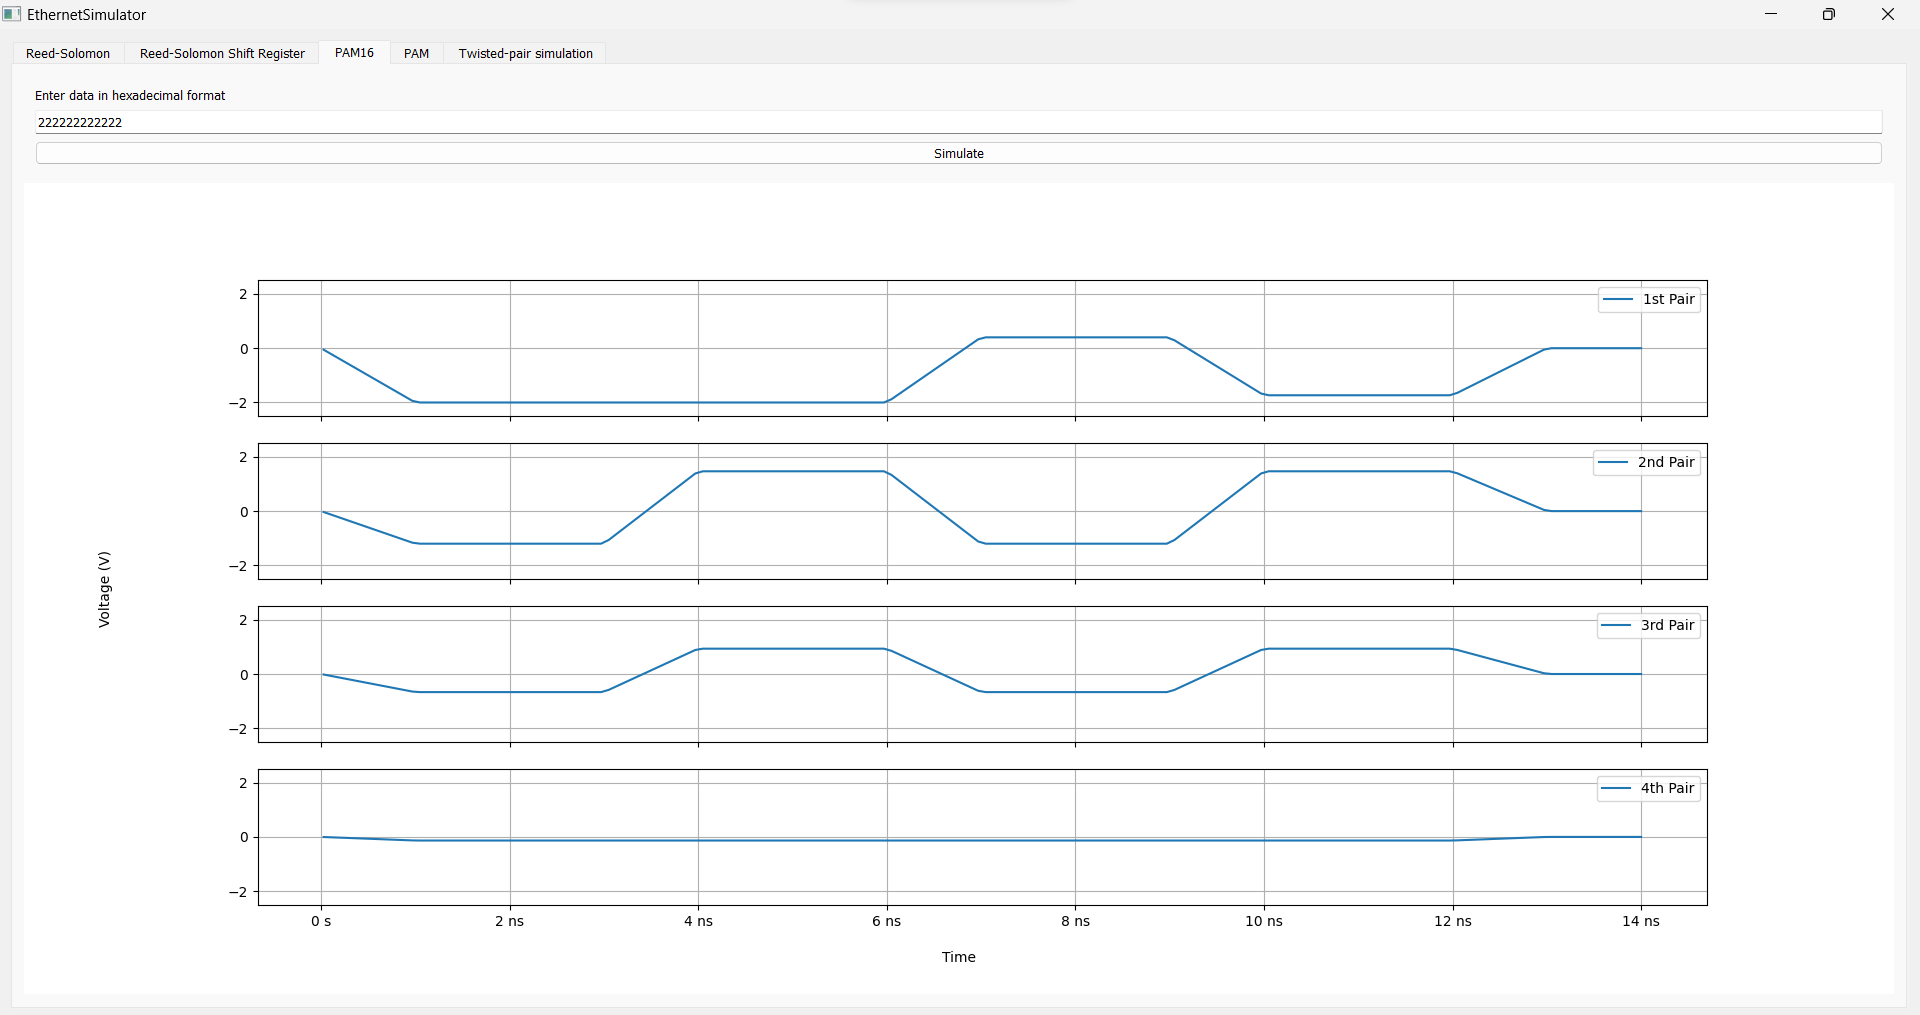
\includegraphics[width=\textwidth]{images/rozwiazania_7.png}
        \caption{Widok narzędzia PAM podczas wykonywania zadania 7.}
        \label{fig:rozwiazania_7}
    \end{figure}
    
    \end{enumerate}

\subsection*{Wnioski}

W naszej ocenie przygotowane w ramach niniejszej pracy zadania laboratoryjne powinny w dobry sposób przybliżyć studentom podstawy
teoretyczne oraz aspekty praktyczne poruszanych w nich zagadnień. Zadania są krótkie i stosunkowo łatwe do rozwiązania, dzięki czemu
student nie jest poddany presji czasu. Zaprojektowany symulator wizualizuje omawiane rozwiązania warstwy fizycznej Ethernet, co byłoby
trudne i wymagałoby wysokiej jakości sprzętu, jeżeli realizacja przebiegałaby na rzeczywistym sprzęcie.


\setcounter{secnumdepth}{0}
\section*{Dodatek G: Symulacja tłumienia}
\addcontentsline{toc}{section}{\protect\numberline{}Dodatek G: Symulacja tłumienia}

\subsection{Wstęp}
Symulacja przejścia sygnału przez kanał została zrealizowana za pomocą symulatora
SPICE jednak użyty model linii transmisyjnej nie symulował tłumienia.
Próba zaimplementowania własnego modelu skończyła się niepowodzeniem z powodu
dużych częstotliwości co powodowało bardzo długie działanie programu ngspice i
ewentualne nagłe zakończenie działania programu z powodu błędów.

\subsection{Obliczanie tłumienia}
Tłumienie zostało obliczone za pomocą wzoru~(\ref{tlumienie})~\cite[sekcja 4.3.4.7]{TIA/EIA-568-B}
\begin{align}
    k_1 \cdot \sqrt{f} + k_2 \cdot f + \frac{k_3}{\sqrt{f}}\label{tlumienie}
\end{align}
gdzie $f$ to częstotliwość, $k_1$ to straty spowodowane efektem naskórkowości,
$k_2$ to straty spowodowane materiałem przewodnika a $k_3$ to straty spowodowane
przez użycie ekranowania

Wartości $k_1$, $k_2$, $k_3$ dla różnych kabli podane są w tabeli~\ref{tab:tlumienie}
\begin{table}
    \captionof{table}{Stałe tłumienia}
    \centering
    \begin{tabular}{c c c c}
        \toprule
        \textbf{Kabel} & \textbf{$k_1$} & \textbf{$k_2$} & \textbf{$k_3$} \\
        \toprule
        Cat5~\cite{IEEE-cabling} & 1.9108 & 0.0222 & 0.2 \\
        \midrule
        Cat5e~\cite[sekcja 4.3.4.7]{TIA/EIA-568-B} & 1.967 & 0.023 & 0.05 \\
        \midrule
        Cat6~\cite{IEEE-cabling} & 1.82 & 0.0169 & 0.25 \\
        \midrule
        Cat7~\cite{IEEE-cabling} & 1.8 & 0.01 & 0.2
    \end{tabular}\label{tab:tlumienie}
\end{table}


\end{document}
